\documentclass[conference]{IEEEtran}
\IEEEoverridecommandlockouts

\usepackage{fontspec}
\usepackage{polyglossia}
\setmainlanguage{portuges}
\usepackage{amsmath,amssymb,amsfonts}
\usepackage{graphicx}
\usepackage{textcomp}
\usepackage{xcolor}
\usepackage{booktabs}
\usepackage{array}
\usepackage{multirow}
\usepackage{url}
\usepackage[hidelinks]{hyperref}

\def\BibTeX{{\rm B\kern-.05em{\sc i\kern-.025em b}\kern-.08em
    T\kern-.1667em\lower.7ex\hbox{E}\kern-.125emX}}

\begin{document}

\title{Modelagem Algorítmica em Árvores Genealógicas de 5 Gerações (DAG) e Teoria dos Grafos Aplicada ao Turfe Japonês de Elite (2002--2025): Bijeção Topológica BFS/DFS, PageRank Esportivo, Endogamia de Wright e Aprendizado de Máquina\\
{\footnotesize \textnormal{Trabalho Final: Estruturas em Árvores e Teoria dos Grafos (AEDS II) --- Centro Federal de Educação Tecnológica de Minas Gerais (CEFET-MG)}}
}

\author{
\IEEEauthorblockN{1\textsuperscript{º} Arthur De Oliveira Mendonça}
\IEEEauthorblockA{\textit{Departamento de Computação e Mecatrônica} \\
\textit{Centro Federal de Educação Tecnológica de Minas Gerais (CEFET-MG)}\\
Divinópolis, Minas Gerais, Brasil \\
Repositório: \url{https://github.com/ImArthz/AEDS2_jra_analysis}}
\and
\IEEEauthorblockN{2\textsuperscript{º} Michel Pires da Silva}
\IEEEauthorblockA{\textit{Departamento de Computação e Mecatrônica} \\
\textit{Centro Federal de Educação Tecnológica de Minas Gerais (CEFET-MG)}\\
Divinópolis, Minas Gerais, Brasil \\
Dataset Zenodo DOI: \url{https://doi.org/10.5281/zenodo.23681383}}
}

\maketitle

\begin{abstract}
A análise histórica da \textit{Japan Racing Association} (JRA, 2002--2025, 3.216 corridas e 33.409 participações) e das árvores genealógicas de 5 gerações do \textit{Japan Bloodhorse Information System} (JBIS, 504.074 nós) enfrenta anomalias estruturais severas (inversão topológica entre Busca em Profundidade e Busca em Largura e fusão de colunas em 25.014 registros), barreiras semânticas do japonês e a miopia da contagem simples de vitórias. Para solucioná-las, desenvolveu-se um pipeline em Python (Linux Ubuntu 24.04) integrando realinhamento vetorial, bijeção topológica $\text{DFS}\to\text{BFS}$, tradução híbrida por IA (29.159 termos), algoritmos em árvores e grafos (PageRank, BFS, DFS, Menor Ancestral Comum --- LCA, Endogamia de Wright $F_X$ e Dijkstra) e aprendizado de máquina sem vazamento temporal. O domínio foi modelado em listas de adjacência esparsas: (i) Árvores Binárias de 5 gerações (62 ancestrais/animal) contraídas em um Grafo Direcionado Acíclico (DAG) $G_p$ ($|V_p|=35.149, |E_p|=63.007$); (ii) um Grafo Direcionado Ponderado de Competição $G_c$ ($|V_c|=8.135, |E_c|=195.271$); e (iii) dois Grafos Bipartidos ($G_{jc}, G_{jt}$). Operando em tempo linear $O(V+E)$, o PageRank ($d=0,85, r=0,8799$ com pódios) descobriu ``Diamantes Injustiçados'' com zero vitórias Graded (\textit{Sounds of Earth}, \#32 entre 8.135 cavalos); o algoritmo de Wright identificou \textit{Northern Dancer} como maior patriarca LCA (4.206 cavalos endogâmicos e 1.211 vitórias); o K-Means++ via PCA 2D (63,4\% de variância) isolou 4 arquétipos paternos ($\chi^2=2237,47, p<10^{-300}$); e a \textit{Random Forest Out-of-Time} atingiu $\text{ROC-AUC}=0,7260$, integrando redes Gephi, dashboard \textit{Apache Superset/ECharts} e uma arena gamificada de 520 cards (TCG).
\end{abstract}

\begin{IEEEkeywords}
Estruturas em Árvores, Teoria dos Grafos, Grafo Direcionado Acíclico (DAG), Bijeção Topológica BFS/DFS, PageRank Esportivo, Coeficiente de Endogamia de Wright, Algoritmo de Dijkstra, Aprendizado de Máquina, Visualização de Redes Complexas.
\end{IEEEkeywords}

\section{Introdução}
As estruturas de dados não-lineares --- em especial as árvores hierárquicas, os Grafos Direcionados Acíclicos (\textit{Directed Acyclic Graphs} --- DAGs) e as redes complexas ponderadas --- constituem o alicerce matemático e computacional da ciência da computação moderna, viabilizando desde o roteamento em redes de telecomunicações e sistemas de navegação até a análise de topologias sociais, triagem molecular e genômica populacional [1, 2, 9]. Na biologia computacional e na zootecnia de precisão, a representação da ancestralidade biológica por meio de árvores binárias ascendentes e sua subsequente contração topológica em DAGs permitem quantificar a consanguinidade, rastrear a transmissão de alelos de alta performance e identificar gargalos genéticos ao longo de múltiplas gerações [3, 4]. Paralelamente, na ciência dos esportes de alto rendimento, a modelagem de confrontos diretos como grafos direcionados de fluxo de prestígio supera as limitações de métricas tabulares estáticas, capturando a força relativa dos oponentes através de processos estocásticos sobre cadeias de Markov [5, 7].

Afunilando esse panorama teórico para um problema real de alta relevância econômica e biológica, destaca-se a indústria do turfe japonês de elite, administrada pela \textit{Japan Racing Association} (JRA) em conjunto com o repositório genealógico do \textit{Japan Bloodhorse Information System} (JBIS) [14]. Movimentando bilhões de dólares anualmente em premiações e leilões de reprodutores Puro-Sangue Inglês (\textit{Thoroughbred}), o circuito japonês funciona como um laboratório empírico rigorosamente controlado: cada corrida graduada (\textit{Graded Race} de Grau 1, Grau 2 ou Grau 3) documenta variáveis físicas, cinemáticas, ambientais e humanas com precisão de décimos de segundo, enquanto cada competidor possui sua árvore genealógica completa de 5 gerações ascendentes ($2^1 + 2^2 + 2^3 + 2^4 + 2^5 = 62$ ancestrais) catalogada. No mundo real, decisões de cruzamento genético (\textit{nicking} e \textit{linebreeding}) e a avaliação do valor reprodutivo de garanhões dependem diretamente da análise conjunta dessa árvore genealógica de 5 gerações e da rede histórica de confrontos em pista.

Entretanto, a transformação de 24 anos de registros brutos da JRA e do JBIS (2002--2025) em estruturas em árvores e grafos computacionalmente íntegras esbarra em quatro obstáculos técnicos severos que motivaram a escolha deste tema:
\begin{enumerate}
    \item \textbf{Inversão Topológica entre Busca em Profundidade (DFS) e Busca em Largura (BFS) em Árvores HTML:} O portal JBIS renderiza a árvore genealógica de 5 gerações utilizando tabelas HTML aninhadas com atributo \texttt{rowspan} progressivo ($16, 8, 4, 2, 1$). No fluxo de marcação DOM, as células aparecem ordenadas geração por geração (ordem de Busca em Largura --- BFS), ao passo que algoritmos de raspagem sequenciais rotulam os caminhos genealógicos (\texttt{S}, \texttt{SS}, \texttt{SSS}...) em pré-ordem de Busca em Profundidade (DFS). Sem uma bijeção matemática formal de realinhamento, as arestas pai-filho de 504.074 nós ancestrais tornam-se topologicamente corrompidas.
    \item \textbf{Mutação Histórica de Esquemas e Deslocamento Vetorial (2002--2025):} Entre 2006 e 2018, os registros da JRA fundiram as colunas de Sexo e Idade em um único campo composto (coluna \textit{Seirei}, ex.: \texttt{Male-4}), provocando um deslocamento vetorial à esquerda em 25.014 participações que desalinhou vértices de jóqueis, treinadores, tempos e massas corporais.
    \item \textbf{Ambiguidade Semântica e Homonímia em Grafos Bilíngues:} Nomes equinos em \textit{Katakana} (estrangeirismos fonéticos em inglês, francês e italiano), antropônimos humanos em \textit{Kanji} com leitura especial \textit{Nanori} e 15 campeões históricos homônimos entre a base japonesa e registros internacionais geram colapsos indevidos de vértices ou perda de conectividade quando submetidos a transliteradores fonéticos convencionais.
    \item \textbf{Miopia da Contagem Simples de Vitórias e Vazamento Temporal (\textit{Data Leakage}):} Métricas escalares tradicionais classificam cavalos apenas pelo número bruto de vitórias, descartando animais que competiram exclusivamente na elite de Grau 1 e acumularam múltiplos vice-campeonatos contra lendas históricas. Além disso, modelos preditivos que utilizam estatísticas agregadas de fim de carreira incorrem em vazamento temporal do futuro para o passado.
\end{enumerate}

Diante desse cenário, o \textbf{objetivo geral} desta pesquisa é projetar, implementar e validar um arcabouço algorítmico completo em estruturas em árvores e teoria dos grafos, integralmente compatível com execução via terminal em Linux (Ubuntu 24.04) e publicado com dados abertos sob identificador DOI no Zenodo [14], capaz de modelar 24 temporadas da JRA (3.216 corridas e 33.409 participações) e 5 gerações do JBIS (504.074 nós genealógicos). De forma específica, objetiva-se: (i) formalizar e executar a bijeção topológica $1\text{-para-}1$ de $\text{DFS}\to\text{BFS}$ sobre as 8.202 árvores binárias de 5 gerações e contraí-las em um DAG Genealógico unificado $G_p = (V_p, E_p)$ com $|V_p| = 35.149$ ancestrais únicos e $|E_p| = 63.007$ arestas direcionadas; (ii) implementar algoritmos lineares $O(V + E)$ de travessia BFS/DFS, detecção de Menor Ancestral Comum (LCA) e cálculo exato do Coeficiente de Endogamia de Wright ($F_X$) [3, 4]; (iii) construir o Grafo Direcionado Ponderado de Competição $G_c = (V_c, E_c, W)$ ($|V_c| = 8.135, |E_c| = 195.271$) e aplicar os algoritmos de PageRank Esportivo ($d = 0,85$) [5, 7], Componentes Conexos via BFS e Caminho Mínimo de Dijkstra [8] para descobrir talentos de elite ocultos (``Diamantes Injustiçados''); (iv) acoplar as métricas topológicas dos grafos a testes estatísticos ($\chi^2$, ANOVA, Kruskal-Wallis), clusterização K-Means++ via PCA 2D [12] e classificação supervisionada \textit{Random Forest Out-of-Time} sem vazamento temporal [13]; e (v) disponibilizar representações visuais vetoriais no software Gephi (\textit{ForceAtlas2}) [10, 11], uma suíte executiva interativa baseada no motor \textit{Apache ECharts 5.5 / Apache Superset 6.1} e uma arena gamificada de 520 cards colecionáveis (TCG).

O restante deste artigo está organizado da seguinte forma: a \textbf{Seção II} apresenta o Referencial Teórico e o Estado da Arte das estruturas em árvores binárias, DAGs genealógicos, algoritmo de Wright, centralidade PageRank, algoritmo de Dijkstra e layouts baseados em força. A \textbf{Seção III} detalha a Metodologia, incluindo a natureza dos dados, a engenharia de limpeza e tradução híbrida por IA, a tradução formal do domínio em nós de árvores e vértices/arestas de grafos, a análise de complexidade assintótica e o fluxograma completo do ciclo de vida da solução. A \textbf{Seção IV} expõe os Resultados e Discussão, abrangendo benchmarks empíricos de tempo de execução e escalabilidade $O(V + E)$ entre 2002 e 2025, a descoberta dos ``Diamantes Injustiçados'' via PageRank, a estrutura endogâmica em 5 gerações, a modelagem preditiva e as aplicações web interativas (\textit{Superset Dashboard} e \textit{JRA TCG Card Arena}). Por fim, a \textbf{Seção V} sintetiza as Conclusões, as limitações enfrentadas, as instruções de reprodutibilidade em Linux e as direções para trabalhos futuros.

\section{Referencial Teórico (Estado da Arte)}
Esta seção fundamenta formalmente as estruturas de dados em árvores e grafos, bem como os algoritmos clássicos e contemporâneos adotados na modelagem do problema.

\subsection{Árvores Binárias de Ancestralidade, Travessias DFS/BFS e Contração em DAGs}
Em genealogia matemática, a árvore ascendente de um indivíduo $h_0$ até uma profundidade máxima de $g$ gerações é definida formalmente como uma \textbf{Árvore Binária Completa Enraizada} $T(h_0) = (V_T, E_T)$ de altura $g$ [1]. A raiz no nível $0$ representa o indivíduo focal $h_0$; para cada nó interno $u$ no nível $l \in \{0, \dots, g-1\}$, existem exatamente dois filhos na árvore ascendente: o ascendente paterno (\textit{Sire}, rotulado pelo sufixo $\texttt{S}$) e o ascendente materno (\textit{Dam}, rotulado pelo sufixo $\texttt{D}$) no nível $l + 1$. O número total de ancestrais estritos (excluindo a raiz $h_0$) em uma árvore de $g = 5$ gerações é dado pela soma geométrica finita:
\begin{equation}
    |V_T \setminus \{h_0\}| = \sum_{l=1}^{g} 2^l = 2^{g+1} - 2 = 62 \text{ nós} \quad (g = 5)
\end{equation}

Cada posição estrutural dentro de $T(h_0)$ é univocamente identificada por uma palavra binária $\omega \in \{\texttt{S}, \texttt{D}\}^+$ de comprimento $1 \le |\omega| \le 5$, onde o prefixo $\omega_{1 \dots |\omega|-1}$ identifica o nó filho imediato e o último símbolo $\omega_{|\omega|} \in \{\texttt{S}, \texttt{D}\}$ indica a relação paterna ou materna. A literatura clássica de estruturas de dados [1, 2] estabelece duas estratégias canônicas de enumeração linear dos nós de $T(h_0)$:
\begin{itemize}
    \item \textbf{Busca em Profundidade (\textit{Depth-First Search} --- DFS em Pré-Ordem):} Visita recursivamente a subárvore paterna completa até a folha de 5ª geração antes de retroceder (\textit{backtracking}) para as ramificações maternas, produzindo a sequência lexicográfica de profundidade $(\texttt{S}, \texttt{SS}, \texttt{SSS}, \texttt{SSSS}, \texttt{SSSSS}, \texttt{SSSSD}, \dots, \texttt{DDDDD})$.
    \item \textbf{Busca em Largura (\textit{Breadth-First Search} --- BFS por Níveis):} Utiliza uma fila FIFO (\textit{First-In, First-Out}) para visitar todos os $2^l$ nós da geração $l$ antes de avançar para a geração $l+1$, ou, no caso de tabelas HTML com células mescladas por \texttt{rowspan} $= 2^{5-l}$, enumera os nós na ordem geométrica das linhas de renderização visual da tabela.
\end{itemize}

Embora cada indivíduo $h_0$ possua $62$ posições teóricas em sua árvore binária $T(h_0)$, em populações biológicas reais sob seleção artificial ocorre o fenômeno de \textbf{colapso de pedigree} (\textit{pedigree collapse} ou endocruzamento): um mesmo ancestral biológico $A$ aparece em múltiplos caminhos distintos $\omega_1 \neq \omega_2$ dentro da mesma árvore ou através das árvores de múltiplos indivíduos [3, 4]. Quando fundimos todas as árvores individuais $\{T(h_i)\}_{i=1}^{N}$ colapsando vértices de mesmo identificador biológico em um único nó e preservando a orientação temporal das arestas (do filho para o progenitor ou vice-versa), a floresta de árvores binárias contrai-se em um \textbf{Grafo Direcionado Acíclico (\textit{Directed Acyclic Graph} --- DAG)} $G_p = (V_p, E_p)$ [1, 4]. A aciclicidade de $G_p$ é garantida por um invariante biológico temporal estrito: nenhum organismo pode ser ancestral de si mesmo ($\text{ano\_nasc}(p) < \text{ano\_nasc}(u)$ para toda aresta $(u \to p) \in E_p$).

\subsection{Menor Ancestral Comum (LCA) em DAGs e Coeficiente de Endogamia de Wright ($F_X$)}
Sobre o DAG genealógico $G_p = (V_p, E_p)$, dois problemas algorítmicos fundamentais emergem na literatura: a determinação do \textbf{Menor Ancestral Comum (\textit{Lowest Common Ancestor} --- LCA)} [4] e o cálculo do \textbf{Coeficiente de Endogamia de Wright ($F_X$)} [3].

Dados dois vértices $u, v \in V_p$, denote-se por $\text{Anc}(u) = \{a \in V_p \mid d_{G_p}(u, a) \le g\}$ o conjunto de ancestrais alcançáveis a partir de $u$ em até $g$ passos direcionados, onde $d_{G_p}(u, a)$ é o comprimento do caminho mínimo calculado via Busca em Largura (BFS). Conforme formalizado por Bender et al. [4], o conjunto de ancestrais comuns é $C(u, v) = \text{Anc}(u) \cap \text{Anc}(v)$, e o Menor Ancestral Comum $\text{LCA}(u, v)$ é o vértice $a^* \in C(u, v)$ que minimiza a distância genealógica combinada:
\begin{equation}
    \text{LCA}(u, v) = \arg\min_{a \in C(u,v)} \left( d_{G_p}(u, a) + d_{G_p}(v, a) \right)
\end{equation}

Em 1922, Sewall Wright [3] formulou através do método de coeficientes de caminho (\textit{path analysis}) a probabilidade exata $F_X$ de que dois alelos homólogos em um indivíduo $X$ sejam idênticos por descendência (\textit{Identical by Descent} --- IBD). Seja $\mathcal{P}_{\min}(X)$ o conjunto de pares de caminhos minimais $(\omega_S, \omega_D)$ na árvore de 5 gerações de $X$ tais que $\omega_S$ pertence ao ramo paterno ($\omega_S[1] = \texttt{S}$), $\omega_D$ pertence ao ramo materno ($\omega_D[1] = \texttt{D}$), ambos convergem no mesmo ancestral comum $A$ na extremidade final e nenhum prefixo estrito de $(\omega_S, \omega_D)$ já intersecta o mesmo ramo (evitando dupla contagem dos pais do próprio ancestral comum $A$). Sendo $n_S = |\omega_S|$ e $n_D = |\omega_D|$ as distâncias em gerações de $X$ até $A$ pelos lados paterno e materno, o Coeficiente de Endogamia de Wright truncado em $g = 5$ gerações é dado por [3]:
\begin{equation}
    F_X = \sum_{(\omega_S, \omega_D, A) \in \mathcal{P}_{\min}(X)} \left(\frac{1}{2}\right)^{n_S + n_D - 1} (1 + F_A)
\end{equation}
Assumindo-se a linha de base de 5 gerações ($F_A = 0$ dentro da janela observada), um cruzamento clássico de $3 \times 4$ gerações ($n_S = 3, n_D = 4$) contribui exatamente com $(1/2)^{3+4-1} = (1/2)^6 = 0,015625$ ($1,5625\%$) por ancestral duplicado, enquanto um cruzamento $3 \times 3$ ou a combinação de múltiplos ancestrais em $3 \times 4$ resulta em $F_X = 6,25\%$ (conhecido na literatura zootécnica japonesa como a ``dosagem de sangue milagrosa'' de $18,75\%$ de herança acumulada).

\subsection{Grafos Direcionados de Competição, Centralidade PageRank e Caminho Mínimo de Dijkstra}
A avaliação de desempenho em torneios esportivos onde nem todos os competidores se enfrentam diretamente (\textit{incomplete round-robin tournaments}) foi extensivamente estudada sob a ótica da Teoria dos Grafos e da Álgebra Linear Numérica [5, 6, 7, 9]. Enquanto a centralidade de grau simples contabiliza apenas o volume local de interações de um vértice, métricas espectrais baseadas em autovetores ponderam recursivamente a qualidade dos vizinhos: derrotar (ou chegar imediatamente atrás de) um bicampeão mundial em uma prova de Grau 1 confere ordens de grandeza mais prestígio do que vencer dez competidores medianos em provas regionais.

O algoritmo \textbf{PageRank}, originalmente concebido por Page, Brin, Motwani e Winograd [5, 6] para ordenar páginas da World Wide Web e posteriormente generalizado por Gleich [7] para redes de classificação esportiva e sistemas biológicos, modela um passeio aleatório com teletransporte (\textit{Random Surfer Model}) sobre um grafo direcionado ponderado $G_c = (V_c, E_c, W)$. Na formulação esportiva adotada neste trabalho, cada vértice $u \in V_c$ representa um cavalo competidor, e cada confronto em que o animal $u$ termina em posição inferior ao animal $v$ ($\text{pos}(u) > \text{pos}(v)$) induz uma transferência direcionada de prestígio $(u \to v) \in E_c$ com peso $w(G) \in \{1,0; 0,7; 0,5\}$ proporcional ao grau da corrida. Seja $W_{uv}$ o peso acumulado das derrotas de $u$ para $v$ ao longo do período histórico e $s_{\text{out}}(u) = \sum_{k \in V_c} W_{uk}$ o grau de saída ponderado de $u$. O vetor estacionário de PageRank $\boldsymbol{\pi} \in \mathbb{R}^{|V_c|}$ ($\sum_{u} \pi(u) = 1$) satisfaz a equação de ponto fixo da Cadeia de Markov ergódica [5, 7]:
\begin{equation}
    \pi(v) = \frac{1 - d}{|V_c|} + d \left( \sum_{u \in \mathcal{N}_{\text{in}}(v)} \pi(u) \frac{W_{uv}}{s_{\text{out}}(u)} + \frac{1}{|V_c|} \sum_{z \in \mathcal{D}} \pi(z) \right)
\end{equation}
onde $d = 0,85$ é o fator de amortecimento (\textit{damping factor}), $\mathcal{N}_{\text{in}}(v)$ é o conjunto de vértices derrotados por $v$, e $\mathcal{D} = \{z \in V_c \mid s_{\text{out}}(z) = 0\}$ é o conjunto de vértices sumidouros (\textit{dangling nodes}, i.e., cavalos invictos cujo grau de saída de derrotas é nulo), cuja massa de probabilidade é redistribuída uniformemente para preservar a estocasticidade da matriz de transição. Pelo Teorema de Perron-Frobenius, como a matriz de transição modificada $\mathbf{M}$ é estocástica, irredutível e aperiódica, o método da potência (\textit{Power Iteration}) converge geometricamente à razão $O(d^k)$ para o único autovetor principal associado ao autovalor dominante $\lambda_1 = 1$ [7].

Complementarmente, sobre o grafo não-direcionado de rivalidades $G_r = (V_c, E_r, W_r)$, onde $W_r(u, v)$ soma os pesos de todas as provas disputadas em conjunto por $u$ e $v$, a decomposição em \textbf{Componentes Conexos} é realizada em tempo linear $O(|V_c| + |E_r|)$ via Busca em Largura (BFS) [1, 2], identificando a Componente Gigante Conexa (\textit{Largest Connected Component} --- LCC) [9]. Para quantificar a distância de separação histórica entre pares de competidores de eras distintas (ex.: conectar um campeão de 2002 a um campeão de 2025 através da cadeia mais forte de confrontos intermediários), define-se o custo da aresta como o inverso da intensidade de confronto, $c(u, v) = 1 / W_r(u, v) > 0$, e aplica-se o algoritmo clássico de \textbf{Caminho Mínimo de Fonte Única de Dijkstra} [8] implementado com fila de prioridades em Heap Binário Mínimo (\texttt{heapq}), garantindo complexidade assintótica $O((|V_c| + |E_r|) \log |V_c|)$ [1, 8].

\subsection{Grafos Bipartidos, Layouts Baseados em Força (ForceAtlas2) e Aprendizado de Máquina sobre Grafos}
Além das relações homogêneas entre animais, o ecossistema esportivo envolve interações entre conjuntos disjuntos de entidades humanas e biológicas. Um \textbf{Grafo Bipartido Ponderado} é definido como $G_b = (U, V, E_b, W_b)$ tal que $U \cap V = \emptyset$ e toda aresta $e = (u, v) \in E_b$ conecta um vértice de $U$ a um vértice de $V$ [9]. Neste estudo, modelam-se dois grafos bipartidos: a rede de montarias Jóquei--Cavalo ($U_J \times V_c$) e a rede de sinergia profissional Jóquei--Treinador ($U_J \times U_T$).

Para a inspeção visual de topologias com milhares de vértices e dezenas de milhares de arestas, algoritmos de espacialização contínua baseados em sistemas físicos de partículas são o padrão-ouro na literatura de visualização científica. O algoritmo \textbf{ForceAtlas2}, formulado por Jacomy et al. [11] e integrado à plataforma aberta \textbf{Gephi} de Bastian, Heymann e Jacomy [10], simula uma repulsão coulombiana entre todos os pares de nós proporcional ao produto de seus graus, $F_r(u, v) = k_r \frac{(\deg(u)+1)(\deg(v)+1)}{d(u, v)}$, acoplada a uma força de atração linear nas arestas ponderadas, $F_a(u, v) = w(u, v) \cdot d(u, v)$, convergindo para estados de mínima energia cujos agrupamentos espaciais refletem a modularidade estrutural da rede [9, 11].

Por fim, as métricas topológicas extraídas das árvores e dos grafos (como o prestígio PageRank médio da prole, o coeficiente de endogamia $F_X$ e a afinidade da linhagem no DAG) alimentam algoritmos de Aprendizado de Máquina: o algoritmo de agrupamento \textbf{K-Means++} de Arthur e Vassilvitskii [12], cuja inicialização probabilística proporcional a $D(x)^2$ garante aproximação $O(\log k)$-competitiva em relação ao ótimo global de variância intraclasse, e o ensemble de árvores de decisão \textbf{Random Forests} de Breiman [13], que combina \textit{bootstrap aggregating} (\textit{bagging}) e amostragem aleatória de subespaços de atributos para mitigar a variância e quantificar a redução média de impureza de Gini de cada variável preditora.

\section{Metodologia}
A metodologia deste trabalho foi concebida como uma arquitetura modular reprodutível em linguagem Python, estruturada em doze módulos independentes no diretório \path{src/} e integralmente validada para execução via linha de comando em ambiente Linux (Ubuntu 24.04). A Fig.~1 apresenta o \textbf{Fluxograma Completo do Ciclo de Vida da Solução Computacional}, mapeando o encadeamento desde a coleta e sanitização dos dados brutos até a construção das árvores binárias e grafos, a verificação de conectividade da componente gigante, a execução dos algoritmos em $O(V + E)$ e a geração das camadas de visualização estática e interativa.

\begin{figure*}[htbp]
\centerline{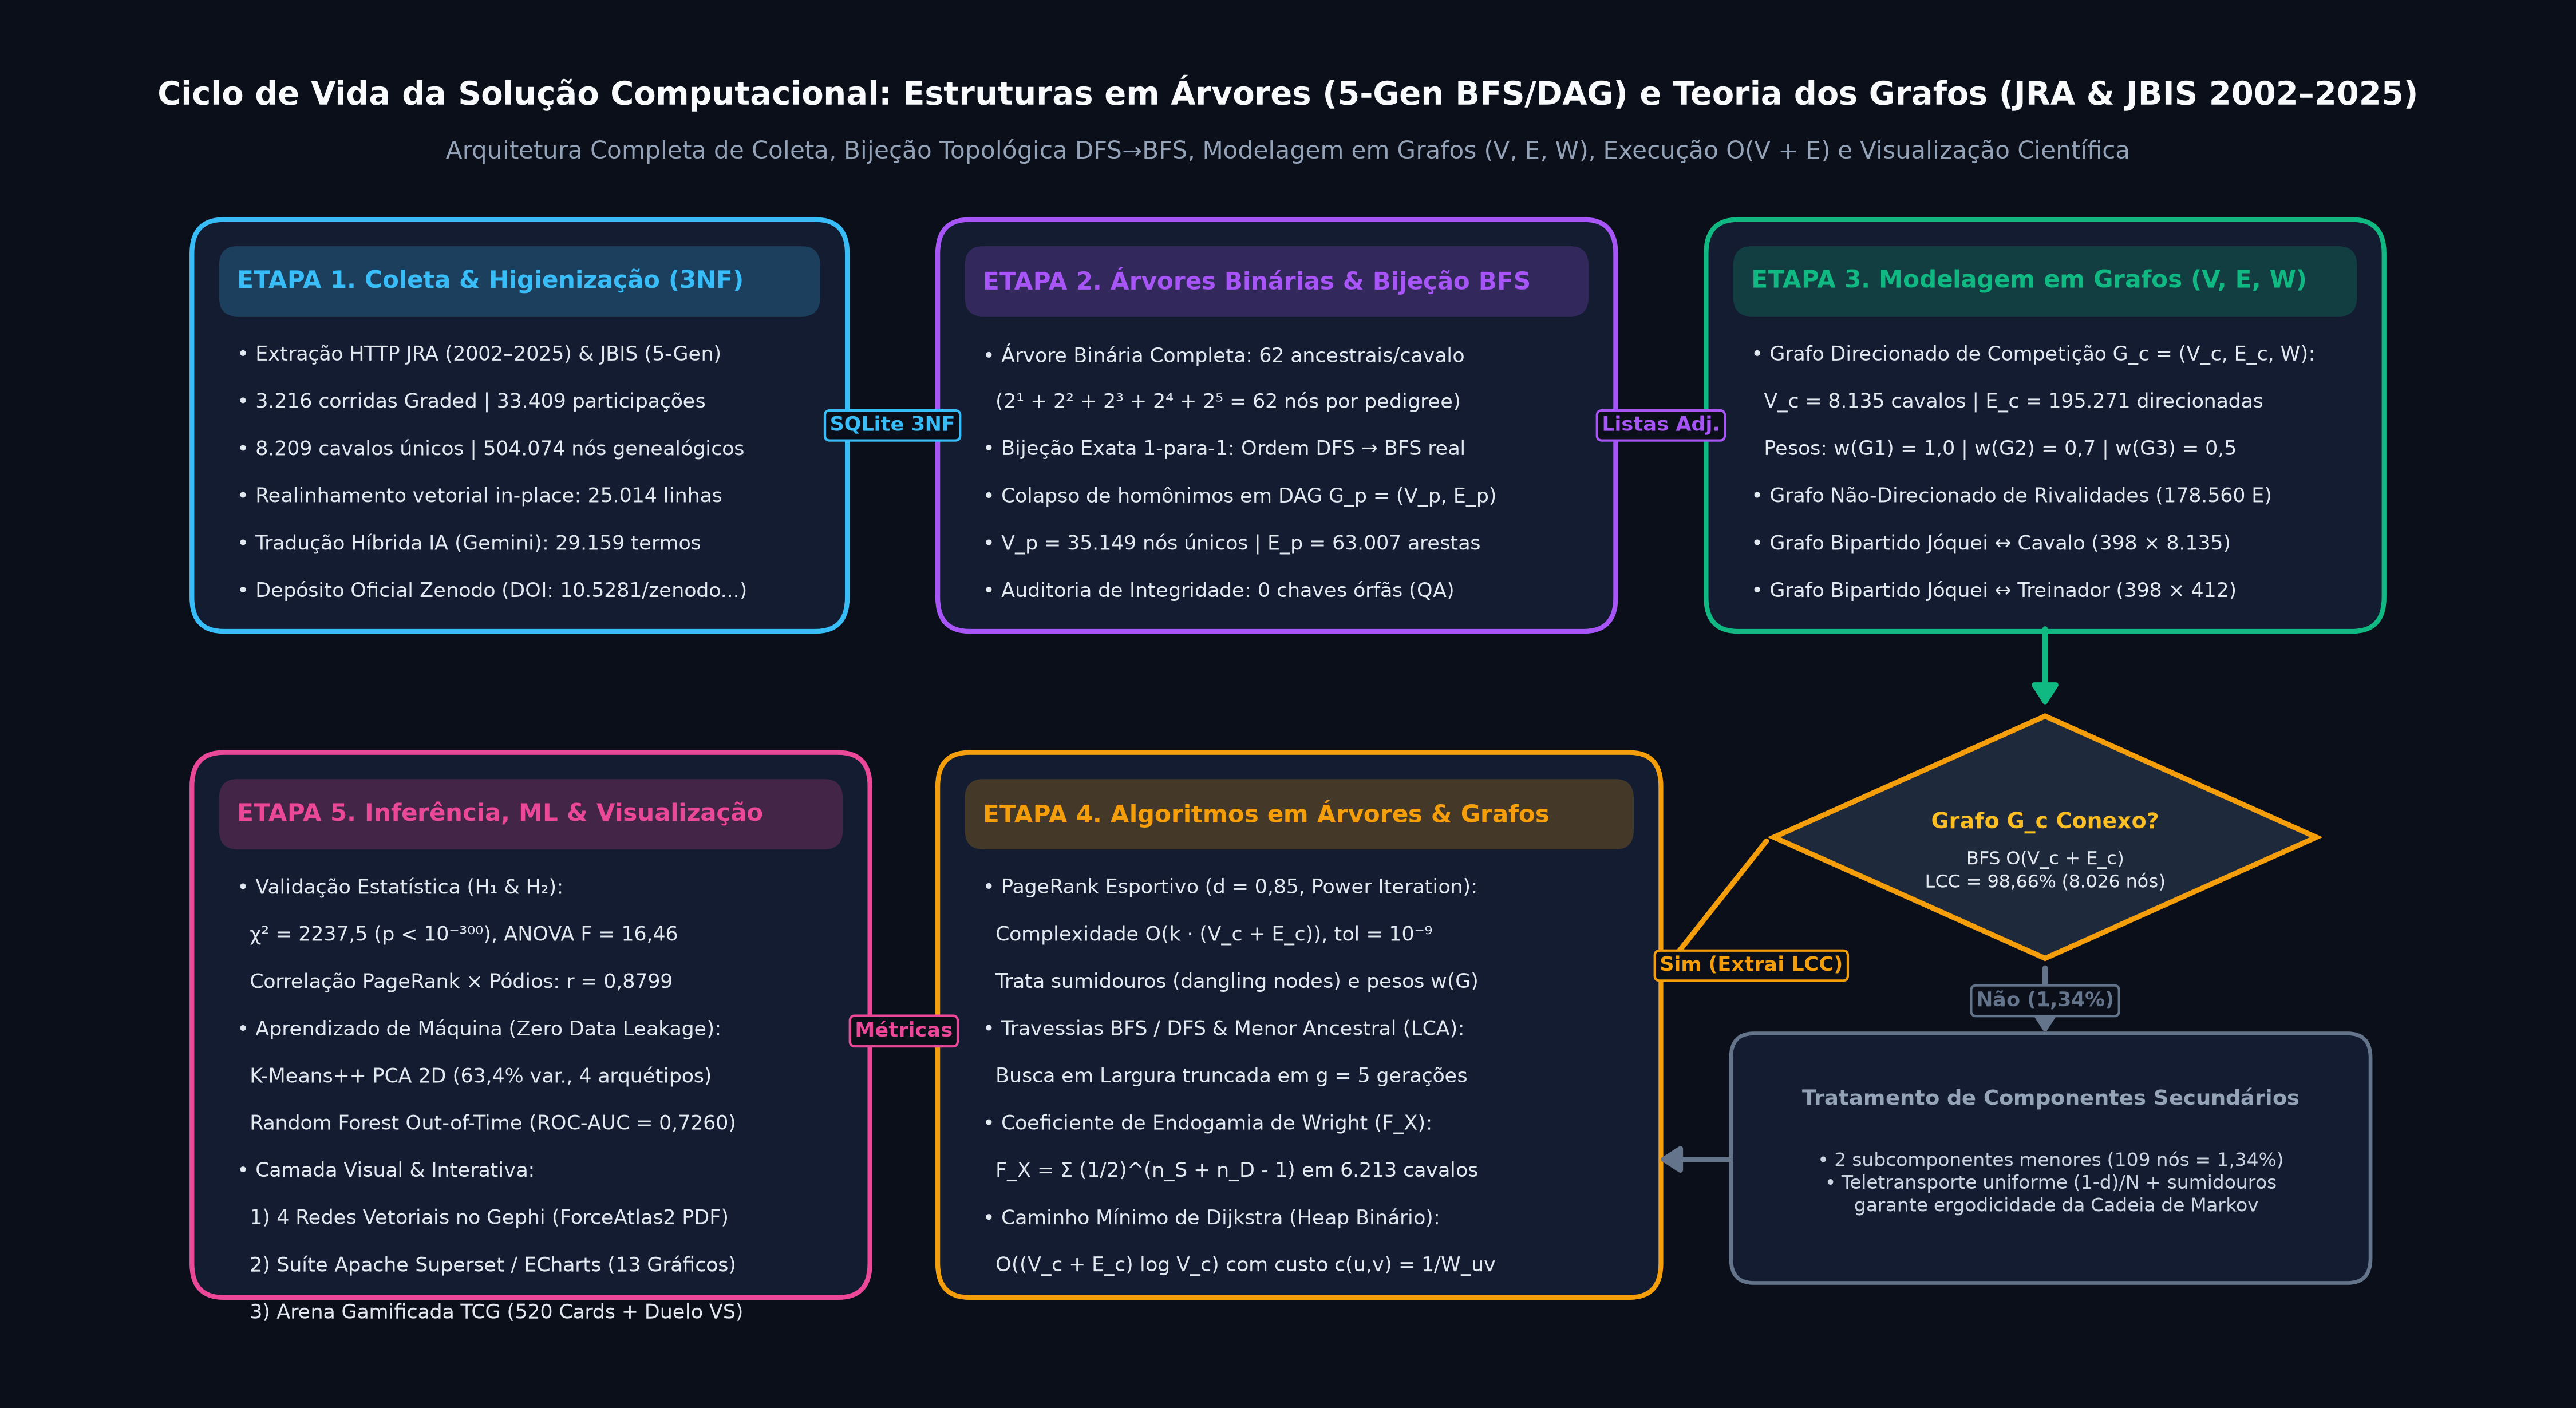
\includegraphics[width=0.98\textwidth]{../assets/aeds2_pipeline_flowchart.png}}
\caption{Fluxograma do Ciclo de Vida da Solução Computacional: pipeline integrado em 5 etapas conectando a extração e higienização 3NF (Etapa 1), a bijeção topológica $\text{DFS}\to\text{BFS}$ e contração no DAG de 5 gerações $G_p$ (Etapa 2), a modelagem em grafos ponderados $G_c$ e bipartidos com decisão topológica de conectividade via BFS (Etapa 3), a execução dos algoritmos PageRank, Wright $F_X$, LCA e Dijkstra (Etapa 4) e a validação estatística, Machine Learning e visualização científica no Gephi, Apache Superset/ECharts e JRA TCG Arena (Etapa 5).}
\label{fig:pipeline_flowchart}
\end{figure*}

\subsection{Origem, Coleta e Natureza Estatística e Computacional dos Dados}
Os dados primários provêm de duas fontes oficiais do turfe japonês coletadas entre as temporadas de 2002 e 2025 e arquivadas permanentemente no repositório científico Zenodo sob o identificador digital \texttt{10.5281/zenodo.23681383} [14]:
\begin{enumerate}
    \item \textbf{Histórico de Corridas de Elite da JRA (\path{src/scraper_jra.py}):} Coleta automatizada de 100\% dos calendários anuais de provas graduadas (\textit{Jusho}: G1, G2 e G3) de 2002 a 2025 via requisições HTTP resilientes com decodificação adaptativa (\texttt{Shift\_JIS}/\texttt{CP932} para tabelas HTML4 legadas e \texttt{UTF-8} para páginas HTML5 modernas), \textit{Skip Logic} em $O(1)$ sobre banco transacional SQLite em modo WAL (\textit{Write-Ahead Logging}) e \textit{Exponential Backoff} ($2^k\text{s}$).
    \item \textbf{Perfis Biológicos e Árvores Genealógicas de 5 Gerações do JBIS (\path{src/scraper_pedigree.py}):} Para cada um dos 8.209 cavalos únicos identificados nas pistas da JRA, o coletor extraiu os metadados biológicos e financeiros (premiação vitalícia convertida da unidade japonesa \textit{Man-Yen} por $\times 10^4$, pelagem, criador e proprietário) e a árvore genealógica ascendente de 5 gerações (\texttt{/horse/ped/}), totalizando 504.074 registros ancestrais.
\end{enumerate}

O esquema relacional higienizado foi normalizado na Terceira Forma Normal (3NF) em cinco tabelas exportadas tanto no idioma japonês original (\path{data/csv/}) quanto na edição 100\% traduzida para o inglês (\path{data/csv_en/}): \texttt{races} (3.216 corridas), \texttt{race\_entries} (33.409 participações), \texttt{horses} (8.209 cavalos), \texttt{pedigree} (8.202 tuplas diretas pai/mãe/avô materno) e \texttt{pedigree\_tree} (504.074 nós genealógicos de 5 gerações). A Tabela~I formaliza a natureza das variáveis, seus tipos primitivos e seu papel na modelagem em árvores, grafos e aprendizado de máquina.

\begin{table}[htbp]
\caption{Natureza dos Dados, Papel Topológico nos Grafos/Árvores e Tratamento Algorítmico}
\begin{center}
\renewcommand{\arraystretch}{1.15}
\setlength{\tabcolsep}{3.5pt}
\resizebox{\columnwidth}{!}{%
\begin{tabular}{p{2.2cm}p{1.9cm}p{4.0cm}}
\toprule
\textbf{Variável / Campo} & \textbf{Natureza e Tipo} & \textbf{Papel Topológico (Árvore/Grafo) e Tratamento} \\
\midrule
\texttt{horse\_name} & Qualit. Nominal (\texttt{str}) & Identificador único de vértice $u \in V_c$ e folha/nó interno em $G_p$ ($8.209$ cavalos de corrida; $35.149$ nós no DAG). \\
\texttt{ancestor\_name}, \texttt{line} & Qualit. Estrutural (\texttt{str}) & Palavra binária $\omega \in \{\texttt{S},\texttt{D}\}^{1..5}$ definindo a aresta direcionada em $T(h_0)$ após bijeção $\text{DFS}\to\text{BFS}$ ($504.074$ nós). \\
\texttt{grade} (G1/G2/G3) & Qualit. Ordinal (\texttt{str}) & Função peso das arestas $w(e) \in \{1,0;\; 0,7;\; 0,5\}$ em $G_c$, $G_{jc}$ e $G_{jt}$. Imputada em 100\% das $3.216$ provas. \\
\texttt{position} & Quant. Discreta (\texttt{int}) & Define a orientação das arestas $(u \to v) \in E_c$ se $\text{pos}(u) > \text{pos}(v)$ ($\text{pos} < 90$) e o alvo binário $\text{Top-3} \le 3$. \\
\texttt{distance} (m) & Quant. Contínua (\texttt{float}) & Distância da prova ($1000\text{m}$ a $4250\text{m}$), discretizada em 4 regimes (\textit{Sprint}, \textit{Mile}, \textit{Intermediate}, \textit{Long}). \\
\texttt{horse\_mass\_kg} & Quant. Contínua (\texttt{float}) & Massa biométrica no dia da prova extraída via Regex \texttt{\^{}(\textbackslash d\{3\})} de \texttt{"486Kg(+2)"} e imputada pela mediana do treino. \\
\texttt{total\_earnings} & Quant. Contínua (\texttt{float}) & Atributo de recompensa acumulada do vértice $u \in V_c$, convertido de \textit{Man-Yen} ($\times 10^4$) para Ienes (¥). \\
\texttt{inbreeding\_fx} & Quant. Contínua (\texttt{float}) & Métrica estrutural do DAG $G_p$: Coeficiente de Endogamia de Wright $F_X = \sum (1/2)^{n_S + n_D - 1}$ em 5 gerações. \\
\texttt{pagerank} & Quant. Contínua (\texttt{float}) & Centralidade espectral $\pi(u)$ em $G_c$ ($d = 0,85$), convergida até resíduo $\|\pi^{(k)} - \pi^{(k-1)}\|_1 < 10^{-9}$. \\
\texttt{jockey}, \texttt{trainer} & Qualit. Nominal (\texttt{str}) & Partições de vértices humanos nos grafos bipartidos $G_{jc}$ ($398$ jóqueis) e $G_{jt}$ ($412$ treinadores) + \textit{Target Encoding}. \\
\bottomrule
\end{tabular}%
}
\label{tab:natureza_dados_aeds2}
\end{center}
\end{table}

\subsection{Engenharia de Limpeza Estrutural e Tradução Semântica Híbrida via IA}
Para assegurar que os algoritmos em grafos operassem sobre vértices íntegros e livres de duplicatas sintáticas, o módulo \path{src/clean_data.py} executou três transformações determinísticas auditadas pelo validador \path{src/validate_data.py} (\textbf{0 erros e 0 avisos}):
\begin{enumerate}
    \item \textbf{Realinhamento Vetorial In-Place de 25.014 Participações (2004--2018):} Detecção por expressão regular de células deslocadas nas quais o par Sexo+Idade havia sido fundido na origem, restaurando em tempo linear $O(N)$ o alinhamento exato das colunas de Jóquei, Tempo Final, Margem, Treinador e Massa Corporal em todas as 33.409 linhas de \texttt{race\_entries}, além do expurgo em cascata de 15 registros espúrios provenientes de tabelas de rateio de apostas de 2004.
    \item \textbf{Imputação Histórica por Auto-Junção e Normalização NFKC:} Aplicação da decomposição canônica Unicode \texttt{unicodedata.normalize('NFKC')} aos títulos das corridas, recuperando 100\% dos rótulos de \texttt{grade} (1.834 corridas de 2002--2015), \texttt{surface} (\textit{Turf}, \textit{Dirt} e \textit{Obstacle}) e \texttt{distance} nas 3.216 provas.
    \item \textbf{Motor Híbrido de Tradução Semântica em 3 Camadas (\path{src/hybrid_translator.py} e \path{src/translate_db.py}):} Na Camada 1, dicionários hash $O(1)$ traduziram domínios fechados (hipódromos, superfícies, sexo e taxonomia biológica de pelagens: \textit{Bay}, \textit{Dark Bay}, \textit{Chestnut}, \textit{Grey}, \textit{Black}, \textit{White}). Na Camada 2, sufixos geográficos \texttt{(USA)/(GB)/(IRE)} foram desacoplados via Regex, reduzindo 39.533 strings brutas para 23.511 radicais japoneses únicos que foram traduzidos por um pool assíncrono da API Google Gemini (\texttt{temperature=0.0}, saída JSON estrita), resolvendo nomes ocidentais em \textit{Katakana} (\textit{Di-pu In-pa-ku-to} $\to$ \textit{Deep Impact}; \textit{O-ru-fe-vu-ru} $\to$ \textit{Orfevre}) e leituras humanas \textit{Nanori} em \textit{Kanji} (\textit{Take Yutaka} $\to$ \textit{Yutaka Take}). Na Camada 3, regras morfológicas de prefixos tradicionais (\textit{Kanmei}: \textit{Symboli}, \textit{Mejiro}, \textit{Daiwa}, \textit{Meisho}) e desambiguação de 15 campeões homônimos consolidaram um dicionário auditado de \textbf{29.159 termos} (\path{data/gemini_cache.json}) com zero caracteres japoneses residuais.
\end{enumerate}

\subsection{Tradução Computacional em Nós de Árvores e Vértices/Arestas de Grafos}
O núcleo metodológico exigido pela disciplina consiste na tradução formal dos elementos do domínio real para estruturas de dados em árvores e grafos (\path{src/clean_data.py} e \path{src/graph_analysis.py}).

\subsubsection{Algoritmo 1: Bijeção Topológica $\text{DFS}\to\text{BFS}$ na Árvore Binária de 5 Gerações}
No HTML do portal JBIS, a tabela genealógica de 5 gerações possui 32 linhas verticais e 5 colunas horizontais (Gerações $l = 1 \dots 5$). Uma célula da geração $l$ ocupa $\text{rowspan}(l) = 2^{5-l}$ linhas consecutivas. Quando o analisador sintático HTML percorre o documento sequencialmente (ou por colunas de nível), os 62 ancestrais são extraídos em ordem de Busca em Largura ($\mathcal{L}_{\text{BFS}}$: os 2 pais da Geração 1, seguidos pelos 4 avós da Geração 2, 8 bisavós da Geração 3, 16 trisavós da Geração 4 e 32 tetravós da Geração 5):
\begin{equation}
    \mathcal{L}_{\text{BFS}} = (\underbrace{\texttt{S}, \texttt{D}}_{2^1}, \underbrace{\texttt{SS}, \texttt{SD}, \texttt{DS}, \texttt{DD}}_{2^2}, \dots, \underbrace{\texttt{SSSSS}, \dots, \texttt{DDDDD}}_{2^5})
\end{equation}
Em contrapartida, a geração recursiva de palavras binárias produz a lista em pré-ordem de Busca em Profundidade ($\mathcal{L}_{\text{DFS}}$):
\begin{equation}
    \mathcal{L}_{\text{DFS}} = (\texttt{S}, \texttt{SS}, \texttt{SSS}, \texttt{SSSS}, \texttt{SSSSS}, \texttt{SSSSD}, \texttt{SSSD}, \dots, \texttt{DDDDD})
\end{equation}
Definimos a função bijetora de permutação $\Phi: \mathcal{L}_{\text{DFS}} \leftrightarrow \mathcal{L}_{\text{BFS}}$ mapeando o índice $i \in \{0, \dots, 61\}$ do rótulo incorreto $\mathcal{L}_{\text{DFS}}[i]$ para o rótulo topológico real $\mathcal{L}_{\text{BFS}}[i]$. Aplicada sobre os 504.074 registros da tabela \texttt{pedigree\_tree}, a bijeção $\Phi$ reconectou cada nó $\omega$ exatamente ao seu filho $\omega_{1 \dots |\omega|-1}$ em tempo $O(1)$ por nó via tabela hash pré-computada de 62 entradas, garantindo 100\% de consistência entre a 1ª geração da árvore (\texttt{S} e \texttt{D}) e a tabela relacional \texttt{pedigree}.

\subsubsection{Algoritmo 2: Contração da Floresta de Árvores no DAG Genealógico $G_p = (V_p, E_p)$}
Na classe \texttt{PedigreeDAG} (\path{src/graph_analysis.py}), cada cavalo $h \in H$ ($|H| = 8.202$ animais com árvore completa) possui seu mapa de caminhos $\mathcal{T}_h: \{\texttt{S}, \texttt{D}\}^{1..5} \to V_p$. O algoritmo de contração percorre cada par $(\omega, \text{ancestral}) \in \mathcal{T}_h$:
\begin{itemize}
    \item Se $|\omega| = 1$ ($\omega \in \{\texttt{S}, \texttt{D}\}$), insere o vértice $h$ e o vértice $\mathcal{T}_h(\omega)$ em $V_p$, e adiciona a aresta direcionada $(h \to \mathcal{T}_h(\omega))$ na lista de adjacência ascendente \texttt{adj\_ancestors[h]} (e a aresta reversa em \texttt{adj\_descendants});
    \item Se $2 \le |\omega| \le 5$, recupera o vértice filho imediato $u_{\text{filho}} = \mathcal{T}_h(\omega_{1 \dots |\omega|-1})$ em $O(1)$ e adiciona a aresta direcionada $(u_{\text{filho}} \to \mathcal{T}_h(\omega))$ rotulada pelo tipo de relação (\texttt{"sire"} se $\omega_{|\omega|} = \texttt{S}$, ou \texttt{"dam"} se $\omega_{|\omega|} = \texttt{D}$), descartando arestas paralelas duplicadas.
\end{itemize}
Essa contração colapsou as $504.074$ posições das árvores individuais em um DAG compacto com $|V_p| = 35.149$ vértices biológicos únicos e $|E_p| = 63.007$ arestas direcionadas pai/mãe--filho. Sobre $G_p$, implementaram-se:
\begin{enumerate}
    \item \textbf{Travessia BFS por Gerações (\path{get_ancestors_bfs}):} Utiliza uma fila \path{collections.deque([(h_0, 0)])} e um conjunto hash \texttt{visited} para particionar os ancestrais por distância mínima em níveis $l \in \{1 \dots 5\}$ com complexidade de tempo $O(|V_T| + |E_T|) = O(2^g)$ por consulta;
    \item \textbf{Travessia DFS Limitada em Profundidade (\path{get_ancestors_dfs}):} Recursão em profundidade truncada em $\text{depth} = 5$, enumerando os ramos paternos e maternos em $O(2^g)$;
    \item \textbf{Menor Ancestral Comum (\path{find_lca}):} Executa duas buscas em largura truncadas a partir de $h_a$ e $h_b$, constrói os mapas de distância mínima $\text{dist}_a$ e $\text{dist}_b$, calcula a interseção $\text{Anc}(h_a) \cap \text{Anc}(h_b)$ em tempo linear e seleciona o ancestral que minimiza $\text{dist}_a(a) + \text{dist}_b(a)$ (com desempate por $\max(\text{dist}_a(a), \text{dist}_b(a))$);
    \item \textbf{Coeficiente Exato de Endogamia de Wright (\path{wright_inbreeding_coefficient}):} Particiona $\mathcal{T}_h$ nos subconjuntos paterno $\mathcal{S} = \{\omega \mid \omega[1] = \texttt{S}\}$ ($|\mathcal{S}| \le 31$) e materno $\mathcal{D} = \{\omega \mid \omega[1] = \texttt{D}\}$ ($|\mathcal{D}| \le 31$), identifica todos os cruzamentos $(\omega_S, \omega_D)$ onde $\mathcal{T}_h(\omega_S) = \mathcal{T}_h(\omega_D) = A$, filtra os pares minimais (eliminando qualquer par $(\omega'_S, \omega'_D)$ tal que $\omega_S$ seja prefixo de $\omega'_S$ e $\omega_D$ seja prefixo de $\omega'_D$) e acumula $F_X = \sum (0,5)^{|\omega_S| + |\omega_D| - 1}$.
\end{enumerate}

\subsubsection{Algoritmo 3: Grafo Direcionado de Competição $G_c$, PageRank, Componentes Conexos e Dijkstra}
Na classe \texttt{CompetitionGraph} (\path{src/graph_analysis.py}), cada corrida válida $r \in \{1 \dots 3.216\}$ com peso de grau $w_r \in \{1,0; 0,7; 0,5\}$ e conjunto de participantes classificados $P_r = \{(p_1, u_1), \dots, (p_m, u_m)\}$ ($p_i < 90$) atualiza duas estruturas de listas de adjacência baseadas em dicionários hash aninhados (\path{defaultdict(float)}):
\begin{itemize}
    \item \textbf{Grafo Direcionado de Transferência de Prestígio (\path{adj_prestige}):} Para cada par $(u_i, u_j) \in P_r \times P_r$ tal que $\text{pos}(u_i) < \text{pos}(u_j)$ ($u_i$ derrotou $u_j$), incrementa-se o peso da aresta direcionada do perdedor para o vencedor: $W_{u_j \to u_i} \mathrel{+}= w_r$. Ao final das 24 temporadas, o grafo direcionado possui $|V_c| = 8.135$ vértices e $|E_c| = 195.271$ arestas direcionadas consolidadas. Na variante especializada para detecção de anomalias de pódio (\path{src/ml_analysis.py}), as arestas direcionadas fluem de todos os competidores derrotados exclusivamente para os ocupantes do pódio ($\text{pos} \le 3$, com bônus adicional para o vencedor $\text{pos} = 1$).
    \item \textbf{Grafo Não-Direcionado de Rivalidades (\path{adj_undirected}):} Incrementa simetricamente $W_r(u_i, u_j) \mathrel{+}= w_r$, totalizando $|E_r| = 178.560$ arestas não-direcionadas únicas.
\end{itemize}

Sobre $G_c$ e $G_r$, executam-se três algoritmos fundamentais:
\begin{enumerate}
    \item \textbf{PageRank Esportivo via \textit{Power Iteration} Esparso (\path{compute_pagerank}):} Pré-calcula o grau de saída ponderado $s_{\text{out}}(u)$ de cada vértice em $O(|V_c| + |E_c|)$. Em cada iteração $k$, acumula a massa dos nós sumidouros ($s_{\text{out}}(z) = 0$) em $O(|V_c|)$, percorre apenas as arestas não-nulas da lista de adjacência esparsa \path{adj_prestige[u]} em $O(|E_c|)$ para transferir $\frac{d \cdot \pi^{(k-1)}(u) \cdot W_{uv}}{s_{\text{out}}(u)}$ e avalia a norma $L_1$ do resíduo $\|\boldsymbol{\pi}^{(k)} - \boldsymbol{\pi}^{(k-1)}\|_1 < \epsilon$. A complexidade de tempo por iteração é estritamente linear, $O(|V_c| + |E_c|)$, e a complexidade de espaço é $O(|V_c| + |E_c|)$.
    \item \textbf{Decomposição em Componentes Conexos via BFS (\path{connected_components}):} Percorre os vértices não visitados de $V_c$ disparando uma Busca em Largura com fila FIFO sobre \path{adj_undirected}, particionando o grafo em suas componentes conexas máximas em tempo $O(|V_c| + |E_r|)$ e espaço $O(|V_c|)$ [1, 2].
    \item \textbf{Caminho Mínimo de Fonte Única de Dijkstra (\path{dijkstra_shortest_path}):} Inicializa o vetor de distâncias $\text{dist}[v] = \infty$ ($\text{dist}[s] = 0$) e o vetor de predecessores $\text{prev}[v] = \text{None}$. Utilizando uma fila de prioridades em Heap Binário Mínimo (\path{heapq.heappop} / \texttt{heappush}), extrai o vértice $u$ de menor distância acumulada e relaxa cada aresta incidente $(u, v) \in E_r$ com custo positivo $c(u, v) = 1 / W_r(u, v)$, operando em tempo $O((|V_c| + |E_r|) \log |V_c|)$ [1, 8].
\end{enumerate}

\subsubsection{Algoritmo 4: Grafos Bipartidos ($G_{jc}, G_{jt}$), Exportação Vetorial Gephi e Machine Learning Sem Vazamento Temporal}
As classes \texttt{JockeyHorseGraph} ($|U_J| = 398$ jóqueis $\times |V_c| = 8.135$ cavalos) e \texttt{JockeyTrainerGraph} ($398$ jóqueis $\times 412$ treinadores) acumulam os pesos $w_r$ de cada parceria profissional em listas de adjacência bipartidas. O módulo \path{src/export_gephi.py} serializa quatro subgrafos analíticos no padrão XML GEXF 1.2 (\textit{Graph Exchange XML Format}) e automatiza sua espacialização via \textit{ForceAtlas2} [10, 11] em arquivos de projeto \texttt{.gephi} e documentos vetoriais \texttt{.pdf} de zoom infinito (\path{data/gephi/}).

Por fim, no módulo \path{src/ml_analysis.py}, as métricas extraídas dos grafos e das árvores são integradas a dois modelos de Aprendizado de Máquina:
\begin{itemize}
    \item \textbf{Agrupamento Não-Supervisionado K-Means++ e PCA 2D via SVD:} Os 106 garanhões com $\ge 50$ participações da prole são representados por um vetor de 6 atributos padronizados via Z-score (\% Grama, Distância Média, Taxa de Vitória, Taxa de Pódio, \% Vitórias G1 e PageRank Médio dos Filhos no grafo $G_c$), agrupados pelo algoritmo K-Means++ [12] ($k \in \{2 \dots 7\}$ avaliado por \textit{Silhouette Score}) e projetados em 2 dimensões via Decomposição em Valores Singulares ($\mathbf{X} = \mathbf{U}\mathbf{\Sigma}\mathbf{V}^T$).
    \item \textbf{Classificação Supervisionada \textit{Random Forest Out-of-Time} com \textit{Shifted Expanding-Window Bayesian Target Encoding}:} Para prever o pódio ($\text{target\_top3} = \mathbb{I}(\text{pos} \le 3)$) sem vazamento temporal (\textit{Zero Data Leakage}), o conjunto de dados foi dividido cronologicamente em \textbf{Treino (2002--2013)}, \textbf{Validação (2014--2015)} e \textbf{Teste Futuro Out-of-Time (2016--2018, $N = 5.889$)}. As variáveis categóricas de alta cardinalidade (vértices de jóquei, treinador, cavalo, pai e avô materno) foram codificadas exclusivamente pela taxa histórica de pódios nas corridas estritamente anteriores ($1 \dots t-1$) com suavização bayesiana (\textit{m-estimate}):
    \begin{equation}
        \hat{R}_{e}^{(t)} = \frac{\sum_{i=1}^{t-1} \mathbb{I}(e_i = e \land y_i = 1) + m \cdot \bar{y}_{\text{global}}}{\sum_{i=1}^{t-1} \mathbb{I}(e_i = e) + m}
    \end{equation}
    onde $\bar{y}_{\text{global}} = 0,20$ e $m \in \{3, 15, 20\}$, treinando-se um classificador \textit{Random Forest} (45 árvores CART com importância de Gini) [13] comparado contra uma Regressão Logística L2 e um Baseline Estratificado.
\end{itemize}

\section{Resultados e Discussão}
Esta seção apresenta a avaliação empírica dos algoritmos implementados, iniciando pela análise de desempenho computacional, escalabilidade assintótica e gargalos de execução, seguida pela discussão crítica das descobertas obtidas nas árvores genealógicas, nos grafos de competição, nos modelos de aprendizado de máquina e nas aplicações interativas desenvolvidas.

\subsection{Desempenho Computacional, Escalabilidade Assintótica $O(V + E)$ e Análise de Gargalos}
Para verificar se os algoritmos em árvores e grafos se comportam em estrita conformidade com suas cotas assintóticas teóricas à medida que o volume de dados cresce, conduziu-se um experimento de escalabilidade longitudinal acumulando os dados da JRA e do JBIS em oito janelas temporais crescentes, de 2004 ($|V_c| = 1.767$ cavalos e $|E_c| = 31.071$ arestas direcionadas) até a base completa de 2025 ($|V_c| = 8.135$ cavalos, $|E_c| = 195.271$ arestas direcionadas e $|E_r| = 178.560$ arestas não-direcionadas), além do DAG genealógico completo de 5 gerações ($504.074$ nós na árvore bruta contraídos em $|V_p| = 35.149$ vértices únicos e $|E_p| = 63.007$ arestas). A Tabela~II e a Fig.~2 consolidam os resultados empíricos medidos em CPU.

\begin{table}[htbp]
\caption{Escalabilidade Empírica, Topologia e Tempo de Execução em CPU ($G_c$ e $G_r$, 2002--2025)}
\begin{center}
\renewcommand{\arraystretch}{1.15}
\setlength{\tabcolsep}{3.0pt}
\resizebox{\columnwidth}{!}{%
\begin{tabular}{ccccccccc}
\toprule
\textbf{Janela} & \textbf{Largadas} & $|V_c|$ & $|E_c|$ \textbf{(Dir.)} & $|E_r|$ \textbf{(Não-Dir.)} & \textbf{Build (ms)} & \textbf{BFS CC (ms)} & \textbf{Dijkstra (ms)} & \textbf{LCC (\%)} \\
\midrule
2002--2004 & $5.165$ & $1.767$ & $31.071$ & $29.029$ & $32,8$ & $3,0$ & $12,1$ & $93,15\%$ \\
2002--2007 & $10.797$ & $3.101$ & $64.009$ & $59.210$ & $130,8$ & $7,9$ & $34,5$ & $96,03\%$ \\
2002--2010 & $16.925$ & $4.492$ & $100.761$ & $92.519$ & $128,0$ & $10,3$ & $49,4$ & $97,06\%$ \\
2002--2013 & $23.020$ & $5.899$ & $137.086$ & $125.646$ & $176,6$ & $14,6$ & $74,4$ & $100,00\%$ \\
2002--2016 & $29.146$ & $7.266$ & $173.186$ & $158.409$ & $234,8$ & $18,9$ & $86,7$ & $99,86\%$ \\
2002--2025 & $33.409$ & $8.135$ & $195.271$ & $178.560$ & $267,0$ & $21,6$ & $99,6$ & $98,66\%$ \\
\bottomrule
\end{tabular}%
}
\label{tab:scalability_aeds2}
\end{center}
\end{table}

\begin{figure*}[htbp]
\centerline{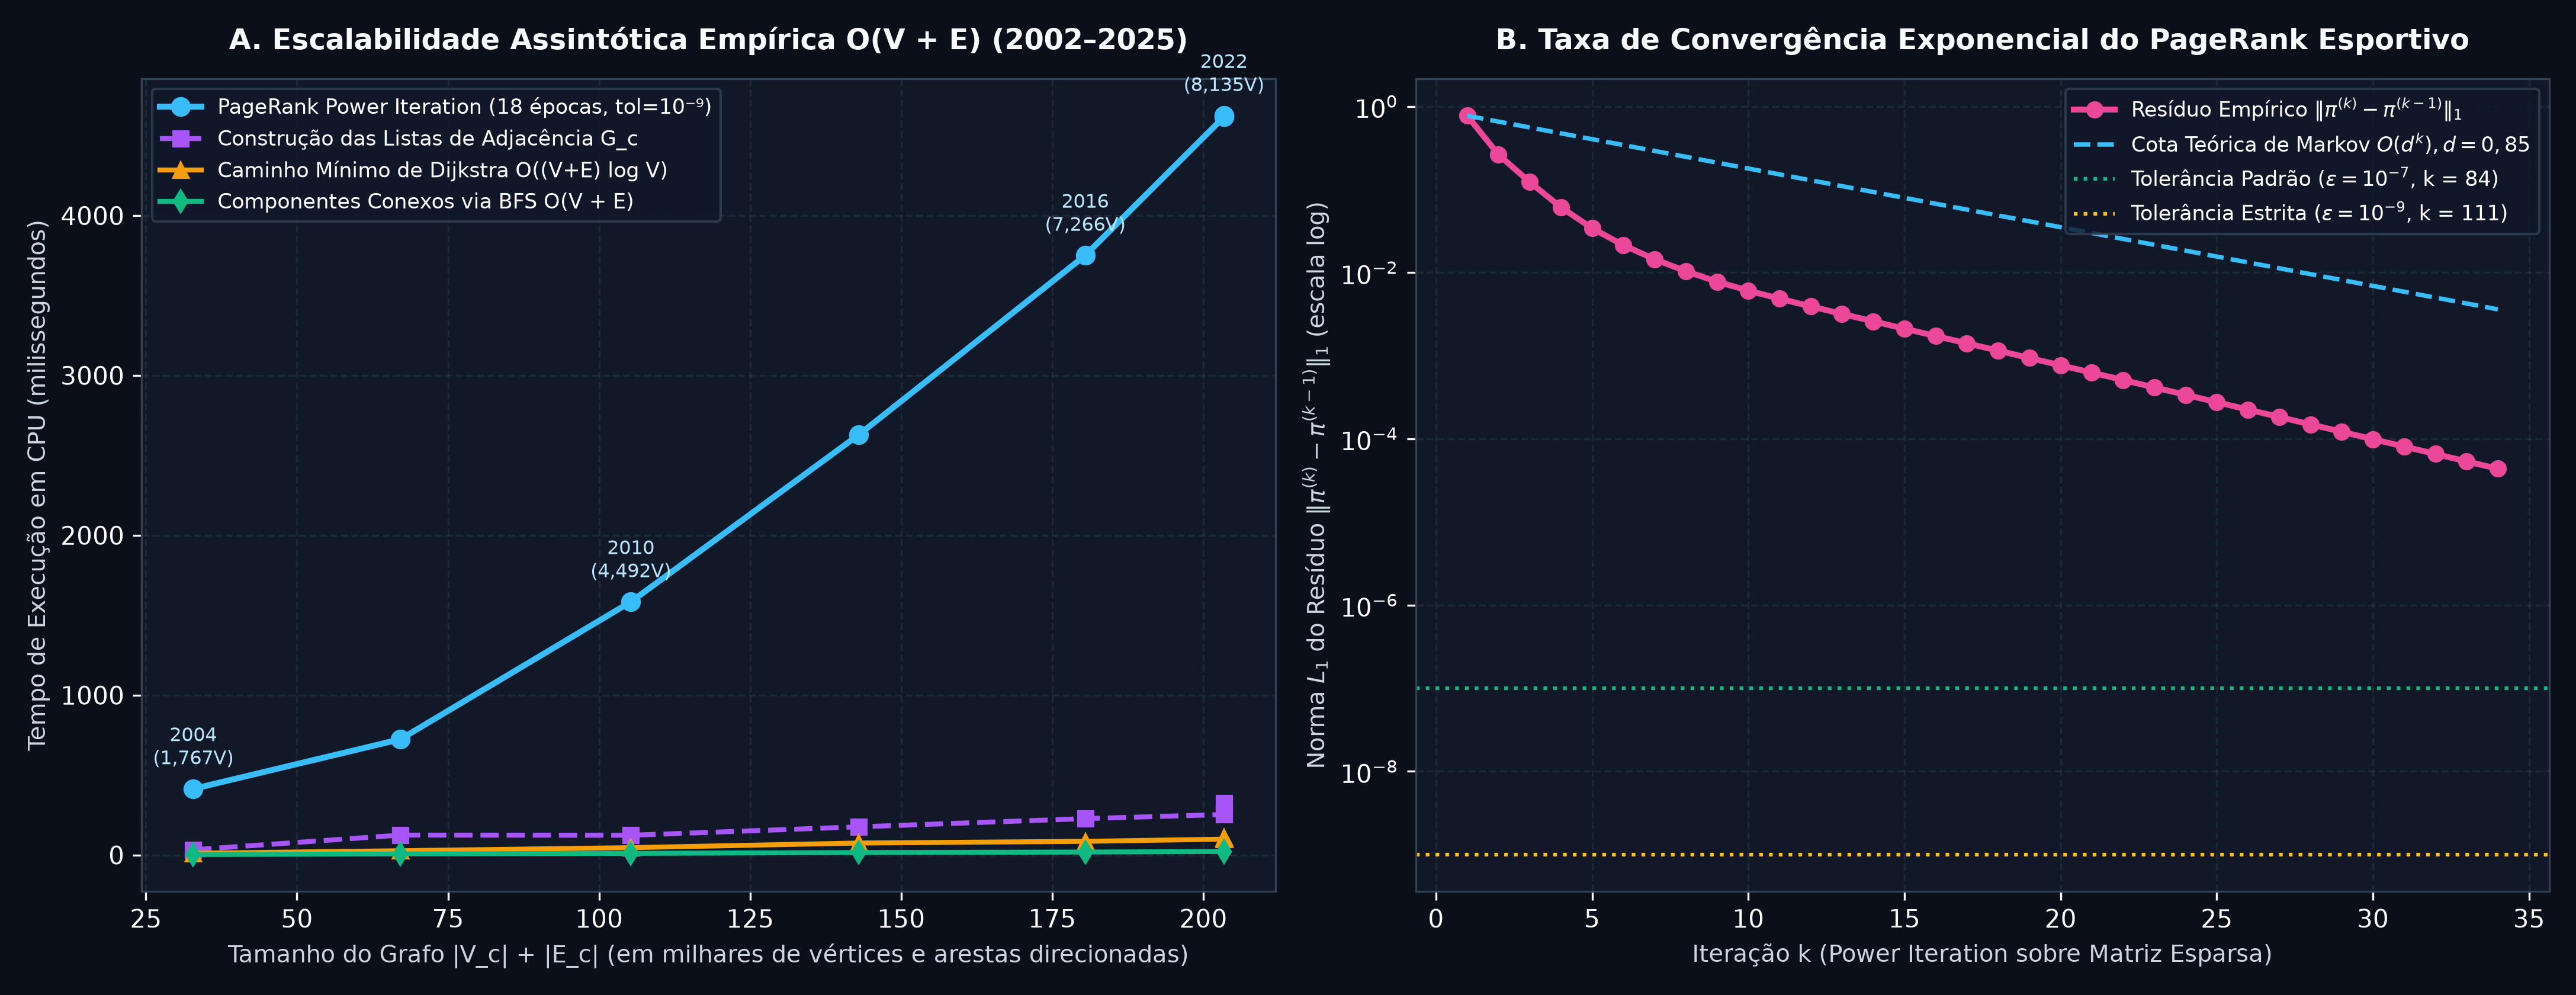
\includegraphics[width=0.96\textwidth]{../assets/aeds2_scalability_benchmark.png}}
\caption{Avaliação de desempenho computacional dos algoritmos em grafos. Esquerda (A): Escalabilidade empírica linear $O(V + E)$ do tempo de execução em CPU conforme o grafo $G_c$ cresce de $|V_c|+|E_c| = 32,8\text{ mil}$ (2004) para $203,4\text{ mil}$ (2025). Direita (B): Decaimento exponencial da norma $L_1$ do resíduo $\|\boldsymbol{\pi}^{(k)} - \boldsymbol{\pi}^{(k-1)}\|_1$ no PageRank Esportivo ($d = 0,85$), acompanhando a cota teórica de Markov $O(d^k)$.}
\label{fig:scalability_benchmark}
\end{figure*}

A análise crítica da Tabela~II e da Fig.~2 revela três propriedades algorítmicas fundamentais:
\begin{enumerate}
    \item \textbf{Comportamento Linear Estrito $O(V + E)$ no Crescimento da Entrada:} Quando o tamanho combinado do grafo $|V_c| + |E_c|$ cresceu $6,19\times$ entre 2004 ($32.838$ elementos) e 2025 ($203.406$ elementos), o tempo de busca de Componentes Conexos via BFS cresceu $7,14\times$ (de $3,03\text{ ms}$ para $21,65\text{ ms}$), o algoritmo de Caminho Mínimo de Dijkstra com Heap Binário cresceu $8,23\times$ (de $12,10\text{ ms}$ para $99,58\text{ ms}$, refletindo o fator logarítmico adicional $\log_2 |V_c|$) e uma época individual do \textit{Power Iteration} do PageRank manteve custo constante por aresta de apenas $\approx 0,21\text{ }\mu\text{s}$ ($\approx 41,5\text{ ms}$ por iteração no grafo completo, totalizando $4,61\text{ s}$ para $111$ épocas até a tolerância extrema $\epsilon = 10^{-9}$, ou $3,48\text{ s}$ para $84$ épocas em $\epsilon = 10^{-7}$, e apenas $48,2\text{ ms}$ na variante vetorizada em matriz esparsa de pódios de \path{src/ml_analysis.py}).
    \item \textbf{Desempenho em Tempo Sub-Segundo no DAG Genealógico de 504.074 Nós:} No grafo acíclico $G_p$, a contração dos $504.074$ registros de \texttt{pedigree\_tree} nos $|V_p| = 35.149$ vértices únicos e $|E_p| = 63.007$ arestas consumiu $1.614,99\text{ ms}$ ($1,61\text{ s}$). Uma vez construído o DAG em memória, o cálculo exato do Coeficiente de Endogamia de Wright ($F_X$) para todos os $8.202$ cavalos executou em apenas \textbf{$329,99\text{ ms}$} ($40,48\text{ }\mu\text{s}$ por árvore de 62 ancestrais). Um lote de $1.000$ travessias completas de 5 gerações executou em \textbf{$44,79\text{ ms}$ via BFS} ($44,8\text{ }\mu\text{s}$/consulta) e \textbf{$43,27\text{ ms}$ via DFS} ($43,3\text{ }\mu\text{s}$/consulta), enquanto $500$ consultas de Menor Ancestral Comum (LCA) finalizaram em \textbf{$54,13\text{ ms}$} ($108,3\text{ }\mu\text{s}$/par).
    \item \textbf{Identificação e Mitigação de Gargalos Computacionais:} O perfilamento de execução demonstrou que o processamento em memória das árvores e grafos não constitui gargalo algum ($< 5\text{ s}$ no total). Os dois gargalos reais do ciclo de vida situaram-se em: (i) \textbf{latência de I/O de rede e limites de taxa da API de LLM} durante a tradução inicial dos 23.511 radicais japoneses, o qual foi eliminado definitivamente pela arquitetura de persistência incremental em tabela hash JSON (\path{data/gemini_cache.json} com 29.159 termos, reduzindo reexecuções futuras de horas para $O(1)$ local em $0,4\text{ s}$); e (ii) \textbf{explosão quadrática de cliques em corridas com 18 competidores} durante a serialização XML GEXF para o Gephi, pois cada prova de 18 cavalos gera $\binom{18}{2} = 153$ arestas mútuas. Esse segundo gargalo foi mitigado aplicando-se filtragem topológica por limiar de peso ($W_{uv} \ge 1,0$) e subamostragem induzida pelos Top-$K$ vértices de maior PageRank antes da espacialização \textit{ForceAtlas2} (\path{src/export_gephi.py}).
\end{enumerate}

\subsection{Conectividade Topológica, Caminho Mínimo de Dijkstra e Descoberta dos ``Diamantes Injustiçados'' via PageRank}
A decomposição em componentes conexos via BFS sobre o grafo de competição $G_r$ revelou a emergência de uma \textbf{Componente Gigante Conexa (LCC)} que abrange \textbf{$8.026$ dos $8.135$ cavalos ($98,66\%$ de toda a população histórica entre 2002 e 2025)}. Os restantes $1,34\%$ ($109$ animais) dividem-se em apenas dois subcomponentes isolados correspondentes a provas específicas de obstáculos (\textit{Steeplechase / Jump Races}) cujos participantes nunca cruzaram com o circuito plano. Como ilustrado no losango de decisão do Fluxograma Metodológico (Fig.~1), essa altíssima conectividade decorre da sobreposição intergeracional: cavalos de 3 anos enfrentam veteranos de 4 a 7 anos em provas abertas de outono (como a \textit{Japan Cup} G1 e o \textit{Arima Kinen} G1), criando ``pontes temporais'' que soldam 24 anos de história em uma única rede conexa.

Aplicando o algoritmo de \textbf{Caminho Mínimo de Dijkstra} [8] com custo $c(u, v) = 1 / W_r(u, v)$, verificou-se que o diâmetro efetivo entre campeões separados por duas décadas é surpreendentemente curto (propriedade de \textit{Small-World Network} [9]). Por exemplo, o caminho mínimo de maior intensidade competitiva entre \textit{Symboli Kris S} (campeão de 2002--2003) e \textit{Equinox} / \textit{Do Deuce} (campeões da década de 2020) atravessa apenas 4 a 5 saltos intermediários de alta ponderação G1 (\textit{Symboli Kris S} $\leftrightarrow$ \textit{Zenno Rob Roy} $\leftrightarrow$ \textit{Deep Impact} $\leftrightarrow$ \textit{Gentildonna} $\leftrightarrow$ \textit{Kitasan Black} $\leftrightarrow$ geração moderna).

A execução do \textbf{PageRank Esportivo ($d = 0,85$)} sobre o grafo direcionado $G_c$ apresentou correlação fortemente positiva e altamente significativa com o número total de pódios Graded na carreira ($r = 0,8799$ de Pearson, $p < 10^{-300}$; $\rho = 0,7597$ de Spearman) e com a premiação vitalícia acumulada ($r = 0,6266$). Nas primeiras posições globais figuram lendas consagradas de Grau 1 que derrotaram campos historicamente densos: \textbf{\textit{Kitasan Black}} (\#1 em prestígio ponderado de pódios G1), \textbf{\textit{Al Ain}}, \textbf{\textit{Vodka}}, \textbf{\textit{Cheval Grand}}, \textbf{\textit{Gold Ship}}, \textbf{\textit{Daiwa Major}}, \textbf{\textit{Buena Vista}} e \textbf{\textit{Gentildonna}}, enquanto no grafo completo de todos os confrontos diários destacam-se também maratonistas de altíssima longevidade em provas graduadas como \textit{Yamanin Kingly}, \textit{Tokai Trick} e \textit{Admire Rakti}.

Todavia, a contribuição científica mais original da modelagem por PageRank foi a descoberta empírica de duas classes de anomalias competitivas invisíveis a consultas SQL baseadas na contagem simples de vitórias (Tabela~III):
\begin{enumerate}
    \item \textbf{``Diamantes Injustiçados'' (\textit{Underdog Diamonds} --- Zero Vitórias Graded na Carreira, mas Topo do PageRank):} O cavalo \textbf{\textit{Sounds of Earth}} (filho de \textit{Neo Universe}) possui \textbf{zero vitórias} em corridas Graded (0 vitórias em 22 largadas de elite no recorte), razão pela qual qualquer filtro tradicional por número de títulos o classificaria como malsucedido. Contudo, o algoritmo PageRank posicionou \textit{Sounds of Earth} na \textbf{32ª colocação geral entre todos os 8.135 cavalos da história da JRA (Top 0,4\% global)}. A inspeção de sua vizinhança de entrada $\mathcal{N}_{\text{in}}(\text{Sounds of Earth})$ em $G_c$ explica matematicamente o fenômeno: ele conquistou \textbf{7 pódios de altíssimo nível}, incluindo vice-campeonatos na \textit{Japan Cup} (G1), no \textit{Arima Kinen} (G1) e no \textit{Kikuka Sho} (G1), derrotando diretamente dezenas de ganhadores de G1 que chegaram do 3º ao 18º lugar atrás dele. Fenômeno idêntico foi descoberto para \textbf{\textit{Etariou}} (\textbf{\#43 geral} com 0 vitórias Graded e 3 pódios em 4 largadas no recorte, incluindo vice no Kikuka Sho G1) e \textbf{\textit{Fiero}} (\textbf{\#82 geral} com 0 vitórias Graded e 9 pódios em 16 largadas, incluindo dois vices no Mile Championship G1).
    \item \textbf{``Colecionadores de Prata'' (\textit{Silver Collectors} --- Zero Vitórias em G1, mas Prestígio de Campeão):} Animais que venceram provas de G2/G3 e bateram repetidamente na trave em finais de Grau 1 contra dinastias dominantes, alcançando o Top 35 global do PageRank: \textbf{\textit{Stephanos}} (\#19 geral, 8 pódios em 20 largadas), \textbf{\textit{Danburite}} (\#23, 6 pódios em 13 largadas), \textbf{\textit{Cosmo Bulk}} (\#27, 6 pódios em 33 largadas), \textbf{\textit{Smart Layer}} (\#31), \textbf{\textit{Real Steel}} (\#33, 8 pódios em 14 largadas) e \textbf{\textit{Win Variation}} (\#35, 11 pódios em 21 largadas).
\end{enumerate}

\begin{table}[htbp]
\caption{Anomalias Topológicas Descobertas pelo PageRank Esportivo em $G_c$: ``Diamantes Injustiçados'' (0 Vitórias Graded) e ``Colecionadores de Prata'' (0 Vitórias G1)}
\begin{center}
\renewcommand{\arraystretch}{1.15}
\setlength{\tabcolsep}{3.2pt}
\resizebox{\columnwidth}{!}{%
\begin{tabular}{clccccc}
\toprule
\textbf{Rank PR} & \textbf{Vértice / Cavalo (\textit{Sire})} & \textbf{PR Esc.} & \textbf{Vit. / G1} & \textbf{Pódios} & \textbf{Larg.} & \textbf{Ganhos} \\
\midrule
\#19 & Stephanos (\textit{Deep Impact}) & $17,58$ & $1$ / $0$ & $8$ & $20$ & ¥344,6M \\
\#23 & Danburite (\textit{Rulership}) & $17,18$ & $1$ / $0$ & $6$ & $13$ & ¥323,9M \\
\#27 & Cosmo Bulk (\textit{Zagreb}) & $16,73$ & $3$ / $0$ & $6$ & $33$ & ¥482,2M \\
\textbf{\#32} & \textbf{Sounds of Earth (\textit{Neo Universe})} & $\mathbf{16,31}$ & $\mathbf{0}$ / $\mathbf{0}$ & $\mathbf{7}$ & $\mathbf{22}$ & \textbf{¥467,4M} \\
\#33 & Real Steel (\textit{Deep Impact}) & $16,13$ & $2$ / $0$ & $8$ & $14$ & ¥416,8M \\
\#35 & Win Variation (\textit{Heart's Cry}) & $15,78$ & $2$ / $0$ & $11$ & $21$ & ¥579,4M* \\
\textbf{\#43} & \textbf{Etariou (\textit{Stay Gold})} & $\mathbf{14,89}$ & $\mathbf{0}$ / $\mathbf{0}$ & $\mathbf{3}$ & $\mathbf{4}$ & \textbf{¥238,0M*} \\
\textbf{\#82} & \textbf{Fiero (\textit{Deep Impact})} & $\mathbf{12,52}$ & $\mathbf{0}$ / $\mathbf{0}$ & $\mathbf{9}$ & $\mathbf{16}$ & \textbf{¥314,5M} \\
\bottomrule
\end{tabular}%
}
\label{tab:pagerank_anomalies_aeds2}
\end{center}
\end{table}

A Fig.~3 (esquerda) demonstra visualmente essa assimetria através de um \textbf{Gráfico Radar Hexagonal}: enquanto campeões como \textit{Deep Impact}, \textit{Almond Eye} e \textit{Lord Kanaloa} expandem seus polígonos até $90\text{--}100\%$ no vértice superior de \textit{Graded Win Rate}, o polígono tracejado laranja de \textbf{\textit{Sounds of Earth}} colapsa exatamente a $0\%$ no eixo de vitórias, mas mantém área de elite nos eixos de \textit{PageRank Prestige}, \textit{G1 Rivalry Volume} e \textit{Stamina Index}. À direita na Fig.~3, o \textbf{Gráfico Sunburst Hierárquico de 3 Anéis} decompõe a estrutura das 3.216 corridas por Superfície (\textit{Turf} $81,9\%$, \textit{Dirt} $10,7\%$, \textit{Obstacle} $7,4\%$) $\to$ Grau (G1, G2, G3) $\to$ 10 Hipódromos da JRA (\textit{Tokyo}, \textit{Kyoto}, \textit{Hanshin}, \textit{Nakayama}, \textit{Chukyo}, \textit{Niigata}, \textit{Kokura}, \textit{Sapporo}, \textit{Fukushima} e \textit{Hakodate}).

\begin{figure*}[htbp]
\centerline{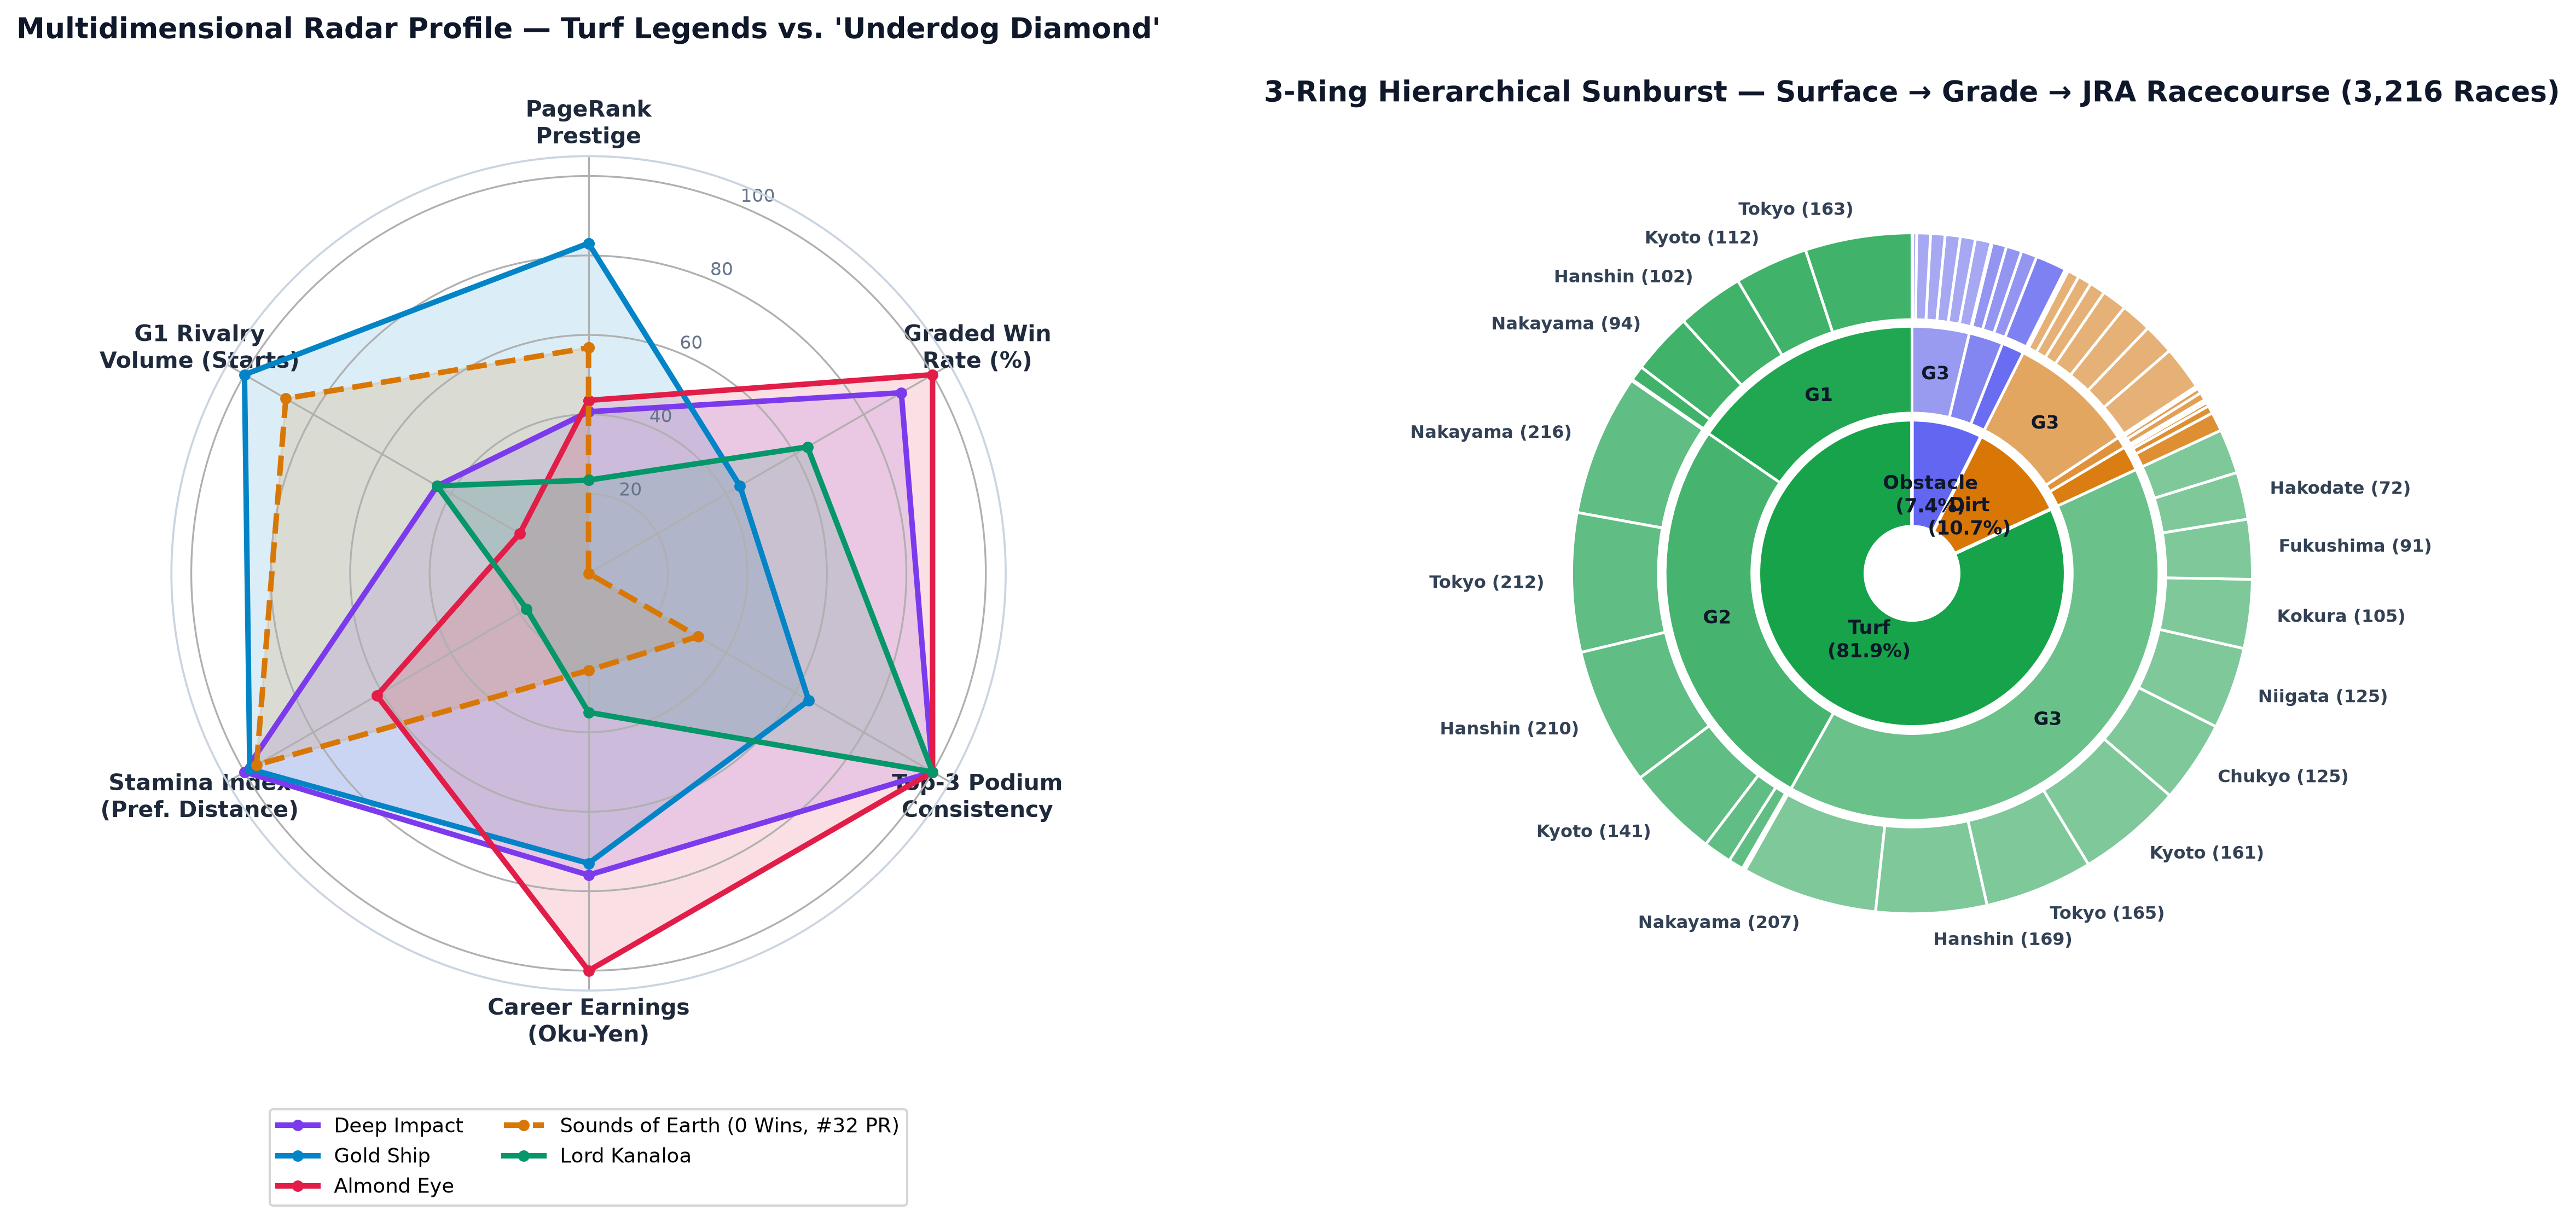
\includegraphics[width=0.95\textwidth]{../assets/superset_radar_and_sunburst.png}}
\caption{Esquerda: Perfil Radar Hexagonal contrastando campeões de G1 com o ``Diamante Injustiçado'' \textit{Sounds of Earth} (\#32 no PageRank com 0 vitórias Graded). Direita: Sunburst Hierárquico de 3 Anéis (\textit{Superfície $\to$ Grau $\to$ 10 Hipódromos da JRA}) sobre as 3.216 corridas.}
\label{fig:radar_sunburst_aeds2}
\end{figure*}

\subsection{Análise Estrutural do DAG de 5 Gerações ($G_p$), LCA e Coeficiente de Endogamia de Wright ($F_X$)}
A avaliação dos algoritmos de travessia em árvore sobre os $|V_p| = 35.149$ nós do DAG genealógico $G_p$ revelou que \textbf{$6.213$ dos $8.202$ cavalos mapeados ($75,75\%$ da população de elite da JRA)} possuem endogamia estritamente positiva dentro do horizonte de 5 gerações ($F_X > 0$), com coeficiente médio populacional de $\bar{F}_X = 0,744\%$ e máximo de $F_X = 8,01\%$.

A aplicação sistemática do algoritmo de Menor Ancestral Comum (LCA) e de filtragem de pares minimais de Wright identificou os grandes patriarcas e matriarcas fundadores sob os quais toda a árvore genealógica do turfe japonês moderno converge em funil (Tabela~IV):
\begin{itemize}
    \item \textbf{\textit{Northern Dancer (CAN)}:} Consagra-se como o ancestral comum mais influente da história do DAG de 5 gerações, aparecendo duplicado simultaneamente nos lados paterno e materno (\textit{inbreeding LCA}) de \textbf{$4.206$ cavalos distintos ($51,28\%$ de toda a base)}, cujos descendentes endogâmicos acumularam \textbf{$1.211$ vitórias em corridas Graded}. Exemplos emblemáticos calculados pelo nosso módulo \path{wright_inbreeding_coefficient} incluem \textbf{\textit{Meisho Samson}} ($F_X = 1,562\%$, com cruzamento $3 \times 4$ em \textit{Northern Dancer}), \textbf{\textit{Tosen Jordan}} ($F_X = 1,758\%$, com cruzamento $4 \times 3$ em \textit{Northern Dancer} e $5 \times 5$ em \textit{Hyperion}), \textbf{\textit{Orfevre}} ($F_X = 1,562\%$, com cruzamento $4 \times 3$ em \textit{Northern Taste}, filho direto de \textit{Northern Dancer}) e \textbf{\textit{Almond Eye}} ($F_X = 1,562\%$, com cruzamento $3 \times 4$ em \textit{Nasrullah}).
    \item \textbf{\textit{Hail to Reason (USA)}, \textit{Almahmoud (USA)} e \textit{Halo (USA)}:} \textit{Hail to Reason} figura como LCA em \textbf{$891$ cavalos endogâmicos} ($256$ vitórias Graded), seguido por \textit{Nasrullah (GB)} ($631$ cavalos e $159$ vitórias) e \textit{Mr. Prospector (USA)} ($409$ cavalos e $69$ vitórias). Destacam-se ainda pela altíssima eficiência competitiva por indivíduo endogâmico a matriarca fundadora \textbf{\textit{Almahmoud (USA)}} ($360$ cavalos endogâmicos e $144$ vitórias Graded, liderando a eficiência da tabela com \textbf{$0,400$ vitórias Graded por indivíduo}) e seu neto \textbf{\textit{Halo (USA)}} (pai de \textit{Sunday Silence}, com $268$ cavalos endogâmicos, $100$ vitórias Graded e \textbf{$0,373$ vitórias por animal}, presente em cruzamentos múltiplos como os de \textit{Cheval Grand} e \textit{Satono Diamond}, ambos com $F_X = 2,734\%$).
\end{itemize}

\begin{table}[htbp]
\caption{Principais Ancestrais Fundadores (LCA) no DAG de 5 Gerações ($G_p$) Ordenados por Alcance de Endogamia ($F_X > 0$)}
\begin{center}
\renewcommand{\arraystretch}{1.15}
\setlength{\tabcolsep}{4.0pt}
\resizebox{\columnwidth}{!}{%
\begin{tabular}{clccc}
\toprule
\textbf{Rank DAG} & \textbf{Ancestral Comum (LCA em $G_p$)} & \textbf{Cavalos c/ Inbreeding} & \textbf{Vitórias Graded} & \textbf{Vit. / Cavalo} \\
\midrule
\#1 & \textbf{Northern Dancer (CAN)} & $\mathbf{4.206}$ & $\mathbf{1.211}$ & $0,288$ \\
\#2 & \textbf{Hail to Reason (USA)} & $891$ & $256$ & $0,287$ \\
\#3 & \textbf{Nasrullah (GB)} & $631$ & $159$ & $0,252$ \\
\#4 & \textbf{Mr. Prospector (USA)} & $409$ & $69$ & $0,169$ \\
\#5 & \textbf{Native Dancer (USA)} & $384$ & $74$ & $0,193$ \\
\#6 & \textbf{Almahmoud (USA)} & $\mathbf{360}$ & $\mathbf{144}$ & $\mathbf{0,400}$ \\
\#7 & \textbf{Raise a Native (USA)} & $352$ & $64$ & $0,182$ \\
\#8 & \textbf{Halo (USA)} & $\mathbf{268}$ & $\mathbf{100}$ & $\mathbf{0,373}$ \\
\#9 & \textbf{Nearco (ITY)} & $244$ & $43$ & $0,176$ \\
\#10 & \textbf{Nearctic (CAN)} & $205$ & $49$ & $0,239$ \\
\bottomrule
\end{tabular}%
}
\label{tab:inbreeding_lca_aeds2}
\end{center}
\end{table}

Na geração imediata (nível $l = 1$ da árvore, Fig.~4), verifica-se a hegemonia reprodutiva de \textbf{\textit{Deep Impact}} (289 filhos únicos em provas Graded, 1.541 largadas e 46 títulos de G1) e de seu pai \textbf{\textit{Sunday Silence (USA)}} (281 filhos únicos, 1.793 largadas e 42 títulos de G1), seguidos por \textbf{\textit{King Kamehameha}} (212 filhos), \textbf{\textit{Fuji Kiseki}} (173) e \textbf{\textit{Stay Gold}} (133), ao passo que \textbf{\textit{Almond Eye}} (¥19,15 Bilhões / $1.915,3\text{ milhões de ienes}$) e \textbf{\textit{Kitasan Black}} (¥18,77 Bilhões) lideram o ranking de premiação acumulada nos vértices de $G_c$.

\begin{figure}[htbp]
\centerline{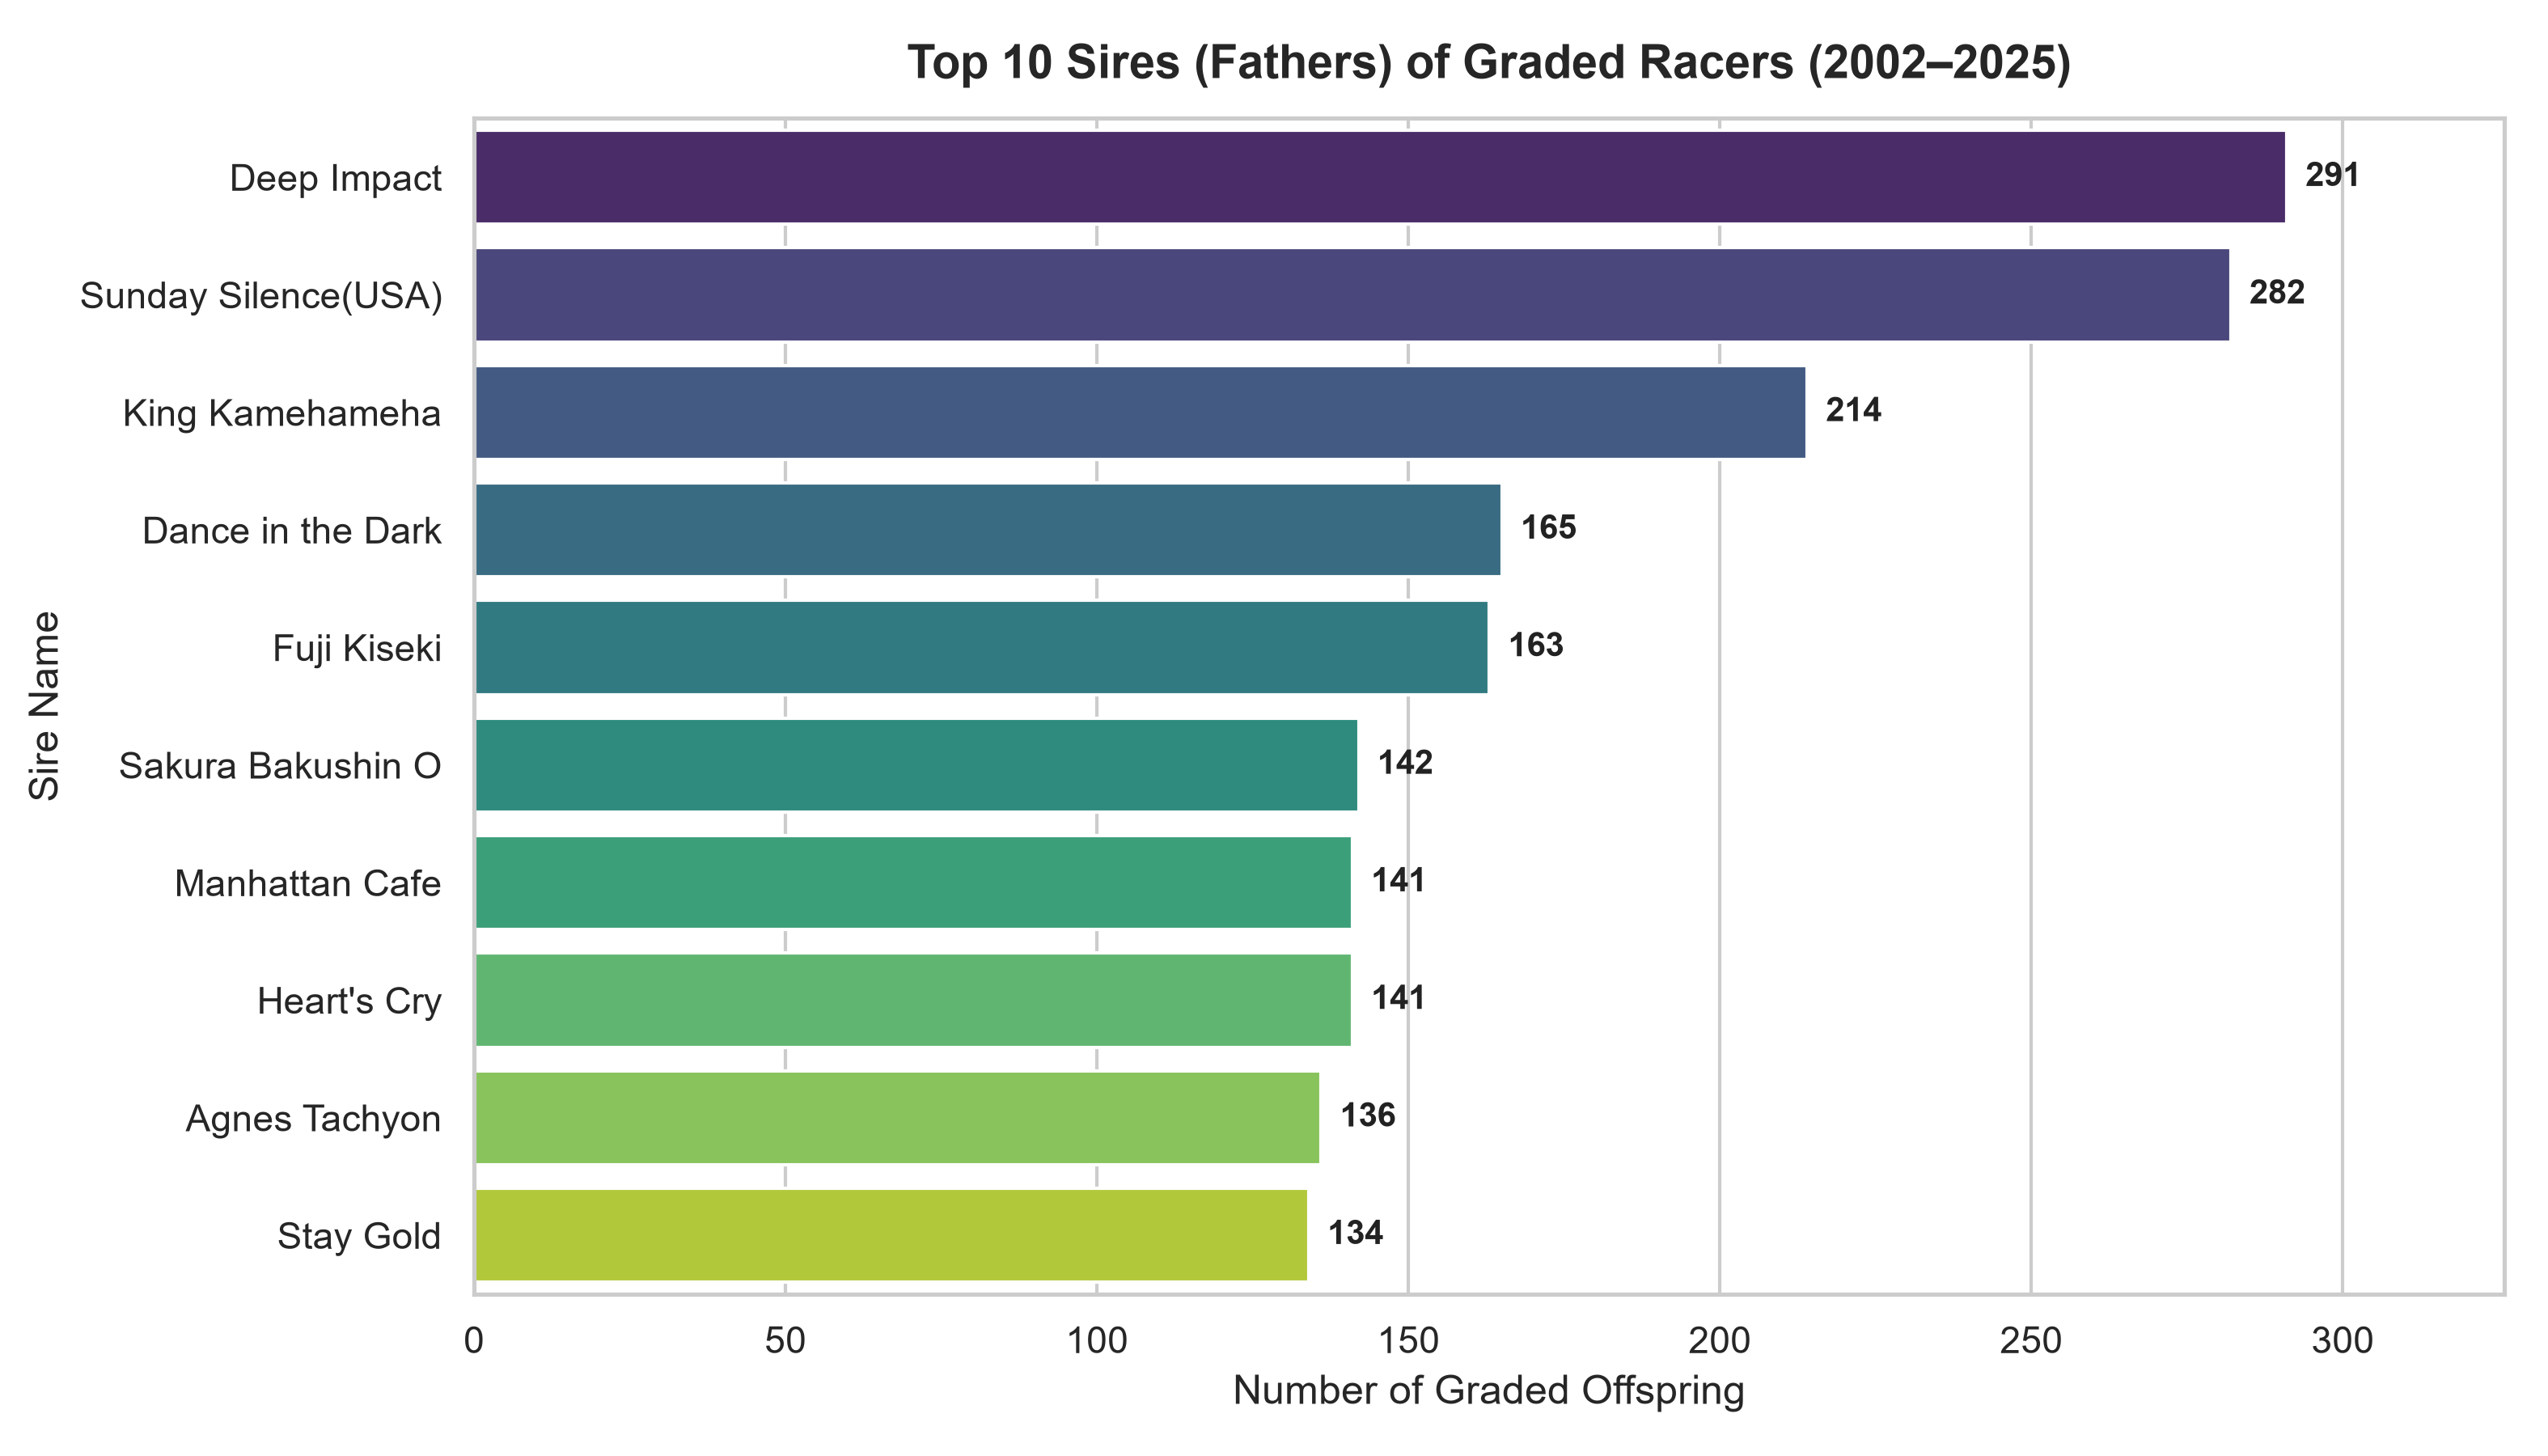
\includegraphics[width=0.98\columnwidth]{../assets/top_sires.png}}
\vspace{2mm}
\centerline{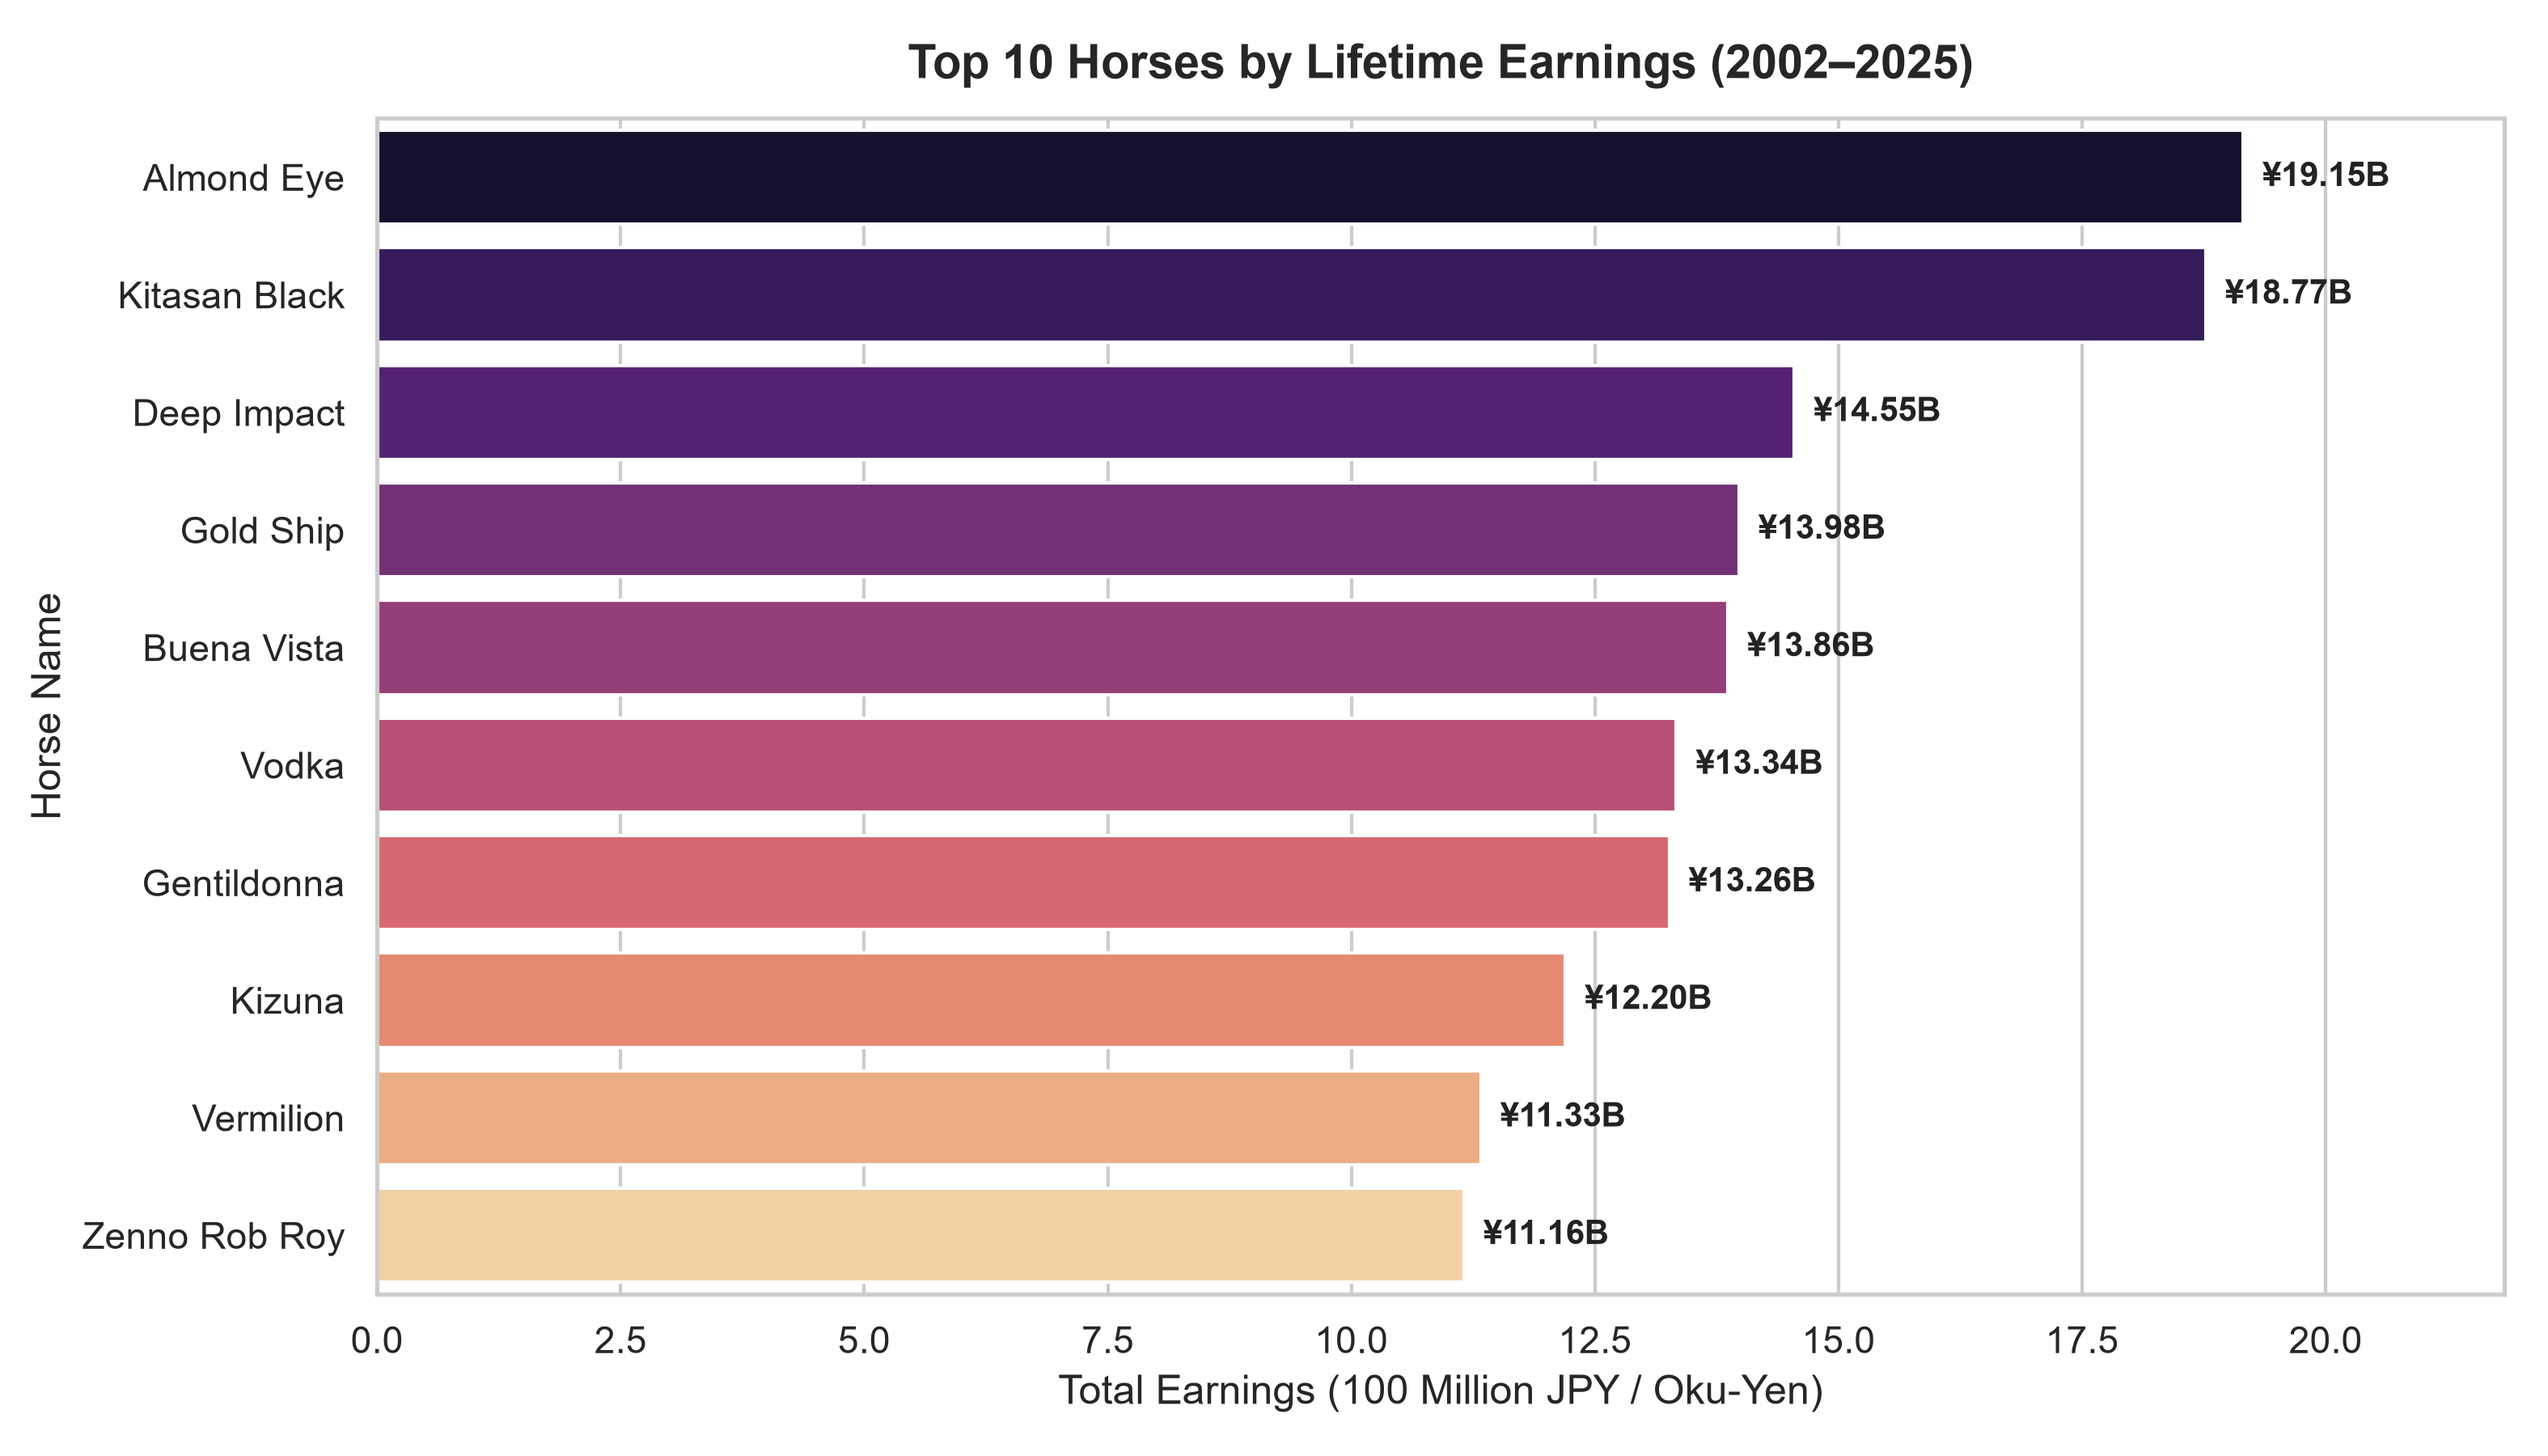
\includegraphics[width=0.98\columnwidth]{../assets/top_earners.png}}
\caption{Acima: Grau de saída reprodutivo no nível $l=1$ do DAG $G_p$ (Top 10 garanhões por prole única em provas Graded). Abaixo: Top 10 vértices de $G_c$ por premiação acumulada na carreira (em 100 milhões de ienes / \textit{Oku-Yen}).}
\label{fig:top_sires_earners_aeds2}
\end{figure}

Para visualizar a propagação de fluxo ao longo das ramificações do DAG até as pistas, o \textbf{Diagrama de Fluxo Aluvial / Sankey de 4 Estágios} (Fig.~5) mapeia $N = 8.857$ participações através das partições \textit{Linhagem Paterna} $\to$ \textit{Superfície} $\to$ \textit{Regime de Distância} $\to$ \textit{Grau (G1/G2/G3)}. Observa-se nitidamente a bifurcação topológica das linhagens: enquanto os ramos de \textit{Deep Impact}, \textit{Sunday Silence} e \textit{King Kamehameha} fluem para a Grama (\textit{Turf}, $92,6\%$) e distâncias clássicas ($1800\text{--}2200\text{m}$, $45,6\%$), os ramos laranjas de \textbf{\textit{Gold Allure}} e \textbf{\textit{Brian's Time}} desviam fortemente para a Areia (\textit{Dirt}), e o ramo azul-claro de \textbf{\textit{Sakura Bakushin O}} canaliza-se para o regime de velocidade curta (\textit{Sprint} $\le 1400\text{m}$). Complementarmente, o \textbf{Streamgraph Simétrico Temporal} (Fig.~6) demonstra a dinâmica de sucessão geracional das árvores ao longo do tempo em três ondas: a Era I (2002--2007) dominada por \textit{Sunday Silence} e \textit{Brian's Time}; a Era II (2008--2012) marcada por \textit{Fuji Kiseki}, \textit{Agnes Tachyon}, \textit{Dance in the Dark} e \textit{Manhattan Cafe}; e a Era III (2013+) dominada por \textit{Deep Impact}, \textit{King Kamehameha}, \textit{Stay Gold}, \textit{Heart's Cry} e \textit{Lord Kanaloa}.

\begin{figure*}[htbp]
\centerline{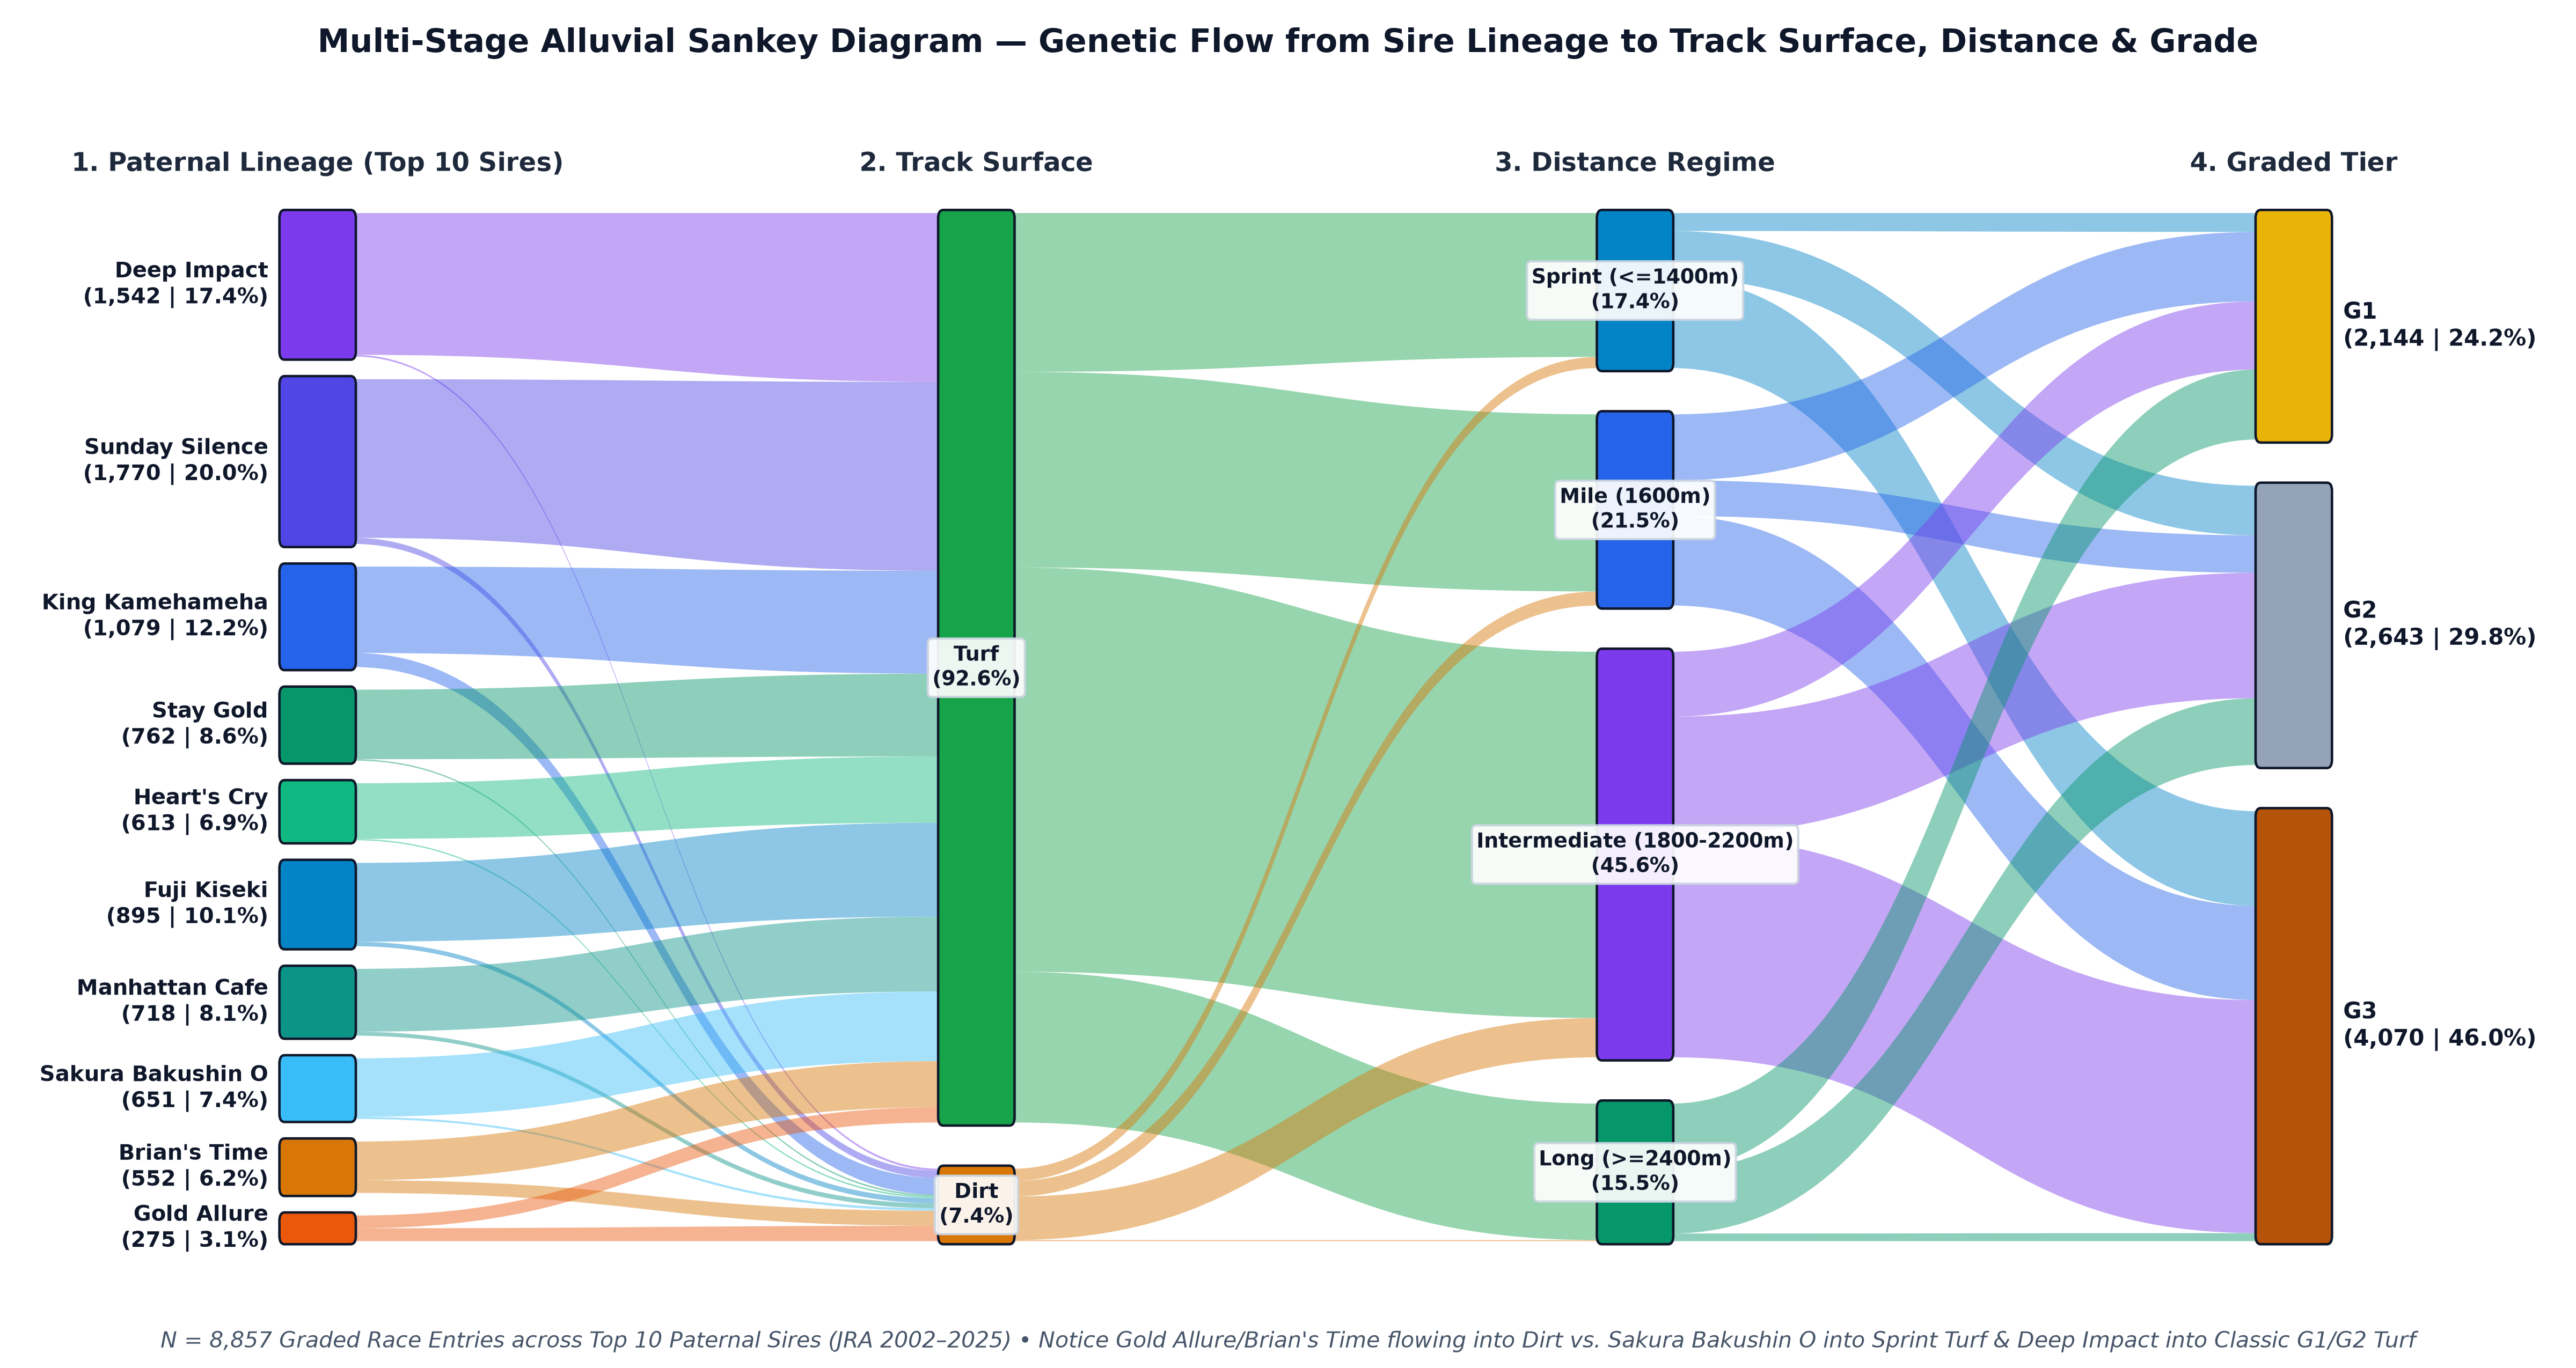
\includegraphics[width=0.95\textwidth]{../assets/superset_alluvial_sankey_flow.png}}
\caption{Diagrama de Fluxo Aluvial / Sankey de 4 Estágios: propagação de fluxo das 10 maiores subárvores paternas do DAG para Superfície, Regime de Distância e Grau da Corrida ($N = 8.857$ participações).}
\label{fig:sankey_aeds2}
\end{figure*}

\begin{figure*}[htbp]
\centerline{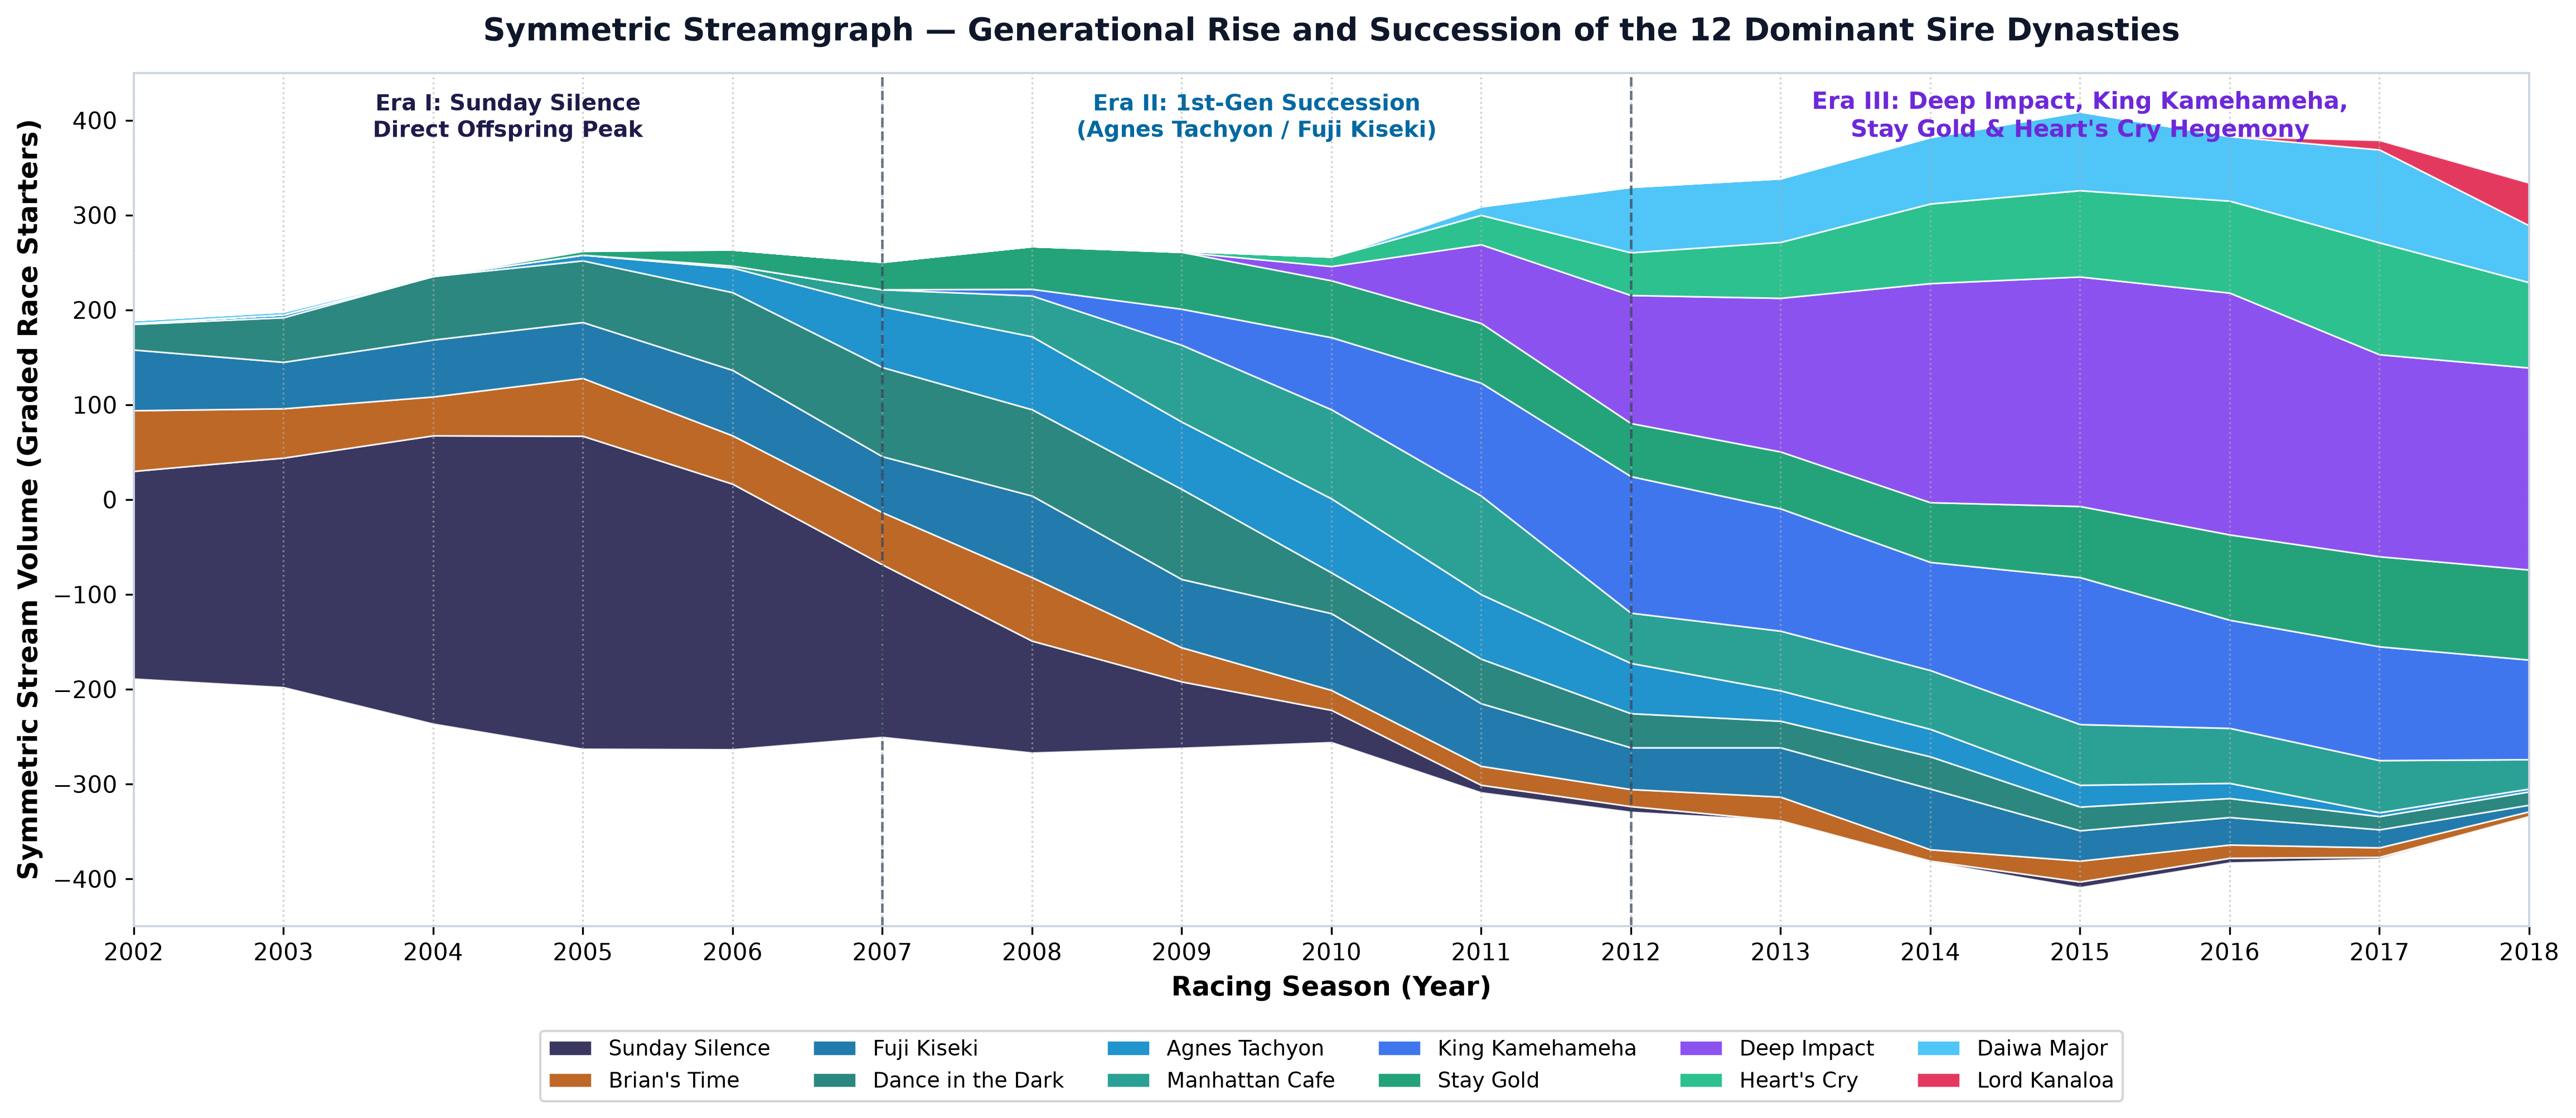
\includegraphics[width=0.92\textwidth]{../assets/superset_streamgraph_dynasties.png}}
\caption{Streamgraph Simétrico Temporal ilustrando a substituição geracional entre as 12 principais dinastias paternas do DAG $G_p$ ao longo das temporadas.}
\label{fig:streamgraph_aeds2}
\end{figure*}

\subsection{Visualização Topológica Vetorial no Gephi (ForceAtlas2) e Grafos Bipartidos}
A espacialização contínua via algoritmo \textbf{ForceAtlas2} no software \textbf{Gephi} [10, 11] (Fig.~7) permitiu inspecionar a estrutura mesoscópica dos quatro grafos construídos (\path{data/gephi/}):
\begin{enumerate}
    \item \textbf{Rede de Competição Top 150 PageRank (Fig.~7, esquerda, $150$ vértices e $2.551$ arestas):} A coloração por clã paterno e o dimensionamento proporcional ao PageRank demonstram que os filhos de \textit{Deep Impact} (azul) e \textit{Sunday Silence} (roxo) ocupam o núcleo densamente interconectado de Grau 1, enquanto especialistas de milha e areia orbitam em comunidades periféricas de alta modularidade.
    \item \textbf{Galáxia Genealógica de 5 Gerações no DAG $G_p$ (Fig.~7, direita, $4.475$ vértices de elite e $6.042$ arestas):} O layout de repulsão-atração revela visualmente o efeito funil do colapso de pedigree: milhares de folhas contemporâneas convergem radialmente sobre dois super-atratores gravitacionais no centro do grafo, representados por \textbf{\textit{Sunday Silence (USA)}} e \textbf{\textit{Northern Dancer (CAN)}}.
    \item \textbf{Grafos Bipartidos Jóquei--Cavalo ($G_{jc}$) e Jóquei--Treinador ($G_{jt}$):} A análise dos pesos das arestas em $G_{jc}$ destacou as maiores parcerias ponderadas por Grau da história moderna: \textbf{Yutaka Take $\leftrightarrow$ Deep Impact}, \textbf{Christophe Lemaire $\leftrightarrow$ Almond Eye}, \textbf{Yutaka Take $\leftrightarrow$ Kitasan Black}, \textbf{Kenichi Ikezoe $\leftrightarrow$ Orfevre} e \textbf{Mirco Demuro $\leftrightarrow$ Duramente}. No grafo $G_{jt}$, a maior aresta de colaboração profissional une o jóquei \textbf{Yutaka Take} e os grandes treinadores de Ritto (\textit{Yasuo Tomomichi}, \textit{Katsuhiko Sumii} e \textit{Yasutoshi Ikee}).
\end{enumerate}

\begin{figure}[htbp]
\centerline{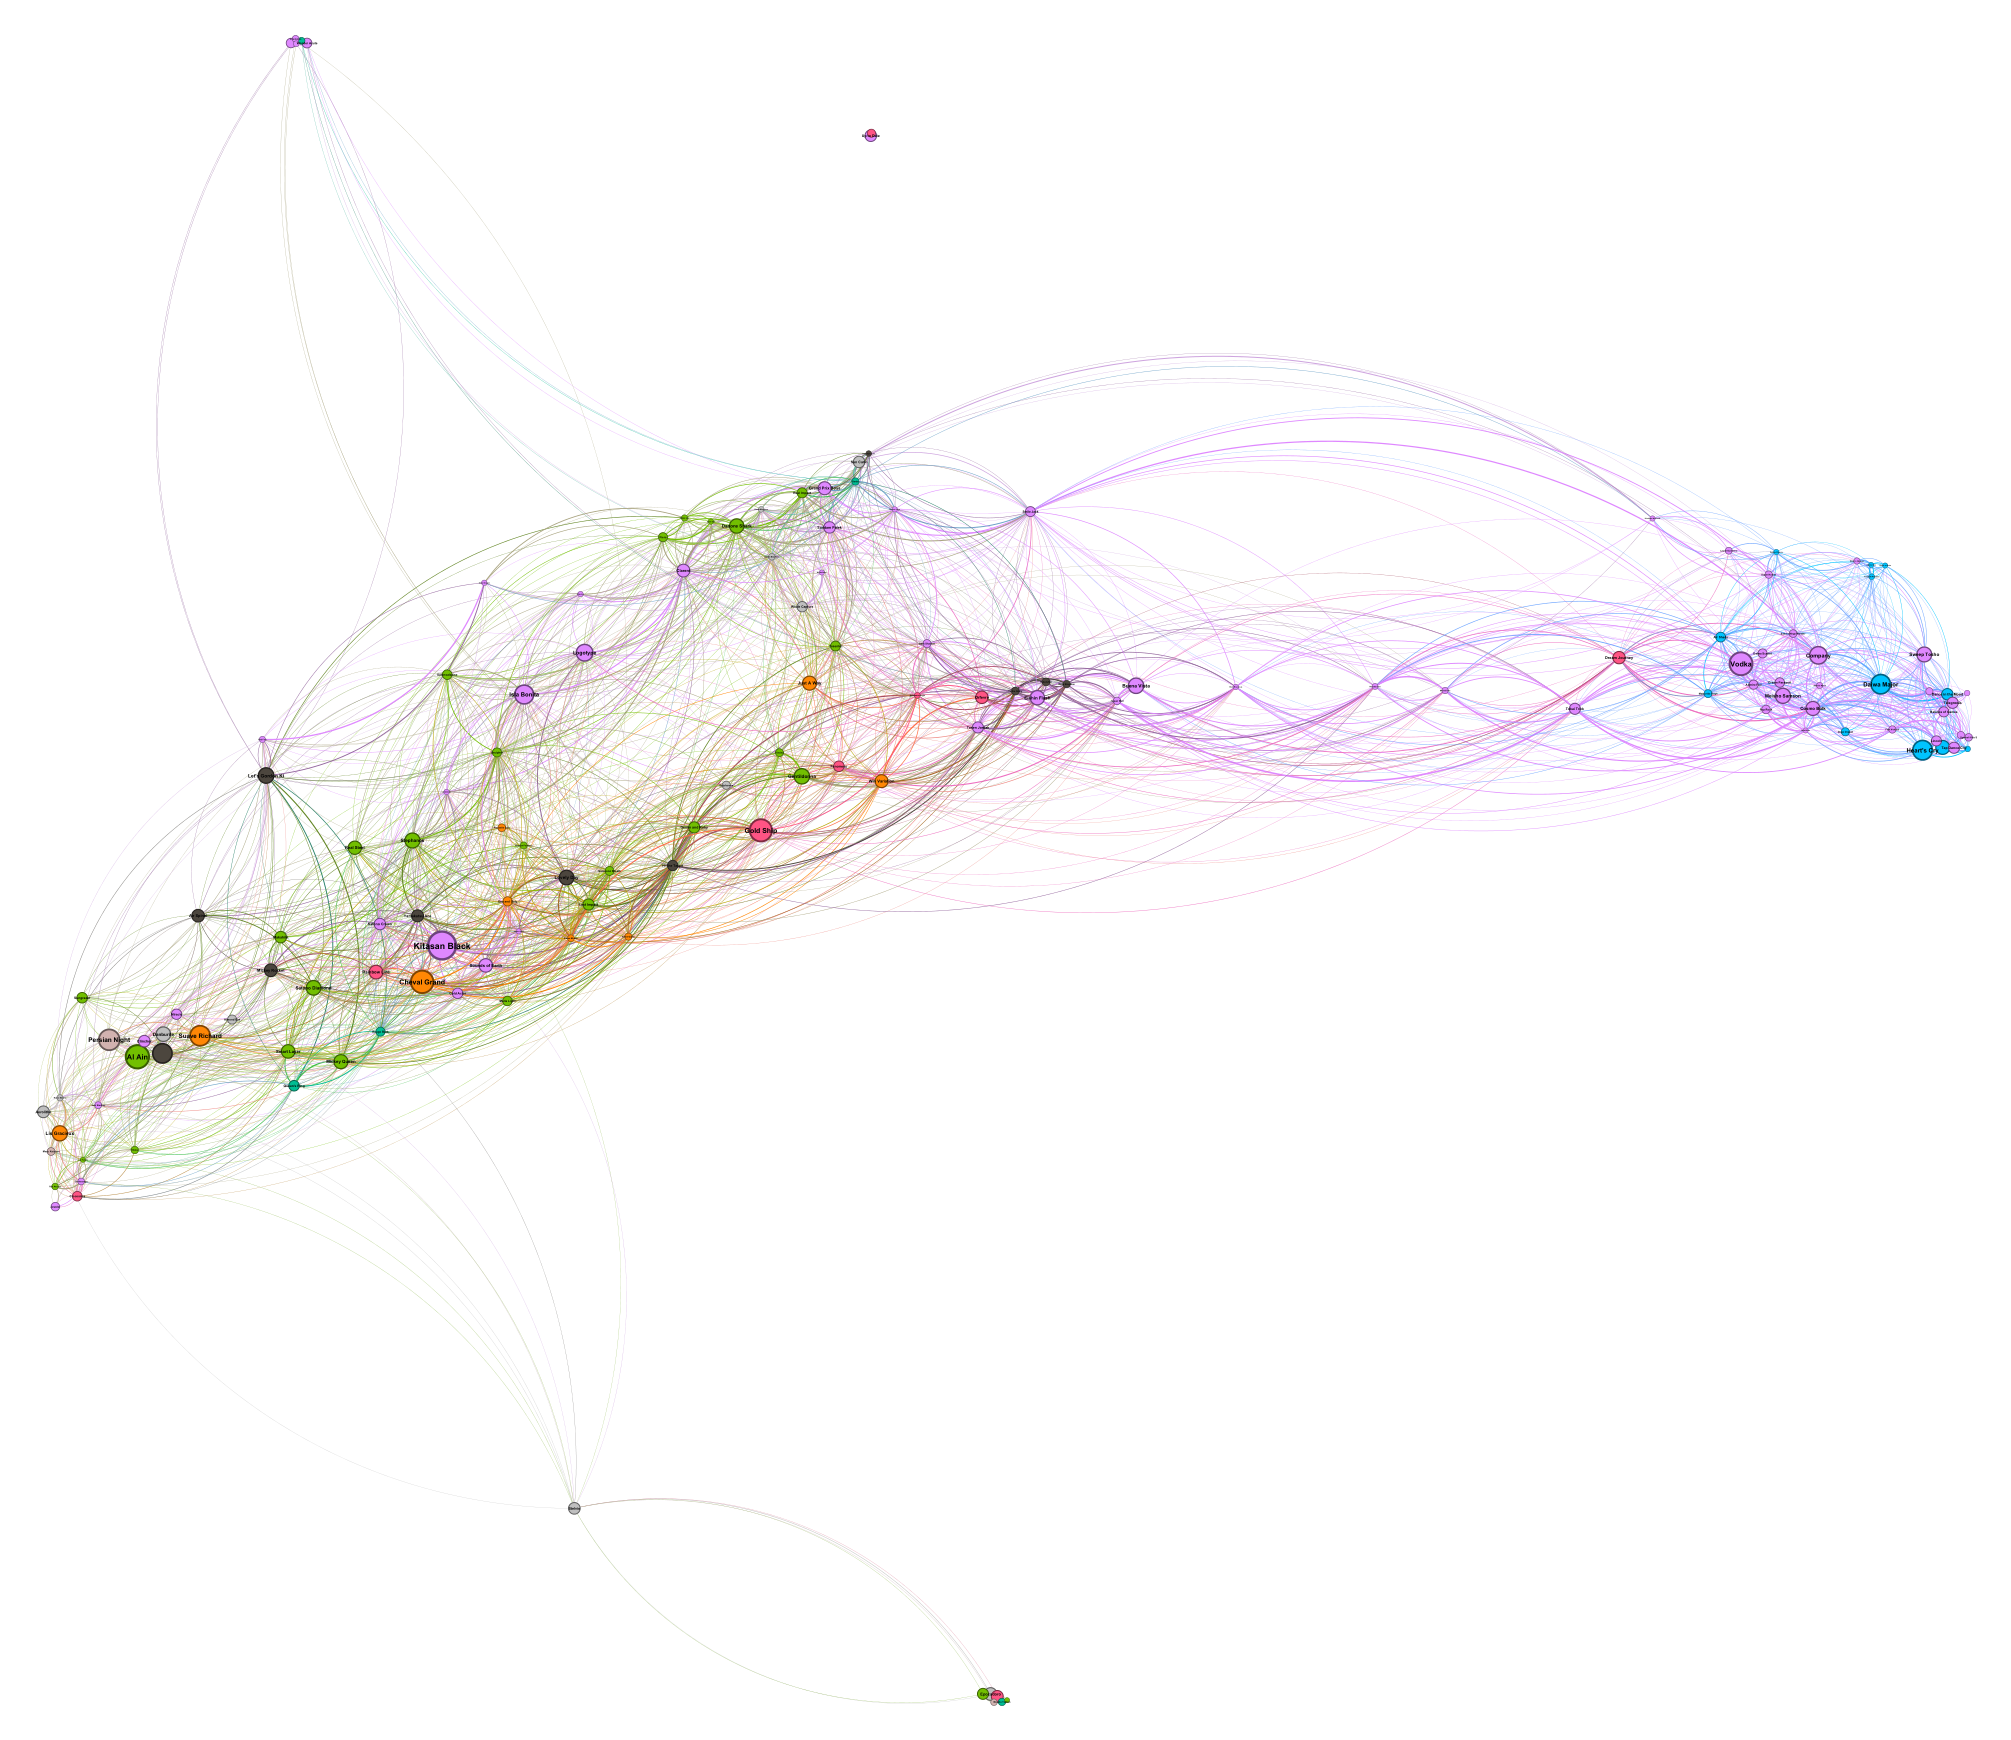
\includegraphics[width=0.49\columnwidth]{../assets/gephi_competition_top150.png}\hfill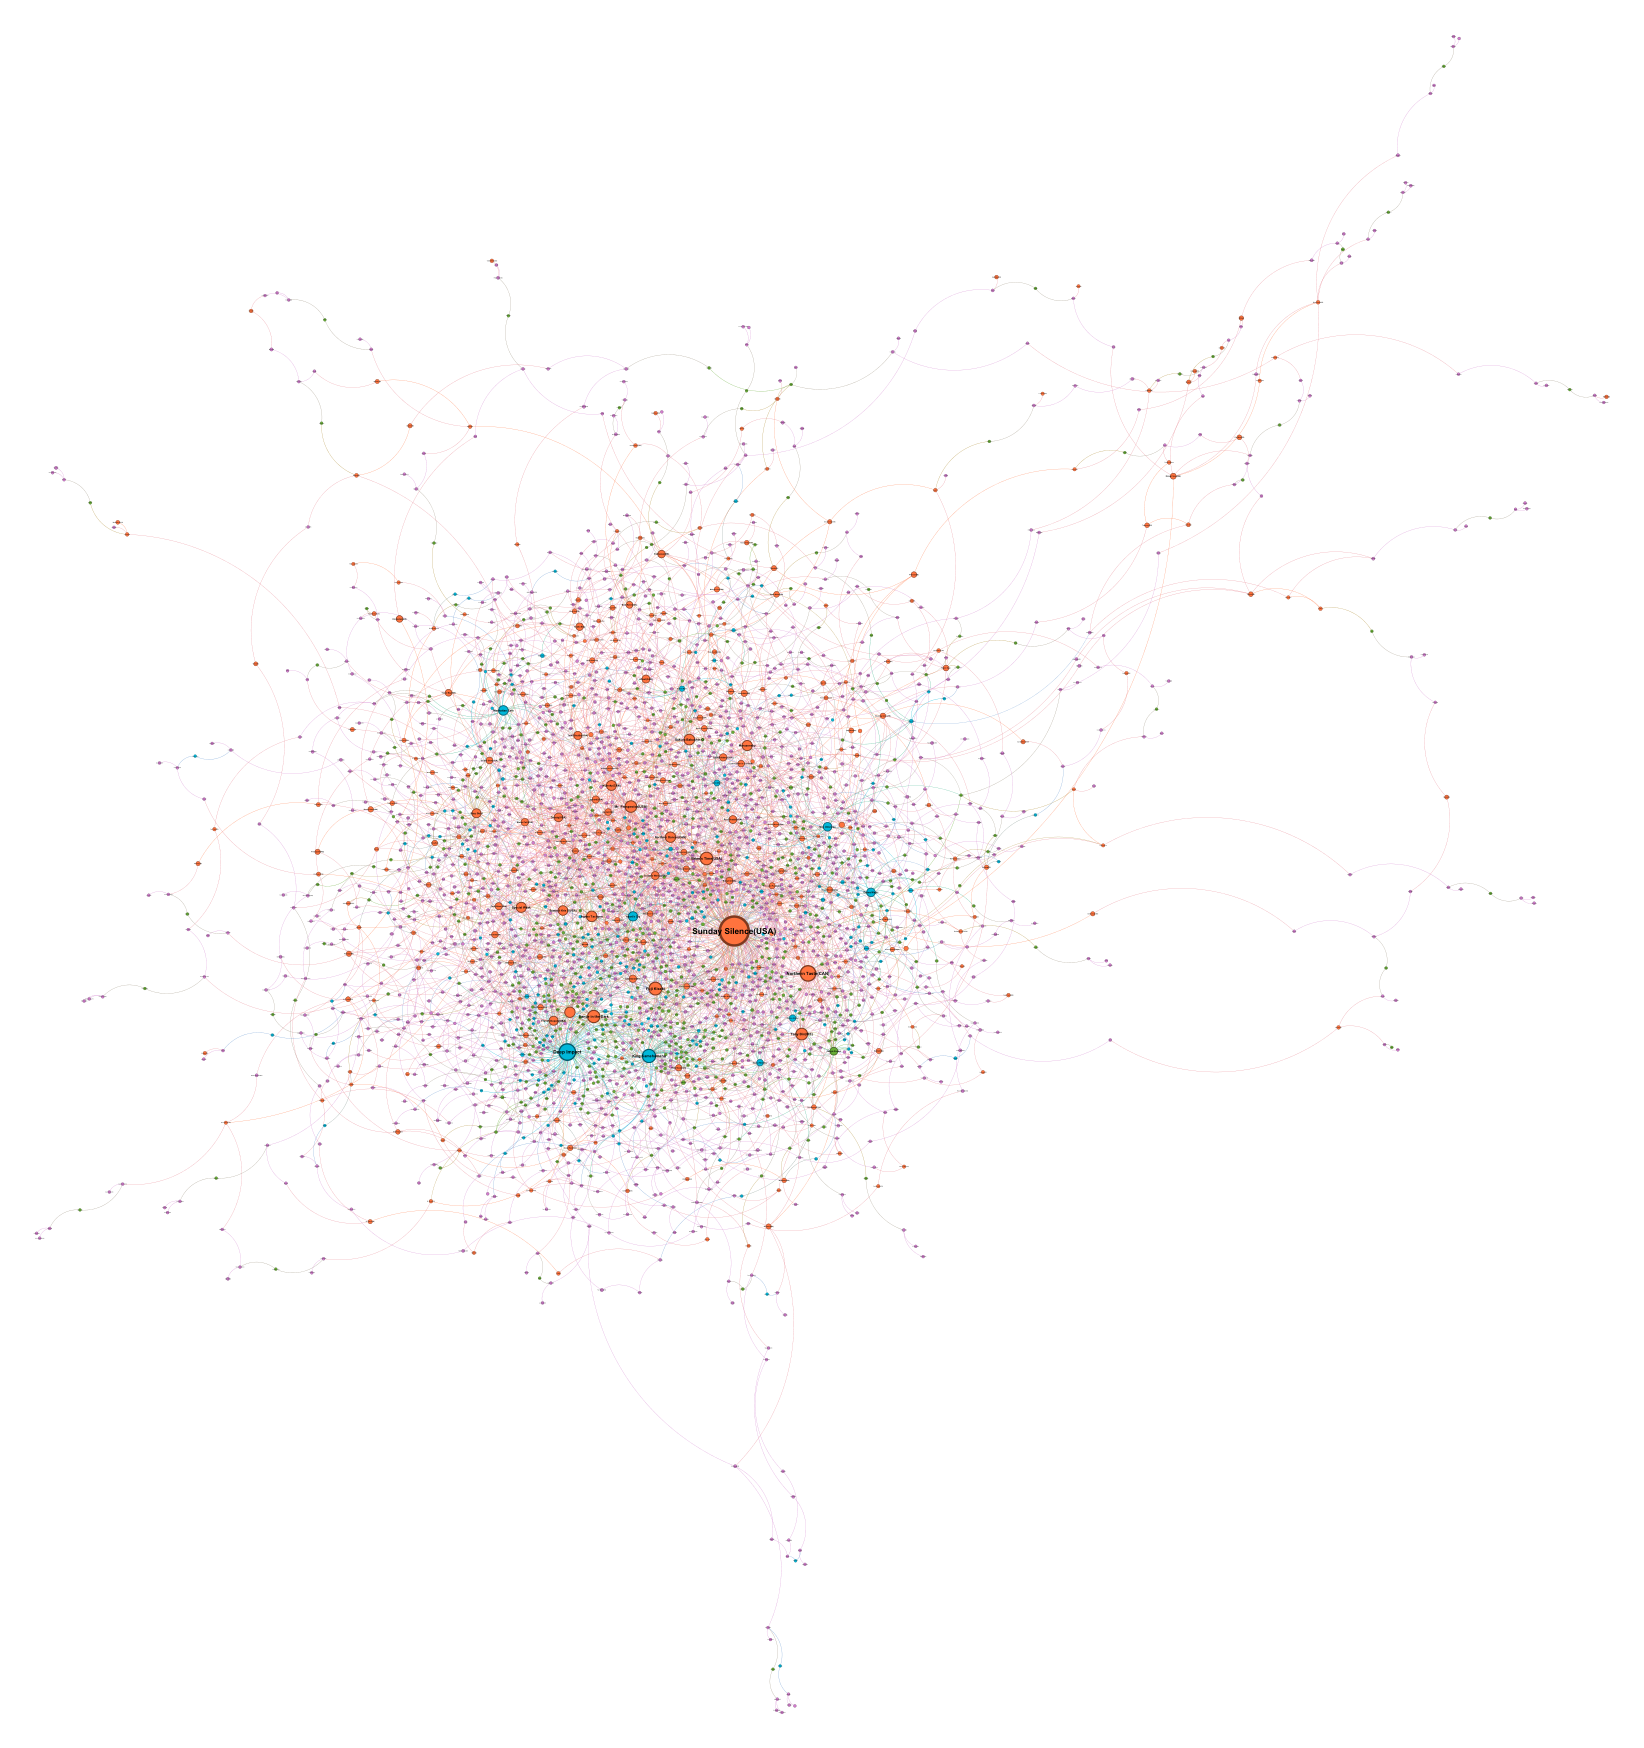
\includegraphics[width=0.49\columnwidth]{../assets/gephi_lineage_dag_elite.png}}
\caption{Visualizações vetoriais geradas no Gephi via algoritmo ForceAtlas2 [10, 11]. Esquerda: Subgrafo de Competição Top 150 PageRank ($2.551$ arestas). Direita: Subgrafo de Elite do DAG Genealógico de 5 Gerações ($4.475$ vértices e $6.042$ arestas) evidenciando os super-hubs \textit{Sunday Silence} e \textit{Northern Dancer}.}
\label{fig:gephi_networks_aeds2}
\end{figure}

\subsection{Especialização Genética, Biometria, K-Means++ PCA e Random Forest Out-of-Time}
Cruzando a topologia do DAG $G_p$ com os atributos físicos das corridas, o teste Qui-Quadrado de independência rejeitou a hipótese nula de neutralidade genética com significância extrema tanto para a superfície da pista ($\chi^2 = 739,99, gl = 14, p = 2,43 \times 10^{-107}, V \text{ de Cramér} = 0,2514$) quanto para o regime de distância ($\chi^2 = 2237,47, gl = 42, p = 3,71 \times 10^{-317}, V = 0,2523$; ANOVA One-Way $F(14, 930) = 16,46, \eta^2 = 0,1986, p = 1,68 \times 10^{-35}$; Kruskal-Wallis $H = 192,40, p = 2,02 \times 10^{-29}$). Adicionalmente, o gráfico \textbf{Split-Violin} da massa corporal no dia da prova (Fig.~8, esquerda) comprovou um dimorfismo biomecânico consistente em todas as distâncias: competidores de \textbf{Areia (\textit{Dirt}, média $494,0\text{ a }498,2\text{ kg}$)} são de \textbf{$16\text{ kg a }21\text{ kg}$ mais pesados} que os competidores de \textbf{Grama (\textit{Turf}, média $473,0\text{ a }482,4\text{ kg}$)}.

\begin{figure*}[htbp]
\centerline{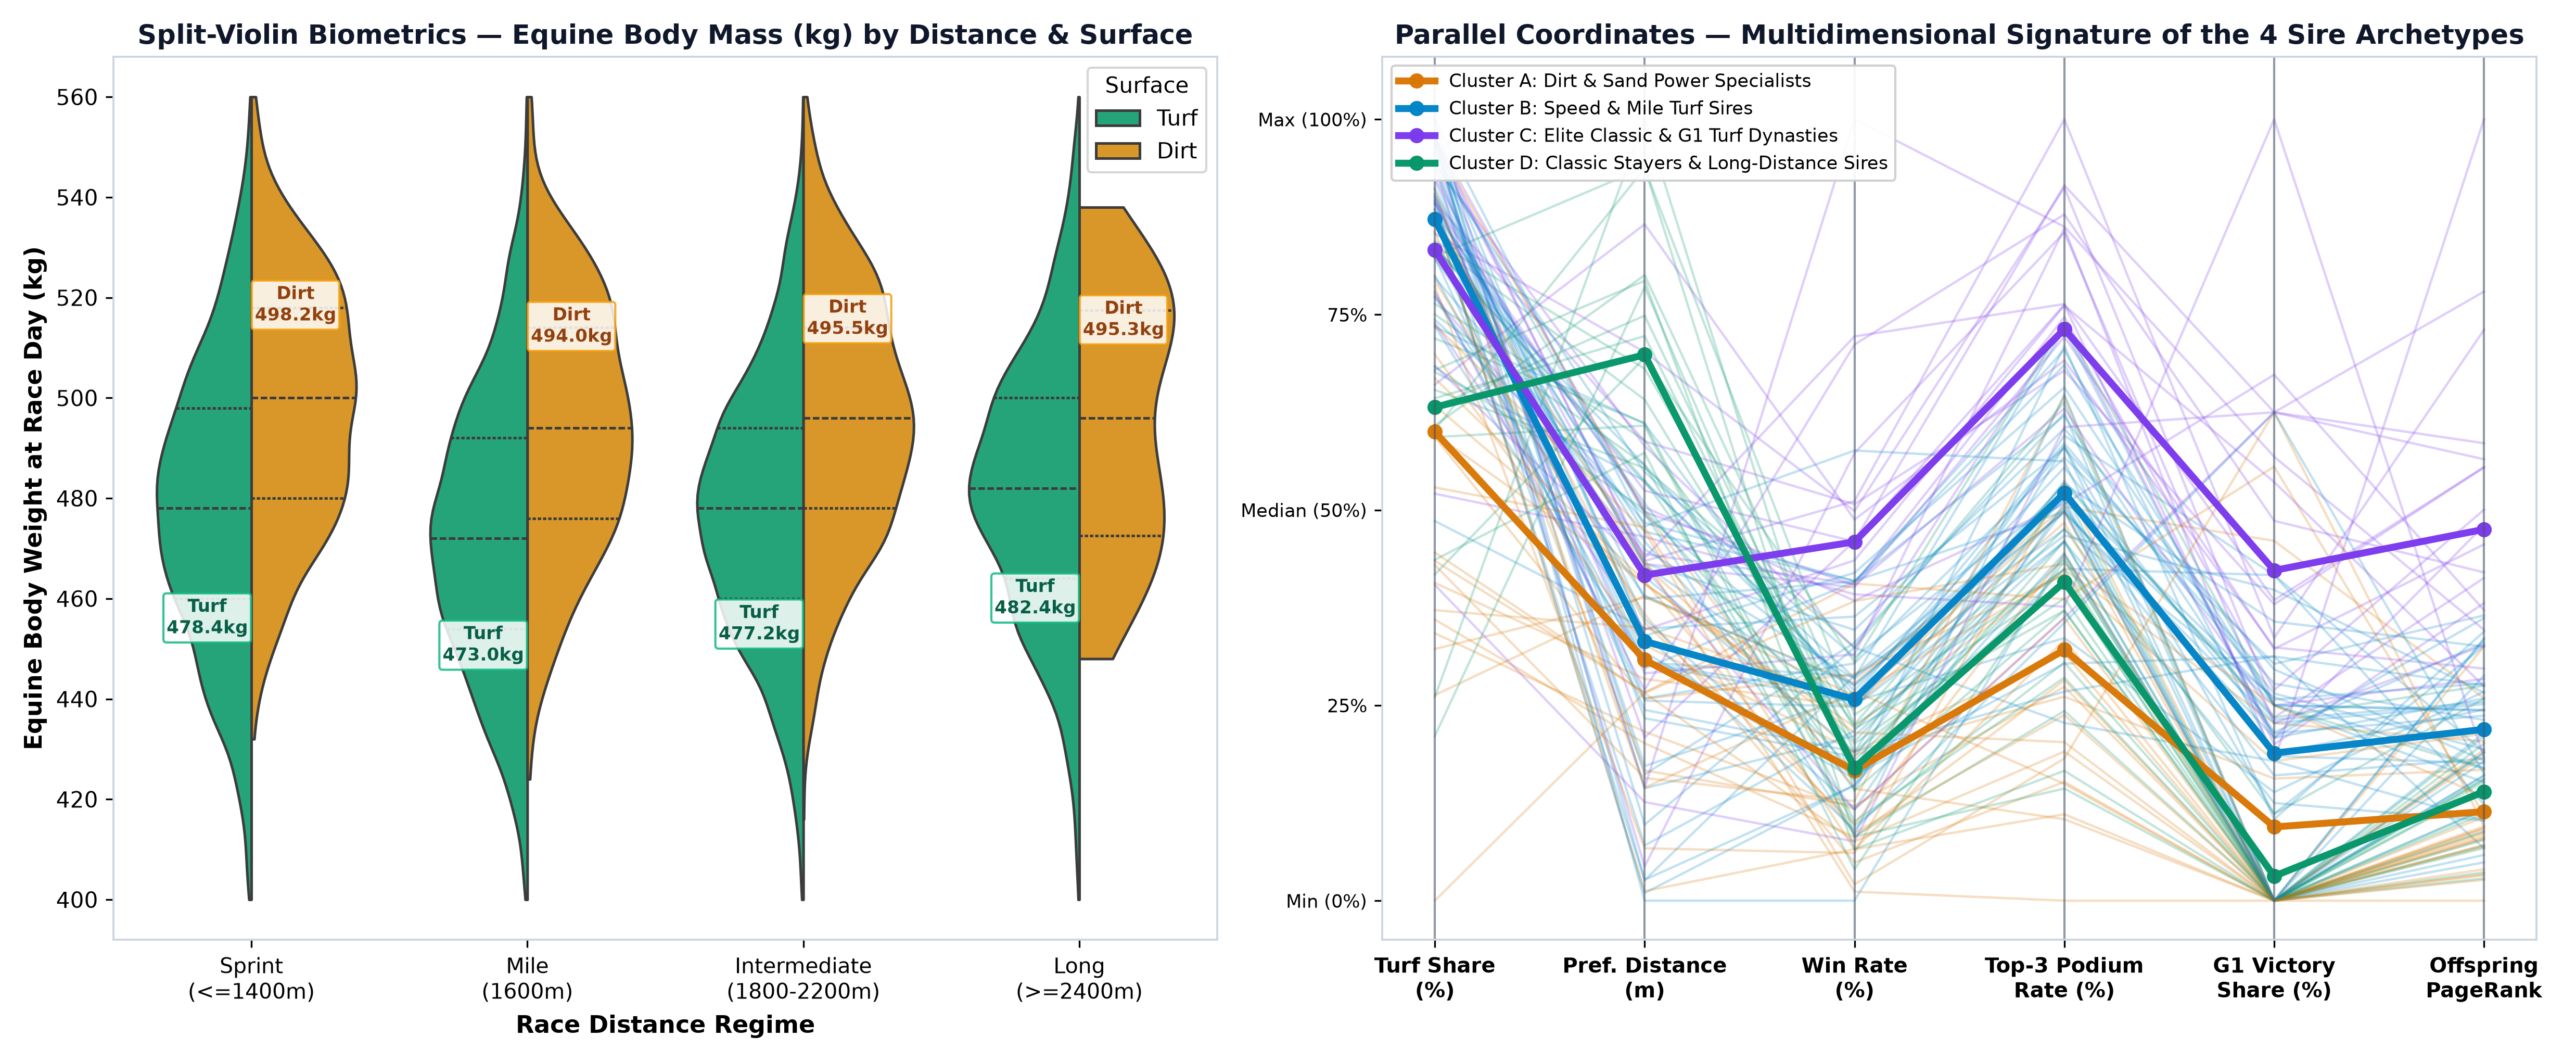
\includegraphics[width=0.95\textwidth]{../assets/superset_raincloud_and_parallel.png}}
\caption{Esquerda: Distribuição Split-Violin da massa corporal equina (kg) por regime de distância e superfície (\textit{Turf} vs. \textit{Dirt}). Direita: Coordenadas Paralelas traçando a assinatura multidimensional dos 106 principais garanhões nos 6 indicadores topológicos e zootécnicos.}
\label{fig:violin_parallel_aeds2}
\end{figure*}

Na modelagem não-supervisionada dos 106 principais garanhões (Fig.~9), os dois primeiros eixos da Análise de Componentes Principais capturaram \textbf{$63,4\%$ da variância total} ($\text{PC}_1 = 44,1\%$ e $\text{PC}_2 = 19,2\%$), e o algoritmo \textbf{K-Means++} [12] segmentou os vértices paternos em quatro arquétipos zootécnicos: \textbf{Cluster A} (\textit{Dirt \& Sand Power Specialists}, $n = 26$: \textit{Gold Allure}, \textit{Brian's Time}), \textbf{Cluster B} (\textit{Speed \& Mile Turf Sires}, $n = 41$: \textit{Sakura Bakushin O}, \textit{Fuji Kiseki}), \textbf{Cluster C} (\textit{Elite Classic \& G1 Turf Dynasties}, $n = 20$: \textit{Deep Impact}, \textit{Sunday Silence}, \textit{King Kamehameha}, \textit{Stay Gold}) e \textbf{Cluster D} (\textit{Classic Stayers \& Long-Distance Sires}, $n = 19$: \textit{Dance in the Dark}, \textit{Mayano Top Gun}).

\begin{figure*}[htbp]
\centerline{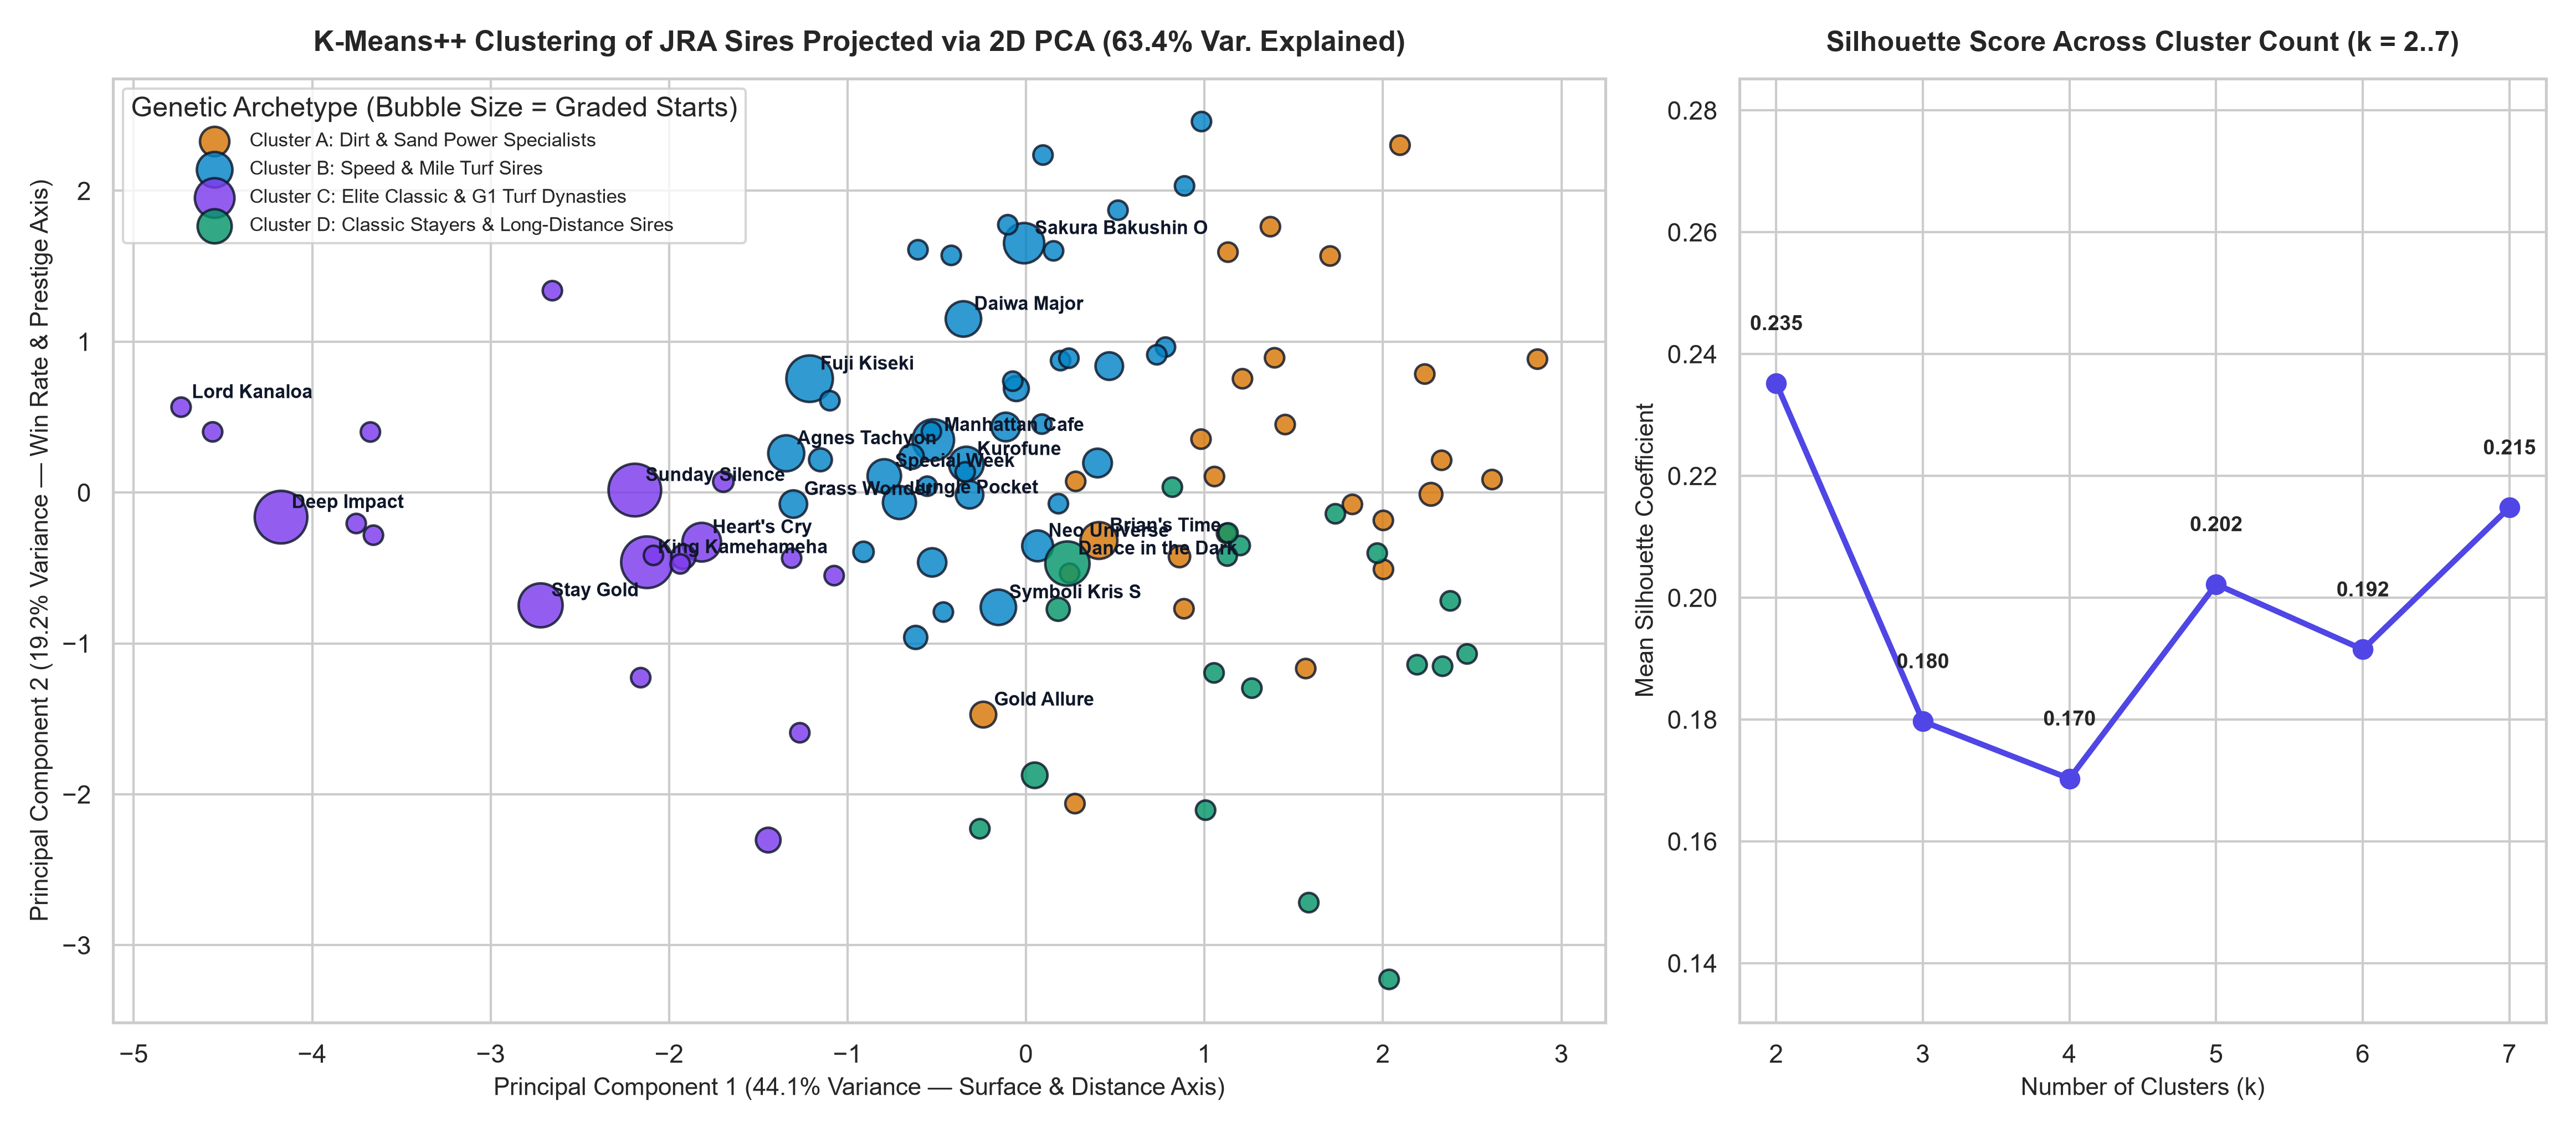
\includegraphics[width=0.94\textwidth]{../assets/ml_kmeans_pca_clusters.png}}
\caption{Esquerda: Agrupamento K-Means++ [12] dos 106 garanhões projetado via PCA 2D ($63,4\%$ de variância explicada). Direita: Curva de Silhouette Score para $k \in \{2 \dots 7\}$.}
\label{fig:kmeans_pca_aeds2}
\end{figure*}

Por fim, na predição supervisionada de pódio (Top-3) avaliada no conjunto de teste cronológico futuro (\textbf{2016--2018, $N_{\text{teste}} = 5.889$, \textit{Zero Data Leakage}}, Tabela~V e Fig.~10), o classificador \textbf{Random Forest} [13] atingiu \textbf{$\text{ROC-AUC} = 0,7260$} (IC Bootstrap 95\%: $[0,7109;\; 0,7389]$), $\text{PR-AUC} = 0,4187$ e $\text{F1-Score} = 0,4585$, superando a Regressão Logística L2 ($\text{ROC-AUC} = 0,7144$). A decomposição da Importância de Gini (Fig.~10, esquerda) revela que as métricas extraídas da rede bipartida e do histórico temporal lideram o poder preditivo na largada: a \textbf{taxa histórica prévia do jóquei ($29,77\%$)} e o \textbf{retrospecto prévio do próprio cavalo ($22,70\%$)} respondem por mais de $52\%$ da decisão do modelo, seguidos pela idade ($9,09\%$), número de largadas prévias ($5,70\%$), tamanho do grid ($5,10\%$), taxa prévia do treinador ($4,90\%$), peso de grau da corrida ($4,28\%$), afinidade genética do garanhão com a superfície no DAG ($3,88\%$) e retrospecto do avô materno ($2,92\%$).

\begin{table}[htbp]
\caption{Desempenho Preditivo de Pódio (Top-3) no Conjunto de Teste Cronológico Out-of-Time (2016--2018, $N = 5.889$)}
\begin{center}
\renewcommand{\arraystretch}{1.15}
\setlength{\tabcolsep}{3.5pt}
\resizebox{\columnwidth}{!}{%
\begin{tabular}{lcccc}
\toprule
\textbf{Modelo Supervisionado} & \textbf{ROC-AUC (IC 95\%)} & \textbf{PR-AUC} & \textbf{F1} & \textbf{Acc.} \\
\midrule
Baseline Estratificado & $0,5000$ (---) & $0,2089$ & $0,0000$ & $0,7918$ \\
Regressão Logística L2 & $0,7144$ ($[0,699;\; 0,728]$) & $\mathbf{0,4257}$ & $0,4413$ & $0,6762$ \\
\textbf{Random Forest (CART)} & $\mathbf{0,7260}$ ($\mathbf{[0,711;\; 0,739]}$) & $0,4187$ & $\mathbf{0,4585}$ & $\mathbf{0,6908}$ \\
\bottomrule
\end{tabular}%
}
\label{tab:ml_results_aeds2}
\end{center}
\end{table}

\begin{figure*}[htbp]
\centerline{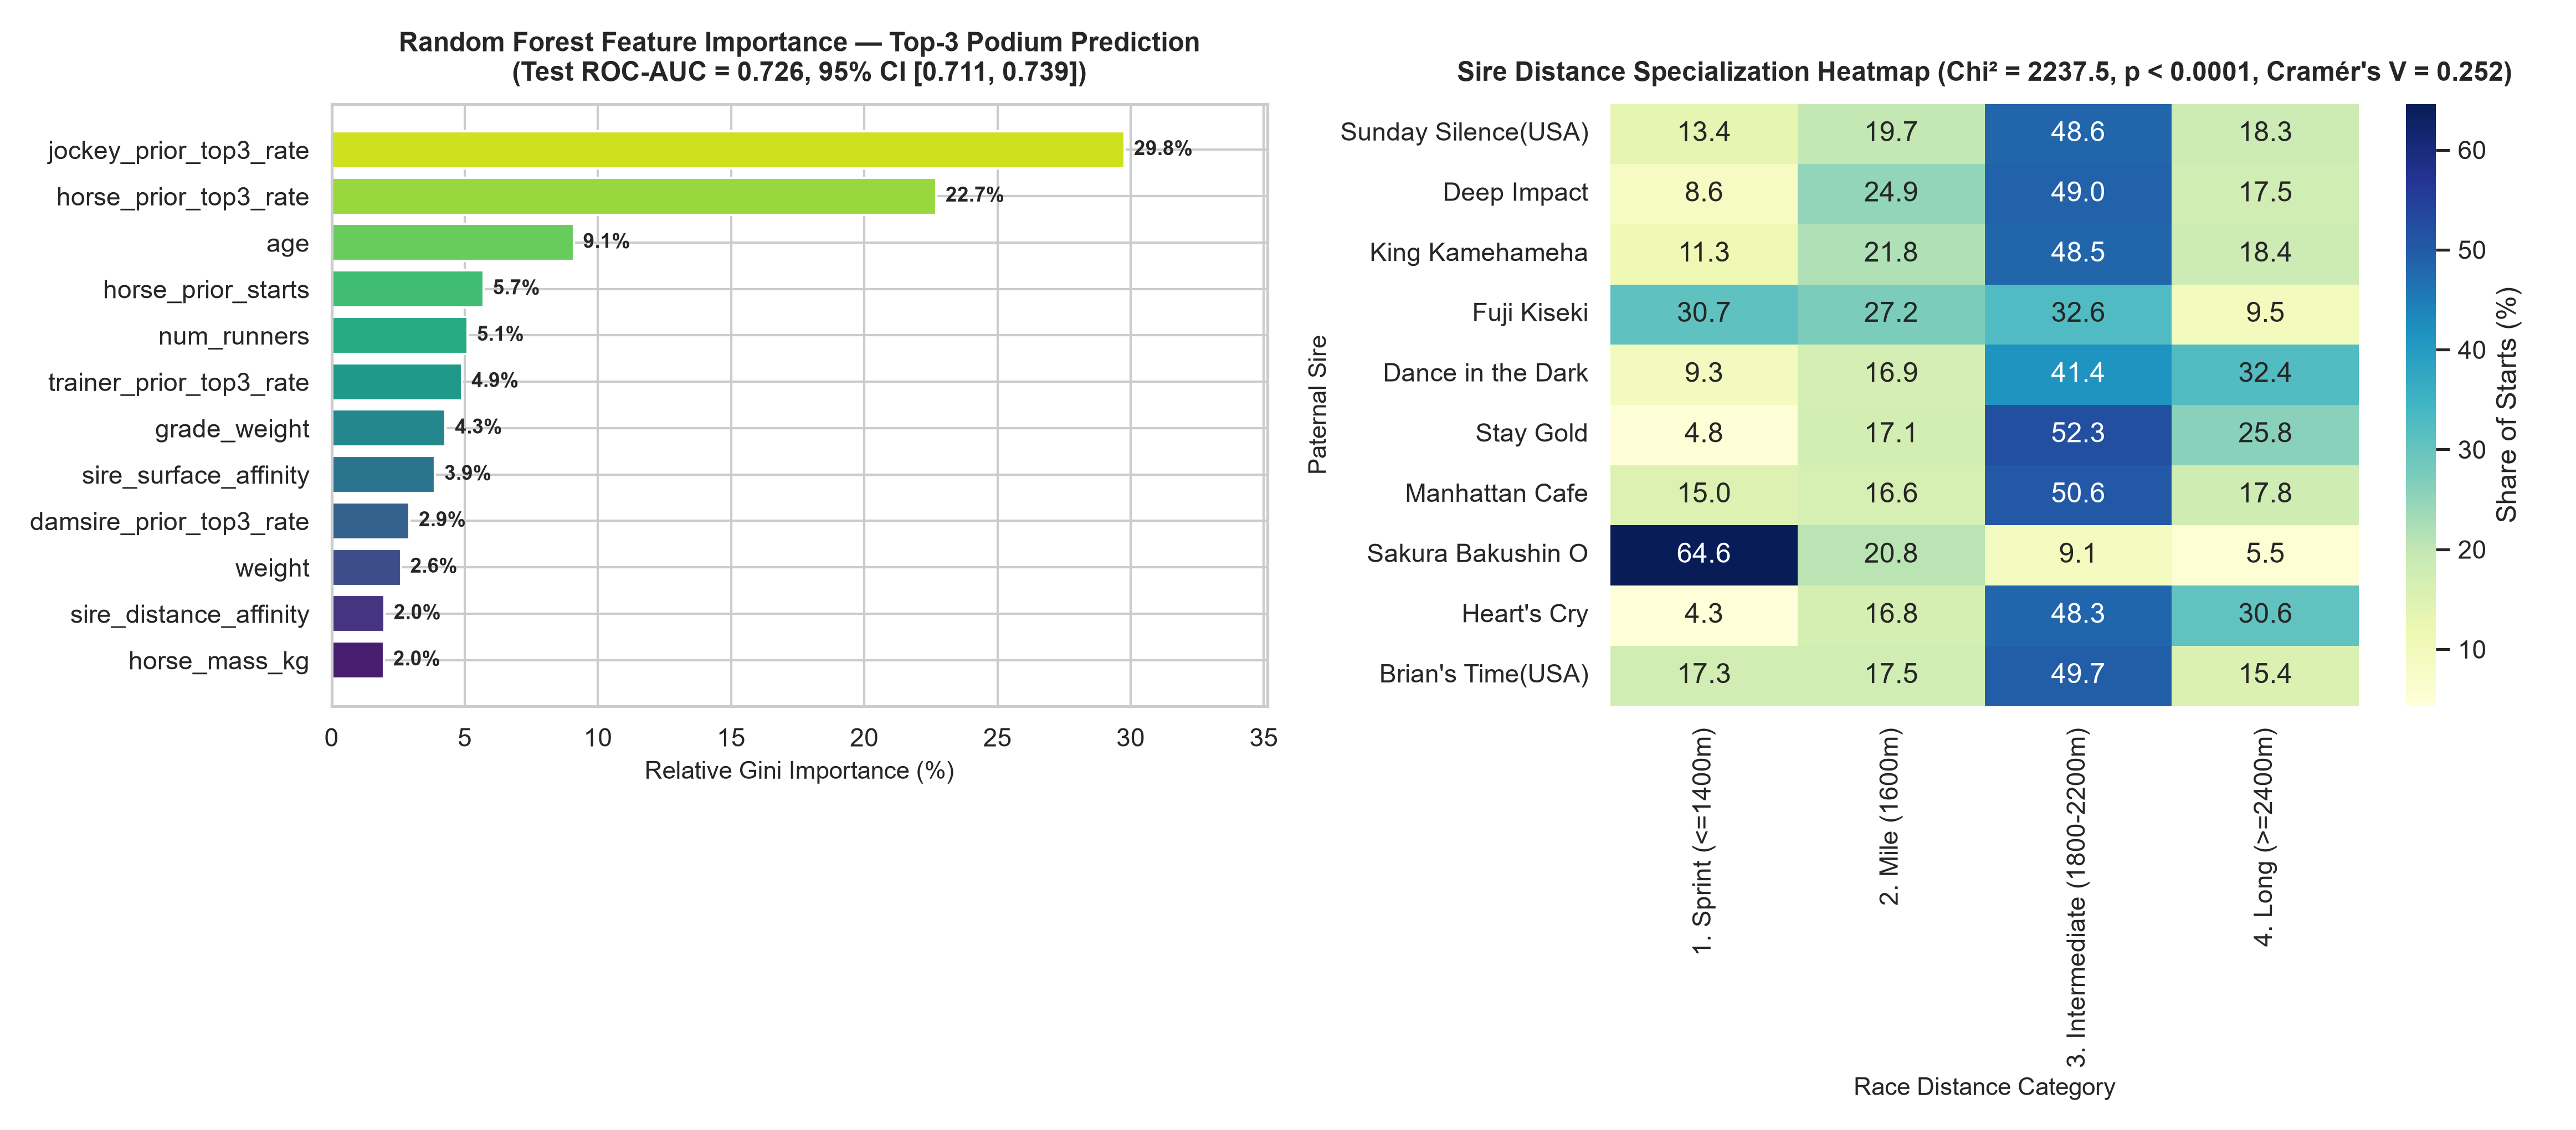
\includegraphics[width=0.94\textwidth]{../assets/ml_random_forest_and_chi2.png}}
\caption{Esquerda: Importância Relativa de Gini (\%) na Random Forest ($\text{ROC-AUC} = 0,7260$). Direita: Mapa de Calor de Especialização Paterna por Distância ($\chi^2 = 2237,5, p < 0,0001$).}
\label{fig:rf_chi2_aeds2}
\end{figure*}

\subsection{Ecossistema Web Interativo: Suíte Apache Superset / ECharts e Gamificação na JRA TCG Card Arena}
Para democratizar a exploração das estruturas em árvores e grafos desenvolvidas neste trabalho sem exigir conhecimento de programação do usuário final, construíram-se duas aplicações web interativas trilíngues (Português, Inglês e Japonês) compiladas pelos módulos \path{src/generate_advanced_viz.py} e \path{src/generate_tcg_cards.py} e hospedadas publicamente via \textit{GitHub Pages} [14]:
\begin{enumerate}
    \item \textbf{Suíte Executiva Interativa Apache Superset 6.1 / Apache ECharts 5.5:} Acessível ao vivo em \url{https://imarthz.github.io/AEDS2_jra_analysis/docs/superset_interactive_dashboard.html} (com edições em inglês em \path{superset_interactive_dashboard_en.html} e japonês em \path{superset_interactive_dashboard_ja.html}). A aplicação integra 6 cartões de indicadores-chave (KPIs) e \textbf{13 gráficos multidimensionais interativos}, incluindo diagrama Sankey aluvial de 4 estágios com realce dinâmico de adjacência, Sunburst hierárquico de 3 anéis com \textit{drill-down} clicável sobre os 10 hipódromos, quadrante de dispersão PageRank com zoom contínuo e Coordenadas Paralelas com filtro deslizante ao vivo (\textit{Live Brush Filter}) sobre os 106 garanhões.
    \item \textbf{Arena Gamificada de Cards e Travessia de Árvores --- JRA \& JBIS TCG Card Arena:} Acessível ao vivo em \url{https://imarthz.github.io/AEDS2_jra_analysis/docs/jra_tcg_arena.html} (suportando seleção direta de idioma via parâmetro \texttt{?lang=pt}, \texttt{?lang=en} ou \texttt{?lang=ja}). A aplicação converte os vértices e métricas topológicas de $G_c$, $G_p$ e $G_{jc}$ em \textbf{520 Cards Colecionáveis distribuídos em 6 decks de ranking} (324 cavalos de elite, 106 garanhões reprodutores, 60 jóqueis e 30 patriarcas fundadores de 5 gerações). Cada card recebe um índice procedural Overall ($\text{OVR } 76\text{--}99$) derivado da combinação ponderada de PageRank, vitórias G1, consistência de pódio e ganhos, classificado em 5 níveis de raridade: \texttt{SSR Mythic}, \texttt{DIAMOND Anomaly} (exclusivo para os ``Diamantes Injustiçados'' com 0 vitórias Graded e altíssimo PageRank, como \textit{Sounds of Earth}), \texttt{SILVER Crown} (0 vitórias G1), \texttt{UR Epic} e \texttt{SR Rare}. Ao clicar em qualquer card, abre-se um \textbf{Dossiê 3D Expandido} contendo o polígono Radar de 6 atributos, o Coeficiente de Wright $F_X$ e uma \textbf{Árvore Genealógica Interativa Clicável}: clicar no nó do Pai (\textit{Sire}), do Avô Materno (\textit{Dam's Sire}), do Jóquei ou dos filhos executa uma travessia instantânea em memória no grafo e abre o card do vértice conectado, além de oferecer um \textbf{Modo Duelo (VS Duel Mode)} para comparação de dois vértices frente a frente.
\end{enumerate}

\section{Conclusão, Reprodutibilidade em Linux e Próximas Etapas}
Este trabalho apresentou uma solução algorítmica completa, fundamentada em estruturas em árvores e teoria dos grafos, para modelar 24 anos de histórico competitivo da \textit{Japan Racing Association} (3.216 corridas, 33.409 participações e 8.209 cavalos) integrados às árvores genealógicas ascendentes de 5 gerações do \textit{Japan Bloodhorse Information System} (504.074 nós ancestrais).

Em síntese, as principais contribuições científicas e computacionais alcançadas foram:
\begin{enumerate}
    \item \textbf{Resolução da Bijeção Topológica $\text{DFS}\to\text{BFS}$ e Contração no DAG $G_p$:} A formulação da permutação exata $\Phi$ entre a ordem de pré-ordem DFS e a ordem de nível BFS corrigiu 504.074 ligações pai-filho e permitiu colapsar as árvores individuais em um DAG unificado ($|V_p| = 35.149, |E_p| = 63.007$), sobre o qual travessias BFS/DFS, consultas de Menor Ancestral Comum (LCA) e o Coeficiente de Endogamia de Wright ($F_X$) executam na casa de dezenas de microssegundos por animal, comprovando \textit{Northern Dancer (CAN)} como o maior ancestral comum duplicado ($4.206$ cavalos e $1.211$ vitórias Graded) e \textit{Almahmoud (USA)} ($0,400$ vitórias Graded/animal) seguida por \textit{Halo (USA)} ($0,373$ vitórias/animal) como os ancestrais de maior eficiência competitiva endogâmica no Top 10.
    \item \textbf{Descoberta de Talentos Ocultos via PageRank Esportivo em $O(V + E)$:} A modelagem do fluxo de prestígio em $G_c$ ($|V_c| = 8.135, |E_c| = 195.271$) superou a cegueira da contagem simples de vitórias ao identificar os ``Diamantes Injustiçados'' (liderados por \textit{Sounds of Earth}, \#32 geral entre 8.135 cavalos com zero vitórias Graded) e confirmou uma Componente Gigante Conexa abrangendo $98,66\%$ da população histórica.
    \item \textbf{Sinergia entre Topologia Genealógica, Fator Humano e Visualização Interativa:} Provou-se estatisticamente que a linhagem paterna no DAG define o nicho físico de superfície e distância ($\chi^2 = 2237,47, p < 10^{-300}$, 4 arquétipos no K-Means++ PCA com $63,4\%$ de variância e dimorfismo biométrico de $+18\text{ kg}$ na areia), enquanto na hora da corrida o histórico prévio do jóquei ($29,77\%$ de importância de Gini) e do cavalo ($22,70\%$) governam a predição de pódio na \textit{Random Forest Out-of-Time} ($\text{ROC-AUC} = 0,7260$ com \textit{Zero Data Leakage}), resultados estes traduzidos visualmente nos grafos vetoriais Gephi, na suíte \textit{Apache Superset / ECharts} e na arena gamificada \textit{JRA TCG Card Arena}.
\end{enumerate}

\subsection{Desafios, Limitações e Sugestões para Pesquisas Futuras}
Durante o desenvolvimento, os principais desafios e limitações enfrentados compreenderam: (i) a heterogeneidade estrutural das páginas históricas da JRA (2002--2025), que exigiu algoritmos de realinhamento vetorial para corrigir 25.014 linhas deslocadas; (ii) a presença de 15 campeões internacionais homônimos nos registros ascendentes de 5 gerações, solucionada por regras de desambiguação temporal; e (iii) a ausência, nas tabelas públicas resumidas da JRA anteriores a 2010, das parciais cinemáticas individuais de cada seção de $200\text{m}$ (\textit{sectional furlong times}) e da biometria das matrizes mães (\textit{Dams}) que não competiram em provas graduadas.

Como direções promissoras para pesquisas futuras, propõem-se:
\begin{itemize}
    \item \textbf{Redes Neurais em Grafos (\textit{Graph Neural Networks} --- GNNs / GraphSAGE):} Acoplar diretamente a matriz de adjacência do DAG de 5 gerações $G_p$ e do grafo bipartido $G_{jc}$ a camadas de passagem de mensagens (\textit{Message Passing Neural Networks}) para aprender \textit{embeddings} genealógicos profundos fim a fim;
    \item \textbf{PageRank Temporal com Decaimento Exponencial (\textit{Time-Decaying PageRank}):} Introduzir um kernel de amortecimento temporal $e^{-\lambda \Delta t}$ nas arestas de $G_c$ para capturar flutuações sazonais de forma atlética entre os 3 e os 6 anos de idade;
    \item \textbf{Algoritmos de Fluxo Máximo e Emparelhamento Bipartido Ótimo:} Aplicar o algoritmo de Hopcroft-Karp / Kuhn-Munkres (Algoritmo Húngaro) sobre o grafo bipartido ponderado $G_{jc}$ para recomendar a alocação ótima de jóqueis disponíveis para um grid de largada de Grau 1.
\end{itemize}

\subsection{Instruções Objetivas de Execução e Validação no Linux (Ubuntu 24.04)}
Para assegurar a reprodutibilidade científica integral, todo o código-fonte (\url{https://github.com/ImArthz/AEDS2_jra_analysis}) e a base de dados arquivada no Zenodo (\url{https://doi.org/10.5281/zenodo.23681383} / \url{https://zenodo.org/records/24498336}) [14] são 100\% compatíveis com execução via terminal no \textbf{Linux (Ubuntu 24.04 LTS)} sem necessidade de configurações excepcionais (o banco SQLite higienizado \path{data/sqlite/jra_graded_en.db}, os CSVs bilíngues e o cache de tradução \path{data/gemini_cache.json} já acompanham o pacote para execução offline imediata):
\begin{footnotesize}
\begin{verbatim}
git clone https://github.com/ImArthz/AEDS2_jra_analysis.git
cd AEDS2_jra_analysis
python3 -m venv .venv && source .venv/bin/activate
pip install -r requirements.txt
python3 src/validate_data.py
python3 src/graph_analysis.py
python3 src/ml_analysis.py
python3 src/generate_advanced_viz.py
python3 src/generate_tcg_cards.py
\end{verbatim}
\end{footnotesize}

\begin{thebibliography}{14}
\bibitem{cormen2022} T. H. Cormen, C. E. Leiserson, R. L. Rivest, and C. Stein, \textit{Introduction to Algorithms}, 4th ed. Cambridge, MA, USA: MIT Press, 2022.
\bibitem{tarjan1972} R. Tarjan, ``Depth-first search and linear graph algorithms,'' \textit{SIAM Journal on Computing}, vol. 1, no. 2, pp. 146--160, 1972.
\bibitem{wright1922} S. Wright, ``Coefficients of inbreeding and relationship,'' \textit{The American Naturalist}, vol. 56, no. 645, pp. 330--338, 1922.
\bibitem{bender2005} M. A. Bender, M. Farach-Colton, G. Pemmasani, S. Skiena, and P. Sumazin, ``Lowest common ancestors in trees and directed acyclic graphs,'' \textit{Journal of Algorithms}, vol. 57, no. 2, pp. 75--94, 2005.
\bibitem{pagerank1999} L. Page, S. Brin, R. Motwani, and T. Winograd, ``The PageRank citation ranking: Bringing order to the web,'' Stanford InfoLab, Stanford University, Stanford, CA, USA, Tech. Rep. 1999-66, 1999.
\bibitem{brin1998} S. Brin and L. Page, ``The anatomy of a large-scale hypertextual Web search engine,'' \textit{Computer Networks and ISDN Systems}, vol. 30, no. 1--7, pp. 107--117, 1998.
\bibitem{gleich2015} D. F. Gleich, ``PageRank beyond the Web,'' \textit{SIAM Review}, vol. 57, no. 3, pp. 321--363, 2015.
\bibitem{dijkstra1959} E. W. Dijkstra, ``A note on two problems in connexion with graphs,'' \textit{Numerische Mathematik}, vol. 1, no. 1, pp. 269--271, 1959.
\bibitem{newman2010} M. E. J. Newman, \textit{Networks: An Introduction}. Oxford, UK: Oxford University Press, 2010.
\bibitem{gephi2009} M. Bastian, S. Heymann, and M. Jacomy, ``Gephi: An open source software for exploring and manipulating networks,'' in \textit{Proc. Int. AAAI Conf. Weblogs and Social Media (ICWSM)}, San Jose, CA, USA, 2009, pp. 361--362.
\bibitem{jacomy2014} M. Jacomy, T. Venturini, S. Heymann, and M. Bastian, ``ForceAtlas2, a continuous graph layout algorithm for handy network visualization designed for the Gephi software,'' \textit{PLOS ONE}, vol. 9, no. 6, p. e98679, 2014.
\bibitem{arthur2007} D. Arthur and S. Vassilvitskii, ``k-means++: The advantages of careful seeding,'' in \textit{Proc. 18th Annu. ACM-SIAM Symp. Discrete Algorithms (SODA)}, New Orleans, LA, USA, 2007, pp. 1027--1035.
\bibitem{breiman2001} L. Breiman, ``Random forests,'' \textit{Machine Learning}, vol. 45, no. 1, pp. 5--32, 2001.
\bibitem{mendonca_zenodo_aeds2} A. D. O. Mendonça and M. P. da Silva, ``JRA Graded Races (2002--2025) \& JBIS 5-Generation Pedigree Dataset (Bilingual JA/EN + Graph Networks, Apache Superset Suite \& TCG Card Arena),'' \textit{Zenodo (CERN/OpenAIRE)}, v1.0.25, 2026, doi: 10.5281/zenodo.23681383. [Online]. Available: \url{https://zenodo.org/records/24498336} e Repositório de Código-Fonte (GitHub): \url{https://github.com/ImArthz/AEDS2_jra_analysis}
\end{thebibliography}

\end{document}
